\documentclass{kththesis}

\usepackage{csquotes} % Recommended by biblatex
\usepackage[style=numeric,sorting=none,backend=biber]{biblatex}
\addbibresource{references.bib} % The file containing our references, in BibTeX format

\usepackage{amsmath}
\usepackage{amssymb}
\usepackage{graphicx}
\usepackage{hyperref}
\usepackage{caption}
\usepackage{subcaption}

\title{A deep reinforcement learning approach to the problem of golf using an agent limited by human data}
\author{Fredrik Omstedt}
\email{omstedt@kth.se}
\supervisor{Arvind Kumar}
\examiner{Erik Fransén}
\programme{Master in Computer Science}
\school{School of Electrical Engineering and Computer Science}
\date{\today}

% Uncomment the next line to include cover generated at https://intra.kth.se/kth-cover?l=en
\kthcover{kth-cover.pdf}

\begin{document}

% Frontmatter includes the titlepage, abstracts and table-of-contents
\frontmatter

\titlepage

\begin{abstract}
In the sport of golf, the use of statistics has become prominent as a way of understanding and improving golfers' golf swings. Even though swing data is easily accessible thanks to a variety of technical tools, it is not always clear how to use this data, especially for amateur golfers. This thesis investigates the feasibility of using reinforcement learning in conjunction with a golfer's data to play golf, something that could provide insight on how the golfer can improve. Specifically, a Dueling Double Deep Q Network agent and a Multi Pass Deep Q Network agent were trained and evaluated on playing golf from pixel data on two simulated golf courses, using only shot data provided by a real golfer to hit shots. These two reinforcement learning agents were then compared with the golfer on how well they played, in regards to the number of shots hit and distances remaining to the golf holes when the holes were finished. The majority of the results showed no significant difference between either agent and the golfer on both golf courses tested, indicating that the agents could play on a similar level to the golfer. The complexity of the problem caused the agents to have a good knowledge of states that occurred often but poor knowledge otherwise, which is one likely reason why the agents played similarly to but not better than the golfer. Other reasons include lack of training time, as well as potentially non-representative data retrieved from the golfer. It is concluded that there is potential in using reinforcement learning for the problem of golf and possibly in similar problems as well. Moreover, further research could improve the agents such that more valuable insights regarding golfers' data can be found.
\end{abstract}

\begin{otherlanguage}{swedish}
\begin{abstract}
Inom sporten golf har användandet av statistik blivit ett vanligt sätt att förstå och förbättra golfares golfsvingar. Trots det faktum att svingdata är tillgängligt, tack vare en mängd tekniska verktyg, är det inte självklart hur datan kan användas, speciellt för amatörgolfare. Detta examensarbete undersöker huruvida användandet av förstärkande inlärning tillsammans med en golfares data är en möjlighet för att spela golf, något som skulle kunna bidra med insikter om hur golfaren kan utvecklas. Mer specifikt har en Dueling Double Deep Q Network-agent och en Multi Pass Deep Q Network-agent tränats och evaluerats på att spela golf från pixeldata från två simulerade golfbanor genom att endast använda slagdata från en riktig golfare. Dessa två agenter har sedan jämförts med golfaren på hur väl de spelade i förhållande till mängden slag och avstånden till golfhålen när hålen avslutats. Majoriteten av resultaten visade ingen signifikant skillnad mellan någon av agenterna och golfaren på båda golfbanorna, vilket indikerar att agenterna spelade på en liknande nivå som golfaren. Komplexiteten hos problemet gjorde att agenterna hade bra kunskap om tillstånd som förekom ofta men dålig kunskap annars. Detta är en trolig orsak till att agenterna kunde spela på en liknande nivå som men inte bättre än golfaren. Andra anledningar kan vara för lite träningstid och potentiellt ickerepresentativ data från golfaren. Sammanfattningsvis kan slutsatsen dras att användandet av förstärkande inlärning för problemet golf, och möjligtvis även liknande problem, har potential. Dessutom skulle agenterna kunna förbättras givet fler eller mer djupgående undersökningar, så att mer värdefulla insikter om golfares data kan upptäckas.
\end{abstract}
\end{otherlanguage}

\newenvironment{acknowledgements} {\renewcommand\abstractname{Acknowledgements}\begin{abstract}} {\end{abstract}}

\begin{acknowledgements}
To my family, for their continuous support that led me to this moment. To my supervisors, for their insight and helpful comments. To my friends, for making the journey fun.
\end{acknowledgements}

\tableofcontents

% Mainmatter is where the actual contents of the thesis goes
\mainmatter

%HOW TO CITE:
%\parencite{ref} = [1]
%\parencite{ref2} = Einstein [2]

\chapter{Introduction}
\label{chapter:introduction}
Golf is a sport in which a player attempts to hit a ball into a hole using clubs, from a given starting position, with as few strokes as possible. It is a widely popular sport, with golf courses and active players all around the world. Due to the technical skills required to perform a good golf swing, many teachers, professionals as well as amateur golfers have started using statistics to try and understand and improve their golf swings. This need of data has caused a surge in technical tools such as launch monitors that analyze the golf swing as a player hits a ball, and tracking software that looks at the golf shots while in the air. 

Even though swing and shot data is more easily accessible than before it is not always inherently clear how to use this data. Professional golfers as well as teachers usually know enough about golf swings to understand how their shot and swing data affects their results, and how to improve their game using it, but amateurs seldom have the time nor knowledge required to efficiently do so. This can be remedied by lessons from teachers, but lessons can become expensive since consistent updates are usually required for noticeable improvements. 

In the past decade, there have been plenty of research done in the field of artificial intelligence for games. Specifically, the work done by Google DeepMind in \parencite{mnih2015human} showcased methods capable of exceeding human levels of play in several Atari games. This research caused much more work to be done in the field, and now there are artificial agents capable of beating 99.8\% of players in the immensely complex game StarCraft II \parencite{vinyals2019grandmaster}. 

The methods used in the above mentioned examples are all based on reinforcement learning. At its core, reinforcement learning is a method in which a so called agent learns how to perform a task in a given environment by observing the environment, performing actions, and analyzing the effects of those actions on the environment. By being punished or rewarded, the agent can learn which actions to take given a specific environment. Traditionally, these types of algorithms have worked for relatively simple environments, but the Dueling Q Network algorithm in \parencite{mnih2015human} showed that this is also possible in complex environments through the use of deep neural networks. This deep reinforcement learning has now been applied to several different types of problems, such as the Deep Deterministic Policy Gradient algorithm presented in \parencite{lillicrap2015continuous} for continuous action spaces, and is a baseline for the state of the art in this field.

As can be seen from above, reinforcement learning is capable of creating well performing agents for various games. It is therefore interesting to investigate if this approach could be utilized to create an agent for the game of golf, since golf is easily adaptable to a reinforcement learning problem in that the agent will hit golf shots (the actions) on a golf course (the environment) such that it minimizes the number of strokes performed (the penalty). Furthermore, it is interesting to see if an artificial agent could learn how to utilize data from golf shots when playing. If that is the case, then real golfers' data could be used with the agent, resulting in the agent being able to show the golfers how their data can improve their game. If successful, this could then be generalized to other similar areas, such as basketball players trying to throw balls into hoops, or robots trying to learn tasks utilizing human data.

\section{Research Question}
Given the description above, the research question investigated in this thesis is the following:
\begin{quote}
    How well does a reinforcement learning agent, limited by shot data from a golfer, play golf compared to the golfer whose data it uses?
\end{quote}
This research question entails implementing a reinforcement learning agent capable of playing golf. Furthermore, this agent must be limited by shot data from a golfer. That is, the actions of the agent will be dependent on the shots from a human. Finally, the question requires a comparison between the golfer and the agent in regards to playing golf. 

\section{Purpose}
This thesis investigates the feasibility of training reinforcement learning agents to play golf. This is, as mentioned above, useful for several reasons. First of all, an agent capable of playing better than the golfer whose data it is limited by knows more about the golfer's shot data than the golfer. This allows the agent to be used as a learning tool to help golfers improve their game. This can not only help golfers minimize the costs from taking lessons, but might also be useful for trainers when teaching.

From a broader perspective, the purpose of this thesis is also to investigate the usability of reinforcement learning in general. Papers such as \parencite{mnih2015human} showcase that it is possible to create agents capable of performing tasks on a high level, but these tasks are still specific to certain environments. The results in this thesis may generalize these results by not only showcasing how well an agent can play golf, but also looking into how reinforcement learning can be combined with human data. This latter reason can in turn provide insight into other similar problems, where reinforcement learning has not yet been attempted. 

\section{Scope}
While the end goal of the work in this paper is to have agents that can act as learning tools for golfers, this goal is outside of the scope of this thesis. The first step towards this goal is to look into the feasibility of using reinforcement learning agents for the problem of golf, which is what is investigated in this paper.

The term reinforcement learning is broad. For the scope of this thesis, two types of reinforcement learning algorithms are implemented and tested, the Dueling Double Deep Q Network algorithm presented in \parencite{wang2015dueling} and the Multi Pass Deep Q Network algorithm presented in \parencite{bester2019mpdqn}. These algorithms were chosen because they fit well with the problem of golf. This will be explained further in \autoref{chapter:background} and \autoref{chapter:methods}.

Just like with reinforcement learning, the term golf is also broad. For the scope of this thesis, the agents will be trained, evaluated and compared with a golfer on two golf courses: Pebble Beach and Ullna GC. These courses were chosen because of them being the courses that data was gathered from by a golfer. 

\section{Disposition}
In \autoref{chapter:background}, information necessary for the understanding of this paper is presented. This chapter includes information about golf, reinforcement learning, as well as neural networks. It also provides some insight into work related to this paper.

In \autoref{chapter:methods}, the methods used to answer the research question are showcased. The tools needed to train the reinforcement learning agent are presented, and how the agents were implemented, trained and evaluated is described. Moreover, the data gathering process from a golfer is touched upon.

In \autoref{chapter:results}, the results from the data gathering process as well as the evaluation of the reinforcement learning agents implemented is presented. The agents are compared to the golfer and statistical tests are performed to determine the significance of the results. 

In \autoref{chapter:discussion}, the results are analyzed to draw conclusions regarding the research question. Moreover, limitations on this thesis are presented and discussed, and future research is touched upon.

Finally, in \autoref{chapter:conclusions}, the conclusions drawn from \autoref{chapter:discussion} are summarized.

\chapter{Background}
\label{chapter:background}
In this chapter, the background information necessary for the understanding of this thesis is described. Moreover, work related to this paper is presented.

\section{Golf}
\label{sec:golf}
Golf is a sport in which players use clubs to, starting from a predetermined position, hit balls into holes on a course using as few strokes as possible. The golf course is, unlike in many other sports, not a standardized playing area. Instead, one goal of the game is to be able to adapt to the various surroundings on a course. More specifically, a golf course usually consists of nine or 18 holes, each of different nature. Every hole on the course has a fixed distance, determined by the starting position, commonly known as the tee box, and the actual hole, always located on the putting green. Both the tee box and and the green consists of short cut grass areas, with the green usually being especially well maintained.

Aside from the existence of one or several tee boxes and a green, the holes on a course can look very different from one another. However, they all contain a subset of the same types of terrain:
\begin{itemize}
    \item The fairway - a short cut grass area positioned in the intended playing area of the hole. 
    \item The rough - a long cut grass area positioned around the fairway.
    \item Bunkers - sand traps positioned at various locations on the hole. These usually have a edges making them hard to escape.
    \item Water hazards - areas of water from which it often is impossible to hit shots.
    \item Native areas - areas of vegetation such as woods or swamps. These usually enclose the hole.
    \item Pathways - man made paths used for walking or driving golf carts on.
    \item Out of bounds - areas outside the course. It is not allowed to play from these areas.
\end{itemize}
An example of a golf hole can be found in \autoref{fig:golfhole}.\footnote{\url{https://en.wikipedia.org/wiki/File:Golf_field.svg} under the Creative Commons license (Accessed 2020-04-15).}

\begin{figure}
    \centering
    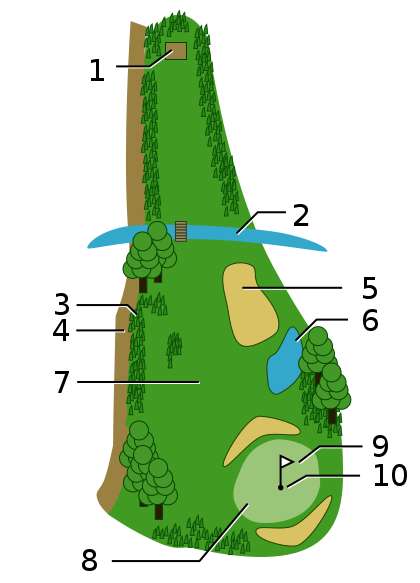
\includegraphics[width=0.4\textwidth]{golffield.png}
    \caption{An example of a golf hole as seen from above. The tee box is labelled with a 1 and the green with an 8. The hole contains a fairway (7), rough (3), native areas, water hazards (2, 6), bunkers (5), as well as an out of bounds area (4).}
    \label{fig:golfhole}
\end{figure}

The difficulty of each hole is determined using an index named par. The par of a hole tells a golfer how many shots generally are expected to be hit by a professional golfer before they reach the hole. This value is usually directly correlated to the distance of the hole. In most cases, the pars of the holes on a course range from three to five, but other values exist as well. The par also determines the maximum number of shots allowed to be hit on a hole, with this number being the par of the hole plus five. This limit is not mandatory, and most professional competitions require the ball to be holed no matter the number of shots hit.

A round of golf is played by completing a number of holes, usually nine or 18, in a given order. This order is usually determined by the layout of the golf course. Each hole starts by the golfer hitting a shot from the tee box. The golfer then goes to the place where the ball stopped and continues hitting towards the hole. This is repeated until the ball is resting in the hole.

Golfers utilize different clubs to hit their shots. Each club looks different from the others, such as in the length of the shaft, the loft of the club face, or the shape of the club head. These clubs can broadly be divided into four categories; woods, irons, wedges and the putter. Woods have large club heads and long shafts, making them able to generate a high speed. This causes the shots hit with woods to travel longer than other clubs. Woods generally have a smaller degree of loft. Irons have flat club heads and are mainly used for medium length shots. Wedges also have flat club heads but with a greater amount of loft, at least 40 degrees. They are most often used for short shots outside of the green. The putter varies in club head shape, but generally has no or a small degree of loft. It is used for rolling shots, mainly on the putting green. To separate different clubs within the different groups, numbers are often used. These numbers are dependent on the loft of the club, with a lower number indicating a lower loft. For instance, a 4 Iron has a lower loft than a 7 Iron.

A golfer is allowed to have 14 clubs with them during a round of golf. Generally, a mix of all types of clubs is required to perform as wide of an array of shots as possible. In most cases, a golfer can, with some accuracy, map a full swing of a club to a certain distance, and therefore utilizes this knowledge in order to play the game. For shorter shots, however, more feel is usually required than for full swing shots.

In most cases, the ball is played as it lies. That is, wherever the ball stopped, the player has to continue hitting from. In some cases, however, this may not be possible. For instance, a wayward shot might be positioned in an out of bounds area or at the bottom of a lake. In such cases, the player may elect (or is forced) to drop the same or, in some cases, a new ball from a different position than the ball's current position, and play from there instead. In most cases, this results in the player incurring a penalty of a set amount of strokes. The new position to drop the ball on is determined based on the reason for dropping the ball. 

In order for golfers of different skill levels to play against each other, a system known as the handicap system has been developed. This system gives each player a handicap, an index that describes how good a golfer is. This index can be used to determine how well a golfer is expected to play at a given course. Each course is given a slope rating, and this rating together with a handicap can determine the expected number of shots to be hit by a golfer in a round. As such, golfers of different skill levels can compete against one another by comparing their deviation from their expected number of shots, rather than comparing their number of shots directly.

Due to the nature of the game, golf is easily adaptable to a digital setting. It contains well defined rules, is played on specified areas (the golf holes) and allows for a specific set of actions (hitting shots with golf clubs). These components can be described digitally, allowing golf to be played in a virtual environment. As such, this allows for artificial agents to be trained for playing golf, since they can access the game digitally. The agents have, regardless of using deterministic rules or learning methods, access to the data related to the game, which results in the possibilities of helping golfers improve using artificial intelligence.

\section{Reinforcement Learning}
\label{sec:reinforcementlearning}
Humans learn through interacting with their environment. For instance, a child does not have a teacher teaching it how to move its joints to walk, but rather observes its environment (such as adults moving around it) and tries actions to propel itself forward. It learns how its actions affect its environment and how much they contribute to the success of the process. Eventually, the child learns to walk successfully. 

Reinforcement learning is a learning process imitating the above mentioned way humans learn. More specifically, it deals with the problem of mapping actions to observations such that a reward value is maximized. In the case of the child learning to walk, this directly corresponds to the child mapping joint movements to its position and pose in a room such that it stays upright while moving forwards as well as possible. With reinforcement learning, the learner does not know which actions to take, but must instead figure out which actions result in the highest reward simply by trying them. In some cases, the reward may not appear immediately, but follow from subsequent actions taken. Reinforcement learning therefore also takes the concept of delayed rewards into account. \parencite{sutton1998introduction}

A reinforcement learning system contains several components that make it possible to learn how to achieve a goal: the \textit{environment}, the \textit{state}, the \textit{actions}, the \textit{reward}, the \textit{policy}, the \textit{agent} and the \textit{action-value function}.

The \textit{environment} describes the world encapsulated by the problem the reinforcement learning system tries to solve. It contains information about how close to the goal the system is, as well as which actions are possible to take. For instance, an environment could be a maze containing a robot, with the goal being the robot exiting the maze.

The \textit{state} is a snapshot of the environment. It details information about a specific part of the environment. For instance, a state of an environment could be the current position of a robot in a maze.

The \textit{actions} determine the possible things to do in an environment. The actions modify the current state of the environment into a new one. For instance, the actions of an environment could be the movement of a robot in a maze. 

The actions are contained in the action space. The dimensionality of the action space determines the number of actions to be taken. The actions can be either discrete, continuous, or both. A discrete action consists of choosing between one of several options, such as moving a robot either up, right, down or left in a maze. A continuous action consists of choosing real values, such as how many meters to move a robot in a given direction in a maze.

An action space is named depending on its actions. Discrete action spaces contain only discrete actions, continuous action spaces contain only continuous actions, and hybrid action spaces contain both types of actions. As will be shown in the following subsections of \autoref{sec:reinforcementlearning}, some algorithms work better for different types of action spaces.

The \textit{reward} indicates how good a certain state in the environment is. The higher the reward is, the better the state is to be in. In some cases, it makes more sense to use a \textit{punishment}, where a high number showcases a bad state. For instance, a punishment could be the distance between a robot in a maze and the maze's exit. 

The \textit{agent} is the learner in the reinforcement learning system. It receives states and rewards as input, and outputs the actions to take.

The \textit{policy} is a description of how the agent takes actions given certain states and rewards. The policy is at the center of the reinforcement learning system, since the system tries to learn how to best take actions in an environment. \parencite{sutton1998introduction}

Rewards only indicate the immediate result of an action. The \textit{action-value function} is therefore used to specify long term rewards. The value of a state can be seen as the reward over time, starting from that state. This action-value function is defined as the Q-function, described in \autoref{eq:qfunction}, where $\pi$ is the policy used, $s$ the current state, $a$ the action chosen, $R_t$ the current reward and $R_{t+1}$ etc. the future rewards from the subsequent states. $\gamma$ is a discount factor used to determine the importance of future rewards compared to immediate ones. The optimal value is then determined by the optimal action-value function, defined in \autoref{eq:qoptimal}. By choosing the highest valued action for each state, the optimal policy is easily found. \parencite{van2016deep}

\begin{equation}
\label{eq:qfunction}
Q_\pi(s, a) = \mathbb{E}[R_t + \gamma R_{t+1} + \gamma^2R_{t+2} + ... | S_t = s, A_t = a, \pi]
\end{equation}

\begin{equation}
\label{eq:qoptimal}
Q_*(s, a) = max_\pi Q_\pi(s, a)
\end{equation}

Just like there is an action-value function, there is also a state-value function, defined in \autoref{eq:statevalue}. In this equation, $a\sim\pi(s)$ represents the action $a$ as chosen by the policy $\pi$ in state $s$.
\begin{equation}
\label{eq:statevalue}
V_\pi(s) = \mathbb{E}_{a\sim\pi(s)}[Q_\pi(s,a)]
\end{equation}
Whereas the action-value function indicates how good an action is in a state, the state-value function indicates how good a state is in general. \parencite{wang2015dueling}

A relevant function to the above defined functions is the advantage function, defined in \autoref{eq:advantage}. This equation subtracts the state-value from the action-value to showcase the relative performance of an action in a state. \parencite{wang2015dueling}

\begin{equation}
\label{eq:advantage}
A_\pi(s,a) = Q_\pi(s,a) - V_\pi(s)
\end{equation}

For an illustration of how the above mentioned components interact with each other, see \autoref{fig:reinforcementlearning}\footnote{\url{https://commons.wikimedia.org/wiki/File:Markov_diagram_v2.svg} under the Creative Commons license (Accessed 2020-04-15)}.

\begin{figure}
\centering
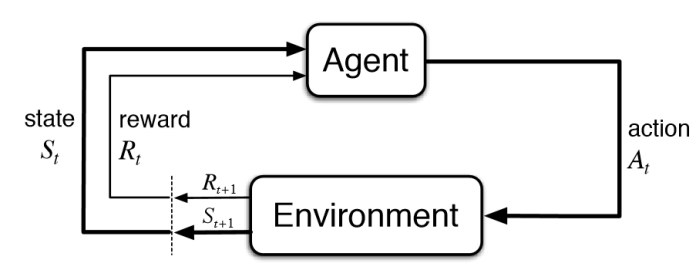
\includegraphics[width=0.75\textwidth]{reinforcement-learning.jpg}
\caption{A representation of how reinforcement learning works. The environment sends a state and reward to the agent, which utilizes this information together with its policy to choose an action input to the environment, resulting in a new state and a corresponding reward.}
\label{fig:reinforcementlearning}
\end{figure}

\subsection{Exploration versus exploitation}
\label{subsec:explorevsexploit}
One dilemma in the reinforcement learning field is the exploration and exploitation trade-off. This trade-off relates to how an agent maximizes the reward. By performing actions and observing the states, the agent learns which actions yield a high reward. To maximize the reward, the agent has to take these valuable actions it has previously tried. However, it cannot discover these useful actions without trying actions it has never taken before. The agent must exploit what it already knows to get rewarded, but at the same time explore new actions to increase its knowledge. These approaches cannot be taken simultaneously. Due to this, and due to the fact that actions usually must be taken several times to be reliably estimated by the value function, it is hard to determine the trade-off between exploration and exploitation.

For discrete action spaces, one possible solution is the use of the $\epsilon$-greedy policy. With a probability $\epsilon$ a random action is uniformly sampled from the action space, and with a probability $1 - \epsilon$, the best action is chosen. The value for $\epsilon$ usually starts at $1$ to favour exploration at the start of the learning process. It then decreases over time and settles at a low value in order to still allow for some exploration once the agent has learned about the available actions and how they affect the environment. \parencite{sutton1998introduction}

For continuous action spaces the $\epsilon$-greedy policy is infeasible due to the infinite number of choices available in choosing real numbers. Instead, a useful way of introducing exploration is to add random noise to the numbers chosen. This causes the agent to end up in new states, allowing it to learn more about the environment and the actions. The scale of the noise can be reduced during training once the agent starts learning. \parencite{lillicrap2015continuous}

\subsection{Q-learning}
\label{subsec:qlearning}
Q-learning, described in \parencite{watkins1992q}, is a reinforcement learning algorithm. The algorithm works by approximating the optimal action-value function, defined in \autoref{eq:qoptimal}, using a table for storing the so called Q-values of the function. These values are iteratively updated using dynamic programming according to \autoref{eq:qupdate}, where $\alpha$ is a learning rate used to smoothen the learning. 
\begin{equation}
\label{eq:qupdate}
Q(s_t, a_t) \leftarrow Q(s_t, a_t) + \alpha \cdot (R_t + \gamma \cdot max_a Q(s_{t+1}, a) - Q(s_t, a_t))
\end{equation}
As can be seen in the equation, the updated Q-value for a state and action depends on the best possible Q-value in the next state, which is an approximation of all future rewards. Given enough iterations and a good exploration policy, the Q-values converge towards their correct values \parencite{watkins1992q}.

\subsection{Deep Q-learning}
\label{subsec:deepqlearning}
One problem with the Q-learning algorithm is that a table for storing Q-values is infeasible for environments with large state spaces. One example of such an environment is when an agent receives colored images as input, i.e. it observes a rendered representation of a problem. An image usually consists of tens of thousands of pixels. Environments utilizing images can have many different image states, making it impossible to store all this information in a table.

Artificial neural networks (described in detail in \autoref{sec:neuralnetworks}) can be used to approximate models with high dimensional inputs such as images. As such, they seem like good candidates to replace tables for mapping states to actions. That is, the state of the environment can be used as input to a neural network, and the Q-values for each action can be approximated as output from the network. However, reinforcement learning algorithms have been known to diverge when used with non-linear classifiers \parencite{tsitsiklis1997analysis}. This is due to subsequent states being related to each other, major policy changes caused by small updates of the Q function, as well as the correlations between action values and their so called target values $Y$, defined in \autoref{eq:qtarget}.

\begin{equation}
\label{eq:qtarget}
Y_t = R_t + \gamma \cdot max_a Q(s_{t+1}, a)
\end{equation}

The deep Q-network algorithm (DQN) presented in \parencite{mnih2015human} utilizes a deep neural network to approximate the action-value function. It solves the problems mentioned above by introducing two features to the network: the use of something known as experience replay, and by updating the Q-values with target values only updated periodically. 

Experience replay, described in \parencite{lin1992self}, is a process in which the agent stores experiences, defined as $e_t = (s_t, a_t, R_t, s_{t+1})$, every iteration in a buffer. This buffer stores the $m$ most recent experiences, where $m$ is a fixed size defined during training of the algorithm. During the learning process the buffer is uniformly sampled for a batch of experiences which is then used to apply Q-learning updates to the network. This removes the correlations between subsequent states when learning, and smoothes major policy changes \parencite{mnih2015human}.

If the network were to be used by both the Q-value prediction and the target value prediction, the network would be aiming for a moving target. Updating one value also updates the other, making it harder to reach and often leading to divergence. Because of this reason, the target values are calculated using another network which is only updated with the network parameters of the Q-value network periodically. By keeping the target values fixed, the network can more easily converge. \parencite{mnih2015human}

In \parencite{mnih2015human}, a version of the mean square error loss detailed in \autoref{sec:neuralnetworks} is used when applying the Q-learning updates. This loss is defined as in \autoref{eq:qloss}, where $\theta_t$ represents the network parameters at iteration $t$, $\theta_t^-$ the network parameters used for the target values at iteration $t$, and $n$ is the size of the sampled batch from the experience replay buffer. In the equation, $Q$ now refers to the Q Network, where $Q(s_i, a_i, \theta_t)$ equals the network output of action $a_i$ at iteration $t$.

\begin{equation}
\label{eq:qloss}
L_t = \frac{\sum_{i=1}^n (R_i + \gamma \cdot max_a Q(s_{i+1}, a;\theta_t^-) - Q(s_i, a_i;\theta_t))^2}{n}
\end{equation}

\subsubsection{Double Deep Q-learning}
One problem with the Q-learning and DQN algorithms is that they tend to overestimate the action values. The $max$ operator in \autoref{eq:qupdate} and \autoref{eq:qloss} uses the same values both for choosing and evaluating actions, which is known to cause this overestimation \parencite{van2016deep}. To clarify this, \autoref{eq:qtarget} can be expanded to showcase how the selection and evaluation is performed. This is shown in \autoref{eq:qtargetuntangled}, where $\theta_t$ represents the weights at iteration $t$.

\begin{equation}
\label{eq:qtargetuntangled}
Y_t = R_t + \gamma \cdot Q(s_{t+1}, argmax_aQ(s_{t+1}, a;\theta_t);\theta_t)
\end{equation}

Overestimation of action values is not necessarily a bad thing. If all action values are overestimated uniformly then no changes would occur, since the relative differences between values would be the same. However, even in environments well adapted for the DQN algorithm, overestimation that affects the performance occurs \parencite{van2016deep}.

Double Q-learning, described in \parencite{hasselt2010double}, aims to solve the problem of overestimation by decoupling the selection and evaluation. In Double Q-learning, two action-value functions are approximated by randomly updating one of the functions with an experience. This results in two sets of weights $\theta$ and $\theta'$. One of these sets is then used for estimating the policy, and the other to estimate its value. \autoref{eq:doubleqtarget} describes how this new target value is calculated.
\begin{equation}
\label{eq:doubleqtarget}
Y_t^{DoubleQ} = R_t + \gamma \cdot Q(s_{t+1}, argmax_aQ(s_{t+1}, a;\theta_t);\theta_t')
\end{equation}
As can be seen in the equation, the $argmax$ operator still selects an action using the online weights $\theta_t$, meaning that the estimation of the current policy is done with current values, just like in Q-learning and DQN. However, $\theta_t'$ is used to evaluate the value, reducing the overestimation of action values. By switching the use of $\theta$ and $\theta'$, both sets of weights can be updated symmetrically. \parencite{van2016deep}

In \parencite{van2016deep}, Double Q-learning is applied to the DQN algorithm, resulting in the Double DQN (DDQN) algorithm. This algorithm works similarly to the DQN algorithm, but utilizes the target network for evaluating the action values. This is not a fully decoupled solution, but is a minimal possible change of the DQN algorithm to utilize Double Q-learning. This results in the target values being calculated as in \autoref{eq:ddqntarget}. The target network, as well as all other components in the algorithm, are updated just as in the DQN algorithm.

\begin{equation}
\label{eq:ddqntarget}
Y_t^{DDQN} = R_t + \gamma \cdot Q(s_{t+1}, argmax_aQ(s_{t+1}, a;\theta_t);\theta_t^-)
\end{equation}

\subsubsection{Dueling Deep Q-learning}
In \parencite{wang2015dueling}, a new variant of a deep Q-learning algorithm called the Dueling DDQN algorithm is presented. This algorithm utilizes the DDQN algorithm with a new network architecture specifically designed for reinforcement learning problems. 

The network architecture of the Dueling DDQN algorithm consists of a general feature learning module which is then split into two streams; one for generating the state-value (as defined in \autoref{eq:statevalue}) and one for generating the advantages of all actions (as defined in \autoref{eq:advantage}). These streams are then combined to generate an estimate of the Q function, used by the DDQN algorithm.

The key insight with this above mentioned architecture is that in some states, there is no need to estimate the action values for all actions. For instance, in a car racing simulation, the steering actions are generally irrelevant when the car is travelling down a straight road. By separating the estimates into two streams, this allows for the algorithm to more quickly learn the correct actions for each state. \parencite{wang2015dueling}

As can be seen from the definitions of the action-value, state-value and advantage functions, $Q_\pi(s, a) = V_\pi(s) + A_\pi(s, a)$. It might therefore seem intuitive to define the stream combining network module as in \autoref{eq:wrongduelingcombine}, given the scalar network output $V(s;\theta,\beta)$ and vector network output $A(s, a;\theta, \alpha)$ (where $\beta$ and $\alpha$ are the network parameters for the two streams respectively). However, these outputs are only estimates of the true functions, and as such may not yield a good learning performance. Moreover, it is impossible to recover $V$ or $A$ uniquely from $Q$, which affects performance even more. \parencite{wang2015dueling}

\begin{equation}
\label{eq:wrongduelingcombine}
Q(s,a;\theta,\alpha,\beta) = V(s;\theta,\beta) + A(s, a;\theta, \alpha)
\end{equation}

In \parencite{wang2015dueling}, the stream combining network module is defined as in \autoref{eq:duelingcombine}, where $n$ is the size of the advantage vector. This stabilizes the learning process, since the advantages only need to change as fast as the average. 

\begin{equation}
\label{eq:duelingcombine}
Q(s,a;\theta,\alpha,\beta) = V(s;\theta,\beta) + (A(s, a;\theta, \alpha) - \frac{1}{n}\sum_{a'}A(s, a';\theta, \alpha))
\end{equation}

\subsection{Deep Deterministic Policy Gradient}
From \autoref{subsec:qlearning} and \autoref{subsec:deepqlearning}, it can be derived that the Q-learning algorithm and its variants work well in discrete action spaces. However, the algorithms do not work in continuous action spaces. Both the $max$ and $argmax$ operators choose between a fixed set of choices, which is impossible to apply to real numbers. One possible solution to this is to discretize the continuous action space, but this causes the Q-learning algorithms to perform poorly \parencite{lillicrap2015continuous}. As such, some other algorithm is required for continuous action spaces.

In \parencite{lillicrap2015continuous}, the Deep Deterministic Policy Gradient (DDPG) algorithm is presented. This algorithm combines the continuous reinforcement learning algorithm Deterministic Policy Gradient (DPG) with the advances of utilizing deep neural networks from \parencite{mnih2015human}.

The DPG algorithm uses what is known as an actor-critic approach. This is similar to the approach used by the DDQN algorithm, in that one parametrized function selects actions and that another function evaluates, or criticizes, the policy. Whereas the Q-learning algorithm uses the $max$ operator to specify a greedy policy, the action function (known as $\mu(s;\theta^\mu)$, where $\theta^\mu$ are the parameters) maps states to actions in a deterministic fashion to specify the current policy, using its parameters. 

The critic function, known as $Q(s, a; \theta^Q)$, is updated as in \autoref{eq:qupdate}, but with the $max$ operator replaced with $\mu$. The actor function, however, uses the gradient of the policy's performance, known as the policy gradient $J$, to update itself. This gradient is defined in \autoref{eq:policygradient}. This is essentially an application of the chain rule with respect to the actor parameters, and is used with gradient descent to update the actor function. \parencite{lillicrap2015continuous}

\begin{equation}
\label{eq:policygradient}
\begin{split}
\nabla_{\theta^\mu}J \approx \mathbb{E}[\nabla_{\theta^\mu}Q(s_t, \mu(s_t;\theta^\mu); \theta^Q)] = \\ \mathbb{E}[\nabla_{\mu(s_t)}Q(s_t, \mu(s_t); \theta^Q)\nabla_{\theta^\mu}\mu(s_t; \theta^\mu)]
\end{split}
\end{equation}

In \parencite{lillicrap2015continuous}, the DPG algorithm is modified into the DDPG algorithm by adding an experience replay from which the networks are trained on, and by creating copies of the actor and critic networks for calculating the target values. However, rather than directly copying the networks in a periodic fashion, the networks are smoothly updated using a constant $\tau$ such that $\theta^- \leftarrow \tau\theta + (1-\tau)\theta^-$, where $\tau < 1$ and $\theta^-$ represents the respective target network. Furthermore, the networks use batch normalization (described in \autoref{sec:neuralnetworks}) to make learning more efficient. 

As was mentioned in \autoref{subsec:explorevsexploit}, continuous action space algorithms can explore by adding noise to the actions. This is done in the DDPG algorithm. Specifically, the actor function adds some random noise to its output. \parencite{lillicrap2015continuous}

\subsection{Parametrized Deep Q-learning}
When it comes to hybrid action spaces, neither the Q-learning algorithms nor the DDPG algorithm are intuitive choices. In order to utilize Q-learning the continuous subset of the action space must be discretized, and using DDPG requires the discrete subset to be relaxed into a continuous one. Both of these approaches causes the action space to become more complex, resulting in a harder problem to solve using reinforcement learning \parencite{xiong2018parametrized}. In \parencite{xiong2018parametrized}, the Parametrized DQN (P-DQN) algorithm is presented as a way to handle hybrid action space problems without having to modify the action space itself.

The P-DQN algorithm combines both the DQN algorithm and the DDPG algorithm in order to learn how to utilize the discrete and continuous actions. An actor function is defined which maps the state and each discrete action to their corresponding parameters. This function can then be used as input, together with the discrete action chosen by a greedy policy and the state, into the action value function. 

The action value function can be defined as $Q(s, a) = Q(s, k, x_k)$, where $k$ is the discrete action and $x_k$ is the associated continuous parameter. This changes \autoref{eq:qupdate} into \autoref{eq:pqupdate}. 
\begin{equation}
\label{eq:pqupdate}
\begin{split}
Q(s_t, k_t, x_{k_t}) \leftarrow Q(s_t, k_t, x_{k_t}) + \\ \alpha \cdot (R_t + \gamma \cdot max_k max_{x_k} Q(s_{t+1}, k, x_k) - Q(s_t, k_t, x_{k_t}))
\end{split}
\end{equation}
As can be derived from the equation, first $x_k^* = max_{x_k}Q(s_{t+1}, k, x_k)$ is solved for each discrete action $k$. Then, the largest $Q(s_{t+1}, k, x_k^*)$ is chosen. As has already been mentioned, it is not possible to perform the $max$ operator on a continuous value. However, it is easy to see that the equation can be evaluated efficiently if $x_k^*$ is given. This value can easily be approximated using a deterministic policy network as in DDPG. The P-DQN algorithm therefore works by using this network to calculate the parameters for all discrete actions $k$, and then uses DQN with these values given to find the optimal $k$ to choose from. \parencite{xiong2018parametrized}

In \parencite{xiong2018parametrized}, the DQN network is actually a Dueling DDQN network, and is updated as in \parencite{mnih2015human} using the mean square error loss from \autoref{eq:qloss}. The deterministic policy network parameters are updated using the loss described in \autoref{eq:pdqnddpgloss}, where $\omega_t$ represents the Dueling DDQN network parameters. Furthermore, the different networks use different learning rates.

\begin{equation}
\label{eq:pdqnddpgloss}
L_t(\theta) = -\sum_kQ(s_t, k, x_k(s_t;\theta);\omega_t)
\end{equation}

\subsubsection{Multi Pass Parametrized Deep Q-learning}
In \parencite{xiong2018parametrized}, all action parameters $\boldsymbol{x}$ are input into the Q-network for each discrete action $k$. As such, all discrete actions share the continuous action parameters. In \parencite{bester2019mpdqn}, it is described that this negatively affects the performance of the algorithm due to the updates of the Q-values and action parameters being affected by all parameters. 

By inputting $\boldsymbol{x}$ into the Q-network, the action parameter loss changes. This is due to the Q-value producing gradients for each action parameter. If each Q-value was a function of only a single action parameter, then the gradients for all other parameters would be $0$, but this is not the case for the P-DQN algorithm in \parencite{xiong2018parametrized}. Since Q-values are only updated when their actions are sampled, this causes a problem. The Q-value contains no information on how the other action parameters should be updated, but they are still updated due to the gradients not being $0$. 

Inputting $\boldsymbol{x}$ causes more problems by affecting the discrete action policy. More specifically, updating the continuous action parameter policy of any action disturbs the Q-values for all actions, not just the one associated with the continuous parameter. This can result in sub-optimal greedy choices, which slows down learning. \parencite{bester2019mpdqn}

A solution to the problems mentioned above is to split the Q-network into several networks, one for each discrete action. However, this increases the complexity of the algorithm drastically. In \parencite{bester2019mpdqn}, an alternative approach is presented, where the action parameters are separated and input into different forward passes into the same network. This causes no structural changes to the network architecture, but still removes the above mentioned problems from the algorithm. This is done by inputting the one-hot vector for the $k$:th action parameter during the $k$:th forward pass, i.e. by inputting $\boldsymbol{x}\boldsymbol{e}_k$. This causes all gradients of the other action parameters to be $0$, and makes the Q-values for the $k$:th action only depend on $x_k$. This modified algorithm is referred to as the Multi Pass Q-network (MP-DQN) algorithm. \parencite{bester2019mpdqn}

Performing forward passes for each discrete action is also costly, but this can be improved by utilizing the properties of batches. By doing so, all action parameters can be input at the same time without affecting each other in a single parallel forward pass. This generates a matrix of Q-values, in which the diagonal contains the valid Q-values, i.e. where the correct action parameter is used with the correct discrete action. This allows the overhead of the MP-DQN algorithm to scale linearly. \parencite{bester2019mpdqn}

\section{Artificial Neural Networks}
\label{sec:neuralnetworks}
In the past few decades, the amount of data available has increased a lot. Much of this data contains features that can be modelled. For instance, a dataset containing images could be modelled to determine whether an image contains an elephant or not. However, the functions needed to correctly model the features are usually non-trivial to discover manually.

One solution to the above mentioned problem is to approximate the functions needed for the model using artificial neural networks (ANNs). An artificial neural network, often called simply a neural network, is a universal function approximator that given an input calculates an output that approximates the value given by the actual function modelling the data \parencite{rojas2013neural}. 

More specifically, the ANN consists of so called neurons. Neurons receive input which is combined with their internal state to produce an output. These internal states utilize so called weights and biases to linearly modify the input, as seen in \autoref{eq:weightsandbiases} where $o_n$, $i_n$, $w_n$ and $b_n$ are the output, input, weight and bias of the neuron, respectively. The neural network combines the neurons by using outputs from one so called layer of neurons as inputs to another layer. This is done until a final set of neurons outputs the approximated function value. As such, the ANN can be seen as a directed, weighted graph, consisting of layers of neurons. \parencite{lecun2015deep} 

\begin{equation}
\label{eq:weightsandbiases}
o_n = w_n \cdot i_n + b_n 
\end{equation}

In order for the network to correctly approximate a function, the weights must map inputs correctly to outputs. This is hard to manually input into a network, and must instead be learned by it. This is done by training the ANN on datasets labelled with the correct result, for instance a dataset containing images mapped to a boolean value indicating whether an elephant is present or not. The network takes the data as input and approximates the output. This output is compared with the correct label, using something known as a loss function (described in \autoref{sec:loss}), to measure the error between the values. This error is then used to modify the weights and biases such that the error is reduced in the next iteration. \parencite{lecun2015deep} 

Specifically, the weights and biases are modified by computing a gradient for both the weights and biases that for each weight or bias indicates how much the error would increase or decrease if the weight or bias changed a tiny amount. The weights and biases are then modified in the opposite direction of the gradient, i.e. by taking the negative of the gradient. This is done since the gradient always points in the direction of the steepest ascent in the error space. However, the value is usually limited by a learning rate parameter $\eta$ to make the learning smoother. \parencite{lecun2015deep}

For computational efficiency, the weight and bias modification is usually done by taking a few examples, a batch, and running them through the network to compute the outputs and the errors, and then computing the average gradient for the batch. The gradient is then used to adjust all weights and biases. The process, called stochastic gradient descent, is then repeated with a new batch until the errors converge. \parencite{bottou2010large}

\subsection{Loss functions}
\label{sec:loss}
Loss functions are used to evaluate how well an algorithm models data. These functions map the deviation of the prediction and the actual value to a real number, known as the error. Larger deviations cause a larger error.

There are several different loss functions, used for different purposes. The choice of loss function depends on several factors, such as what type of algorithm is used and the dataset used for comparison. One example of a loss function is the mean square error (MSE) loss function defined in \autoref{eq:mse}, where $y_i$ is the true value of sample $i$ and $x_i$ is the predicted value. \parencite{CommonLo62:online}

\begin{equation}
\label{eq:mse}
MSE = \frac{\sum_{i=1}^n (y_i - x_i)^2}{n}
\end{equation}

\subsection{Deep neural networks}
In order to achieve the general function approximation, a deep network architecture consisting of several neuron layers is required. Shallow networks act similar to linear function approximators and cannot learn the high level features present in inputs such as images. Aside from large amounts of layers in their architectures, the deep networks also utilize non-linear activation functions when computing the output from a layer. One of the more common activation functions is the rectified linear unit (ReLU), defined in \autoref{eq:relu}.
\begin{equation}
\label{eq:relu}
f(x) = max(x, 0)
\end{equation}
For a visual representation of a deep neural network, see \autoref{fig:dnn}\footnote{\url{https://commons.wikimedia.org/wiki/File:Neural_network.svg} under the Creative Commons license (Accessed 2020-04-15)}.

\begin{figure}
\centering
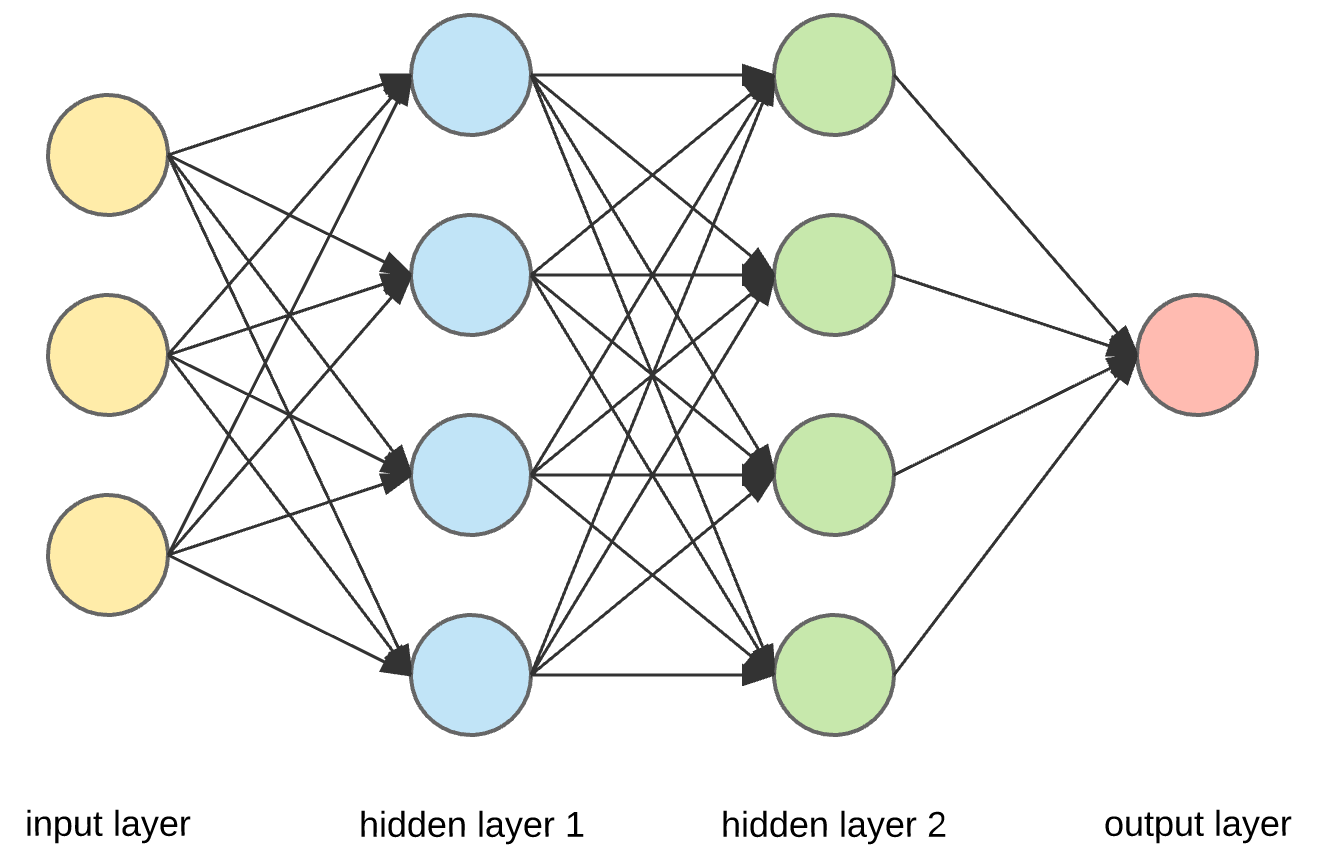
\includegraphics[width=0.75\textwidth]{dnn.png}
\caption{A representation of a deep neural network. The input layer (green) takes the data and feeds it forward in the network to get an output from the output layer (yellow). Each dot represents a neuron, and each line represents the neurons' output computations, including the weight and bias modification as described in \autoref{eq:weightsandbiases} and the activation function.}
\label{fig:dnn}
\end{figure}

To propagate the error modifications through the multiple layers and their non-linear functions, a procedure known as the backpropagation algorithm is used. This procedure utilizes the fact that the gradients for each layer can be seen as applications of the chain rule for derivatives. Specifically, the gradient for a layer in regards to the input of the layer is directly correlated to the gradient for the subsequent layer in regards to the input of that layer. As such, the algorithm can work backwards, first computing the gradient of the output layer and then utilizing that to compute the previous layer's gradient. This makes the algorithm computationally efficient and usable even for large network architectures. \parencite{Goodfellow-et-al-2016} 

Due to the size of deep neural network architectures, training a deep network can be computationally heavy and take up a lot of time. However, the advances in graphical processing units (GPUs) in the last decade have made it possible to greatly speed up the computations required for the learning process, causing convergence to be achieved much faster. \parencite{lecun2015deep}

\subsection{Convolutional neural networks}
One of the drawbacks of a deep neural network as described above, often called a multilayer perceptron (MLP), is that it cannot efficiently handle data input with spatial information, such as two dimensional images. Pixels near each other are important since they contribute to defining features in the image, but an image must be flattened to be input into an MLP. Thus, information that is relevant for features may disappear. 

Convolutional neural networks (CNNs) are a type of neural network that can handle spatial information. A CNN features two different types of layers: convolutional layers and pooling layers. The convolutional layers contain units organized in so called feature maps, where each unit is connected to patches of units in one of the previous layer's feature maps through weight and bias groups called filters. A layer can and often does contain several feature maps, and these use different filters. This architecture causes the local correlation between data points to be kept when going through the layers. The name convolution comes from the name of the mathematical operation performed by the filters. \parencite{lecun2015deep}

The pooling layers are used to pool similar features into one new feature. This can be done in several ways, with one common unit operation being to take the maximum of a patch of units as output. Close by pooling units use patches separate from each other such that the feature maps shrink when going through a pooling layer. \parencite{lecun2015deep}

A convolutional network architecture typically uses these two types of layers together with non-linear activation functions early in the network architecture, and utilizes an MLP network architecture later to extract the approximation of the function value. \parencite{lecun2015deep}

\subsection{Batch normalization}
Batch normalization is a process in which the inputs for each layer of a network are normalized before being used by the layer. This is added as a part of the network architecture, and adds a normalization for each training batch.

The reason for normalizing the inputs is that the distributions of each layer's inputs changes during training since the weights and biases of other layers change. This requires a lower learning rate, which in turn causes learning to be slower. Batch normalization allows for greater learning rates and also makes the network more stable in regards to the initial weight and bias initializations. \parencite{ioffe2015batch}

\subsection{Usage of neural networks}
On their own, neural networks work well for what is known as supervised learning, in which the correct answer is already known beforehand. For instance, when training a network to identify elephants in images, the images trained on are already labelled with whether they contain elephants or not. There are however many problems with no obvious answers. As an example, it is not inherently clear how to optimally play a hole of golf. There are several different actions to choose from, and several steps to take. As such, labelling a golf hole with the suggested actions is a difficult task. Therefore, neural networks on their own cannot successfully be used for problems such as golf. Other methods, such as reinforcement learning, must be used instead.

\section{Related Work}
In this section, articles related to this thesis are presented. Their content and how it relates to this work is described.

Most of the papers referenced in \autoref{sec:reinforcementlearning} are all related to this thesis in that they utilize reinforcement learning algorithms on various problems where the performance can be compared to that of humans. The authors of \parencite{mnih2015human}, \parencite{van2016deep} and \parencite{wang2015dueling} tested their algorithms in the Atari Game environment on several different games, using pixel data as input. The DQN algorithm performed well, setting the state of the art results for Q-learning algorithms and exceeding human level of play in a majority of the games tested. These results were further improved upon in most of the games tested, first by the DDQN algorithm and then even more by the Dueling DDQN algorithm. 

Just like how the discrete algorithms set the state of the art in the discrete action space, the DDPG algorithm performed well in the continuous action space. The algorithm was tested in continuous control environments, such as instances where a robot arm must move an object from one position to another. The results of the algorithm were comparable to or better than that of a planning algorithm, even in cases where the planning algorithm used low-level features while the DDPG algorithm utilized pixel data. \parencite{lillicrap2015continuous}

For hybrid action spaces, the P-DQN algorithm in \parencite{xiong2018parametrized} set the state of the art performance. The algorithm was tested in game environments requiring both continuous and discrete actions, such as the soccer game Half Field Offense (HFO). The performance and speed was further improved by the MP-DQN algorithm in \parencite{bester2019mpdqn}.

In \parencite{vinyals2019grandmaster}, an agent was trained for the immensely complex game StarCraft II. Each game consists of several thousand time steps and in each step, more than $10^{26}$ actions can be chosen. The agent is similar to the one in this paper in that it utilizes human data. However, the agent in \parencite{vinyals2019grandmaster} does it differently in that it uses supervised imitation learning to imitate actions performed by humans. It then uses an actor-critic reinforcement learning method to directly learn a policy that maximizes its win rate. The algorithm performs very well, achieving better results than 99.8\% of StarCraft II players. This is the first algorithm to achieve such a high score.

In \parencite{delalleau2019discrete}, a reinforcement learning algorithm capable of being used in discrete, continuous and hybrid action spaces is presented. This algorithm is based on an actor critic method called Soft Actor Critic (SAC), but modified to work in all types of action spaces. It is therefore named Hybrid SAC. It is compared to the MP-DQN algorithm in the same environments MP-DQN was originally trained on. The results showcased that the Hybrid SAC algorithm performed comparable to, but not better than, the MP-DQN algorithm. The only exception is when the MP-DQN algorithm is simplified for HFO to make the comparison more similar, in which the Hybrid SAC performs better. It was also tested in a Ubisoft game environment in driving a car at high speeds.

The work in \parencite{delalleau2019discrete} showcases a different approach to hybrid action spaces. It is different from the MP-DQN algorithm in that it also can handle discrete and continuous action spaces. This is not necessary in this thesis, which is why the MP-DQN algorithm is preferred.

In \parencite{fu2019deep}, deep multi-agent reinforcement learning is evaluated for hybrid action spaces. Two new algorithms are introduced, the Deep Multi-Agent Parametrized Q-Network (Deep MAPQN) algorithm and the Deep Multi-Agent Hierarchical Hybrid Q-Network (Deep MAHHQN) algorithm. Both of these are based on the P-DQN algorithm. The Deep MAPQN algorithm utilizes P-DQN for several agents, but combines the Q-value outputs into a so called mixing network, to get a total action value for all agents' actions. This is then used to learn how agents can cooperate with each other. This is a quite computationally complex algorithm due to it always having to compute continuous parameters for all discrete actions. The Deep MAHHQN algorithm was therefore implemented to solve this. It uses two networks, one high-level for discrete actions and one low-level for the continuous parameters, that are trained separately. 

Both algorithms in \parencite{fu2019deep} were compared to a group of separate P-DQN agents in several environments, one of them being a multi-agent HFO. In all environments, they performed better than the P-DQN agents. 

The work in \parencite{fu2019deep} relates to this thesis in that it utilizes parametrized reinforcement learning. It is however applied to a vastly different setting, a multi-agent one. This is completely opposite to golf, in which there is no other entity than the agent itself.

\textcite{ArccosGo0:online} is a product that tracks golfers' shots on a golf course using sensors fitted to the golfers' clubs, as well as GPS locations. This data is then used to give recommendations on how to play holes, i.e. which clubs to use. This is similar to one potential use case of the agent from this paper, in that the reinforcement learning agent could be used to showcase how the golfer from which the data was gathered could improve. However, it is unclear whether \textcite{ArccosGo0:online} uses reinforcement learning or any similar method. Furthermore, their data is based solely on club choice and the starting and ending position of the shot. In this paper, entire shots are used to teach the agent, including statistics such as the height and curve of the shot.

\textcite{HelloBir63:online} is a product similar to \textcite{ArccosGo0:online} in that it gives personal recommendations on how to play golf holes. However, \textcite{HelloBir63:online} does not utilize sensors on the golf clubs, and instead uses only GPS data to track golf shots. It is unclear what type of method this product uses for learning.

In \parencite{ko2012simulation}, a model for simulating golf is developed and analyzed to see how different skills, such as long shots, approach shots and putting, in golf affect the final score of a golf round. The golf course model included realistic hole settings, and the golfer shot patterns were modeled using $t$ distributions and normal distributions. The simulations showcased that a 20 yard increase in distance improved the score of high-handicap golfers by almost three strokes, and professional golfers with less than a stroke. They also showcased that the long game accounted for two thirds of the difference in scores between high- and low-handicap golfers.

The work in \parencite{ko2012simulation} is similar to the work in this thesis in that it uses simulation models for simulating golf. However, it differs in that it uses distributions to simulate golf shots, rather than golf shots directly as in this paper. Furthermore, \parencite{ko2012simulation} uses deterministic rules for hitting shots, rather than teaching an agent how to do it. The results show potential use cases for the agent in this paper, i.e. by seeing how differences in a golfer's data affects the agent in its playing.

\chapter{Methods}
\label{chapter:methods}
In this chapter, the methodology of the thesis is detailed. The tools and algorithms used are presented, and the experiments performed are described. 

\section{Golf Simulation Application}
\label{sec:simulation}
In order to train a reinforcement learning agent to play golf, an application simulating a golf environment was needed. This application needed to be able to correctly input golf shots into the environment, handle the physics interactions with objects, make sure the rules of golf were followed, and output observations of the environment to the agent. Furthermore, it was required that the application could run fast enough for training of the agent to be efficient.

The golf simulation application used in this thesis was an application adapted from an application used to play virtual golf games. This virtual golf application fulfilled all requirements mentioned above except for being fast enough for efficient agent training, and being able to output observations for the agent to utilize. This was because the application was used for human consumption, and therefore included a graphical interface. Moreover, the simulation was intentionally slowed down to allow for users to be able to see their shots and results. 

To remedy the speed problems, the virtual golf application was stripped of all graphical components. Furthermore, all logic related to the user interface was also removed. All rules unrelated to the way the agent plays golf, such as rules for playing against other people, were also taken out. Finally, the application speed limitations were removed completely, allowing the application to simulate golf shots and physics as quickly as possible.

Shots close to the green are more complex than longer shots, due to factors such as the height, spin and speed of the shot playing a much bigger role. It was determined that the number of shot types needed in this area could affect the performance of the agents negatively, due to the increased action space complexity. Furthermore, the data required for these types of shots could not easily be gathered. As such, the application was modified to finish a hole as soon as the agent was closer than 30 meters to the hole.

The application was also modified such that it outputted an observation of the environment at the start of each hole and after each golf shot. This observation included the current score of the agent on the hole, whether the hole was completed or not, data about the hole (such as the par of the hole), as well as a two-dimensional map showing the current state of the agent on the hole.

The score of the agents was defined as a penalty dependent on the number of shots hit and the distance remaining to the hole after the hole was finished. More specifically, the score was determined as in \autoref{eq:agentscore}, where $s_n$ is the number of shots hit on the hole, $s_{max}$ is the maximum number of shots for the hole, and $d$ is the distance remaining. As can be seen in the equation, the agent is penalized in intermediary states. Furthermore, the score for final states is normalized depending on the par of the hole. As such, the score of a hole is always between 0 and 1, regardless of the hole's par. Finally, it can be seen that the distance remaining can at most weigh as much as one shot in the final score. As such, the number of shots hit is the more important factor when determining how well the agent performed. 

\begin{equation}
\label{eq:agentscore}
score = 
\begin{cases}
1,& \text{if the hole is not finished or if } s_n = s_{max}\\
\frac{30s_n + d}{30s_{max}},& \text{if } s_n < s_{max}
\end{cases}
\end{equation}

The two-dimensional map was defined such that it contained information on the areas surrounding the current position of the golf ball, with a size of 100x300. The golf ball's position was always at (50,50), and every other cell contained information about the area in a square meter relative to the ball. The golf simulation application always lined up the shot towards a target line, which was either a point in the middle of the fairway or the hole location. This target line was mapped to the north direction in the two-dimensional map. As such, the observation detailed the area 50 meters left and right of the ball, as well as 50 meters behind it and 250 meters in front of it. These numbers were chosen such that the shots gathered would fit in the map, i.e. the agent would have knowledge of where the shots could end up. 

The different types of areas on a hole were mapped to an integer, and these integers were then stored in the map. To see the actual area to integer mappings, see \autoref{app:tab:areamapping} in the appendix. For a visualization of an example of a map, see \autoref{fig:observation}.

\begin{figure}
    \centering
    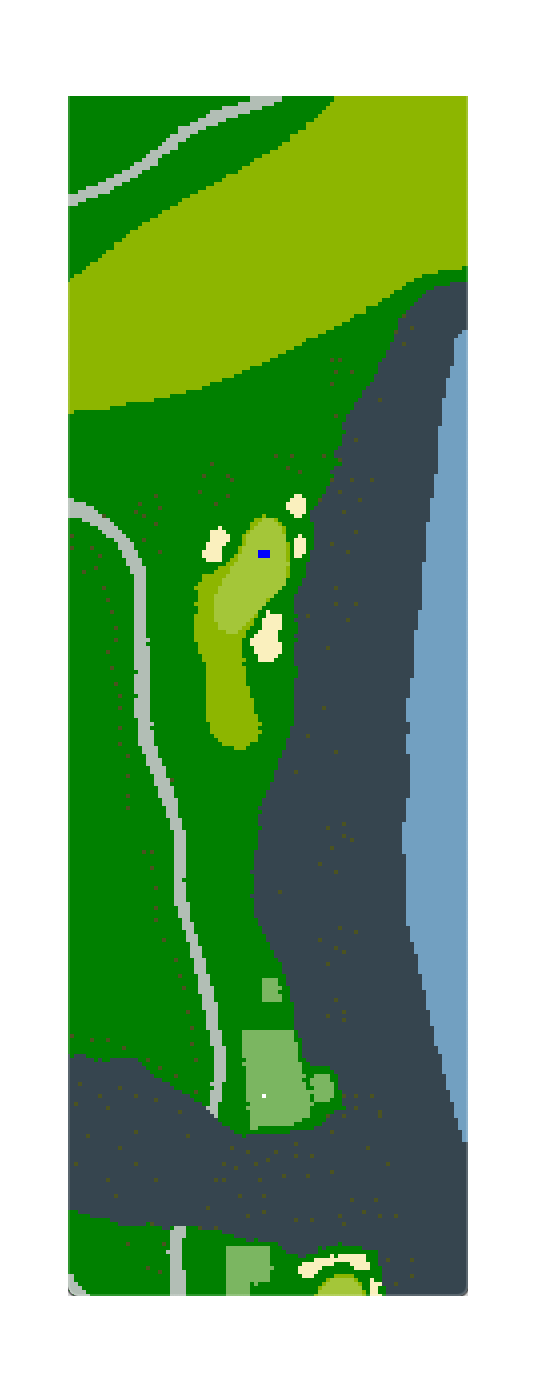
\includegraphics[height=0.5\textheight]{golf_observation_visualization.png}
    \caption{An example visualization of a map from an environment observation. The white dot indicates the ball position, always positioned at (50,50). Specifically, this map showcases the fifth hole at Pebble Beach.}
    \label{fig:observation}
\end{figure}

The reason for not having a larger map was to reduce the time needed for agent calculations, as well as to reduce the risk of learning about holes rather than general positions. This latter reason is also why the ball is always located at the same position in the map.

\section{Shot Data Gathering}
\label{sec:datagathering}
The agents learned to play golf limited by the shot data of a golfer. As such, data was needed for the agents to learn with. This data had to describe the shots well enough such that the agents could use them to approximate the way the golfer plays, and learn from that.

For this thesis, the data included shot data mapped to different clubs. For each club used by the golfer, data from a set of full swing shots hit with that club was gathered. Furthermore, data for a set of shorter distances was gathered as well. These distances were between 30 meters (the lower distance limit of the simulation environment) and the length of the shortest club hit by the golfer, and were added for the agents to be able to learn to play within that distance range as well. More specifically, shots were categorized into the following groups: Driver, 3 Wood, 4 Iron, 5 Iron, 6 Iron, 7 Iron, 8 Iron, 9 Iron, Pitching Wedge, Gap Wedge, Sand Wedge, Lob Wedge, 35 meters, 45 meters, 55 meters and 65 meters. From here on out, these clubs and distances will be abbreviated as in \autoref{tab:clubabbreviations}, and be collectively referred to as clubs.

\begin{table}
    \centering
    \begin{tabular}{c|c}
        \textbf{Club} & \textbf{Abbreviation} \\ \hline
        Driver & DR \\ 
        3 Wood & 3W \\  
        4 Iron & 4I \\  
        5 Iron & 5I \\  
        6 Iron & 6I \\  
        7 Iron & 7I \\  
        8 Iron & 8I \\  
        9 Iron & 9I \\  
        Pitching Wedge & PW \\  
        Gap Wedge & GW \\  
        Sand Wedge & SW \\  
        Lob Wedge & LW \\  
        35 Meters & 35 \\  
        45 Meters & 45 \\  
        55 Meters & 55 \\  
        65 Meters & 65 \\  
    \end{tabular}
    \caption{A table indicating the abbreviations utilized for the various clubs and distances that were used during the shot data gathering.}
    \label{tab:clubabbreviations}
\end{table}

It was possible to gather data through the use of a camera based ball tracking system, which could pinpoint golf shot positions in three dimensions over time while they were being hit. This data generated by the system was stored, along with values regarding the ball flight, such as the total distance, the launch angle, and speed of the ball. 

The shot data used was gathered from a single golfer. This was done because the agents' purpose was to learn how to play golf like a golfer, and having more than one golfer's data does not correctly represent this behaviour. Moreover, when the data was gathered, the golfer was told to aim every shot in the same direction. This was because the agents were supposed to learn how to introduce directional changes itself. By having all shots aimed in the same direction, the misses of the golfer could correctly be gathered. As such, the agents had to take those misses into consideration when learning to play golf.

The data was gathered using a modified version of an application used for visualizing golfers' shots. This application allowed players to choose which club they were hitting and see various statistics regarding the shots from that club. The application was modified such that instead of simply visualizing the data, it permanently stored it to file so that it could be used later. Furthermore, the application was changed such that it randomly selected a club to be hit by the golfer, compared to the golfer choosing themselves. This was done to eliminate bias in choosing clubs. For instance, using the same club two times in a row will most likely cause the second shot to become better because of the golfer feeling the imperfections from the first shot and adapting their swing.

Shot data was gathered during five different occasions to reduce the bias from the daily form of the golfer. For each club, 8 shots were gathered per occasion, resulting in a total of 40 shots per club. This number was seen as enough to approximate each type of shot well enough, while still being within the time frame available for this thesis. 

In order to evaluate the agent's performance, data was also needed of the golfer playing golf. As such, data from different rounds of golf played by the golfer was recorded. Specifically, the same variables required to calculate the scores of the agents were saved, i.e. the number of shots hit and the distance remaining when closer than 30 meters to the hole. The club choices of the golfer were also gathered. This data was gathered using the unmodified virtual golf application and was gathered during the same occasions as the rest of the data. This was done to reduce the risk of the golfer's performance having changed over time. 

Round data was gathered from the first 9 holes of two different golf courses. Data for five rounds of golf were stored for the first course, Pebble Beach, and four rounds for the second course, Ullna GC. The reason for this difference was due to a lack of time during one of the data gathering occasions.

\section{Reinforcement Learning Agents}
To answer the question posed in \autoref{chapter:introduction}, reinforcement learning agents capable of observing the golf environment and selecting actions for hitting golf shots were required. Two types of deep reinforcement learning agents were implemented and evaluated for this purpose: a Dueling DDQN agent and a modified version of the MP-DQN agent.

The Dueling DDQN agent utilized, as described in \autoref{chapter:background}, a dueling network layer in conjunction with a Double Deep Q network to determine club choices given observations. Since this algorithm only deals with discrete action spaces, the Dueling DDQN agent could not handle choosing a direction to hit in, but focused only on the club choices. This might sound suboptimal for the problem, but the agent was implemented to discover how important of a factor the direction was, both in terms of an agent's performance in playing golf and in terms of how well an agent learns depending on the problem's complexity. 

The Dueling DDQN agent utilized the same network structure as in \parencite{wang2015dueling}. That is, it contained the same number of neurons, and utilized the same activation and learning functions. Moreover, it also used the $\epsilon$-greedy policy for exploration.

The MP-DQN agent differed from the one presented in \parencite{bester2019mpdqn}. In the original version, the dueling network layer was omitted in order to make comparisons between algorithms fair. Since the layer was present in the P-DQN algorithm in \parencite{xiong2018parametrized}, it was also present in the agent used in this thesis. 

The original MP-DQN agent was evaluated on problems in which the state space contained no spatial information. As such, no convolutional layers were needed. The observations in this thesis did include this kind of information and therefore the MP-DQN agent in this paper was modified to include convolutional layers. The policy networks were structured as in the DDPG algorithm in \parencite{lillicrap2015continuous}. For the Q networks, almost the same structure of convolutional layers as in the Dueling DDQN algorithm was used. Since the Q networks also used the action parameters as input, and since these parameters contained no spatial information, the parameters were not added as input to the convolutional layers. Instead, they were combined with the extracted features from the convolutional layers and input into the remaining network structure.

The agents learned by playing holes of golf, where one hole was defined as an episode. First, the agents received an initial observation from the environment (as defined in \autoref{sec:simulation}), showcasing the starting position on the hole. The two dimensional map from this observation was input into the agents' networks and the Q-values for the actions (as well as their corresponding parameters for the MP-DQN) were received as output. Then, the agents chose the corresponding actions according to the $\epsilon$-greedy policy, which were converted into a shot that was input to the simulation environment. The environment then returned the next observation, which as mentioned contained the new position on the hole, whether the hole was finished, as well as the penalty the agent received. Finally, the agents performed network learning updates using their experience replays. This procedure was repeated until the hole was finished. The information from the episode was then stored and a new episode was started. This information included which hole was played, what par the hole had, the number of shots hit, the distance remaining to the hole after the hole was finished, the penalty received, the club choices, and the directional choices.

For the Dueling DDQN agent, the corresponding actions to an observation included choosing which club to hit. From this choice, one of the golfer's gathered shots with that club was uniformly sampled. This shot was then hit in the direction of the target line in the simulation environment.

For the MP-DQN agent, the same club choice as with the Dueling DDQN agent was performed. However, this choice also included a continuous parameter; the directional deviation from the target line. This was a value between -20 and 20 degrees. Before the sampled shot was input into the simulation environment, it was rotated to be hit in the chosen direction. The deviation limits were added to minimize the complexity of the state space, while still allowing deviations that were reasonable in terms of how a golfer would play a hole.

For both agents, the club choice was actually variable; all actions were not available in all states. Specifically, the DR could not be used on any other shot except the first one on each hole. This was because the DR is a club which in most cases is only used when the ball is elevated from the ground using what is known as a tee, and the tee can only be used on the first shot of a hole. For all shots gathered with the DR a tee was used, making shots hit with the club illegal if they were not the first on a hole.

To handle the above mentioned problem, the agent was punished more if it chose the DR when a shot had already been hit on a hole. Specifically, the agent got a punishment of $1.1$ and returned to the same state it currently was in. 

\subsection{Training}
\label{sec:rltraining}
The agents were trained on two different course configurations. The first configuration contained the first nine holes of the course Pebble Beach, and the second contained the first nine holes of the course Ullna GC. This was because the purpose of this thesis is to investigate how well the agents compare to the golfer, and as such the configurations only contained the holes data was gathered from. This might have affected the agents in their ability to play golf in general, a topic which is touched upon in \autoref{chapter:discussion}.

Both agents were trained on both configurations. During training, holes from the configurations were played at random, and the best weights were saved. These weights were determined by keeping the penalties of the last 100 par 3 holes, the last 100 par 4 holes as well as the last 100 par 5 holes, and taking the average of these penalties. The weights that caused the lowest average penalty were stored as the best.

Although the simulation application was sped up, the time required for training the agents was quite long. Due to the time limitations on this project, no extensive hyperparameter tests could be conducted. Instead, the parameters used in the original Dueling DDQN and DDPG algorithms were used as a baseline, and a few combinations of parameters were tested using the parameters in \parencite{bester2019mpdqn} as guidelines. Specifically, the learning rates of the networks, the rate at which $\epsilon$ decreased and the number of episodes were tuned. For the policy networks in the MP-DQN agent, $10^{-4}$, $10^{-5}$ and $10^{-6}$ were tested. For the Q networks, $10^{-3}$, $10^{-4}$ and $10^{-5}$ were tested. The number of episodes varied between $10000$ and $200000$. For the rate at which $\epsilon$ decreased, $10^{-4}$, $10^{-5}$ and $2 \cdot 10^{-6}$ was tested. The values used in the final tests can be found in \autoref{tab:hyperparameters}. As can be seen in the table, some other values differed from the literature on which the agents were based. These values were changed due to the reduced time available for training compared to the original algorithms' training times.

\begin{table}
    \centering
    \begin{tabular}{c|c}
        \textbf{Hyperparameter} & \textbf{Value} \\ \hline
        Episodes & $50000$ \\ 
        Q Network learning rate & $10^{-4}$ \\ 
        Policy Network learning rate & $10^{-5}$ \\ 
        $\tau$ & $10^{-3}$ \\ 
        $\epsilon_{min}$ & $0.02$ \\ 
        $\epsilon_{dec}$ & $10^{-5}$ \\ 
        Batch size & $32$ \\ 
        Experience Replay size & $10000$ \\ 
        Q Target network replacement iterations & $1000$ \\ 
        $\gamma$ & $0.99$ \\
    \end{tabular}
    \caption{A table showing the hyperparameters used for the final tests of the agents.}
    \label{tab:hyperparameters}
\end{table}

The agents were both trained and evaluated on a computer using 16GB of RAM as well as an NVIDIA GeForce GTX 970 graphics card. The GPU was utilized both for the training of the networks and the golf simulation application. The experience replay was always stored in memory during training. The agents were implemented in Python, with PyTorch and NumPy used as machine learning libraries. The network structures and experience replay were implemented as their own classes, and these components were then used to create agent classes. The agent classes then communicated through an API with the golf simulation application.

\subsection{Evaluation}
The agents were evaluated on the same configurations they were trained on, one containing the first nine holes of Pebble Beach and one containing the first nine holes of Ullna GC. They were evaluated by playing 5000 random holes on their respective course. The results from these holes were stored and analyzed on the score, the number of shots hit, the distance remaining to the pin, the club selections and the directional deviations chosen.

During the evaluation, no noise was added to the policy network output, and no exploration was done by any agent in order to see what the agents had learned. Because of this, the agents could end up in an endless loop of trying to choose the DR club when in a state that did not allow it. Therefore, the DR club choice was redirected to the closest legal club choice, the 3W, when chosen in an illegal state during evaluation.

To determine how well the agents played compared to the golfer from which the data was gathered from, 250 samples of each hole from Pebble Beach and Ullna GC were retrieved from the results of the 5000 holes played, and the scores were compared to the samples gathered from the golfer. Finally, statistical significance tests were performed to determine if the agents played better than, worse than, or on the same level as the golfer.

\chapter{Results}
\label{chapter:results}
In this chapter, the results from the experiments mentioned in \autoref{chapter:methods} are presented. The numbers are explained, and graphs and tables are used to visualize the outcomes of the tests.

\section{Shot Data}
This section details the results from the data gathering process of the thesis. The shot data retrieved from the golfer used by the agent is presented, including numbers describing the shots.

As was described in \autoref{sec:datagathering}, 40 shots were gathered for each club. \autoref{fig:all_shots} showcases the landing positions for all shots, colour coded on the club used. Figures for the shots grouped by club can be found in \autoref{app:shot_data}. In the figures, the axes' numbers are in meters. As can be seen, the X-axis goes from right to left. This is because of the coordinate system used in the application used for gathering the data. It is shown in the figures that the shots covered essentially all distances between the shortest shot and the longest. Furthermore, the shots were generally straight, with the shorter clubs or distances being less spread out than the longer ones.

\begin{figure}
    \centering
    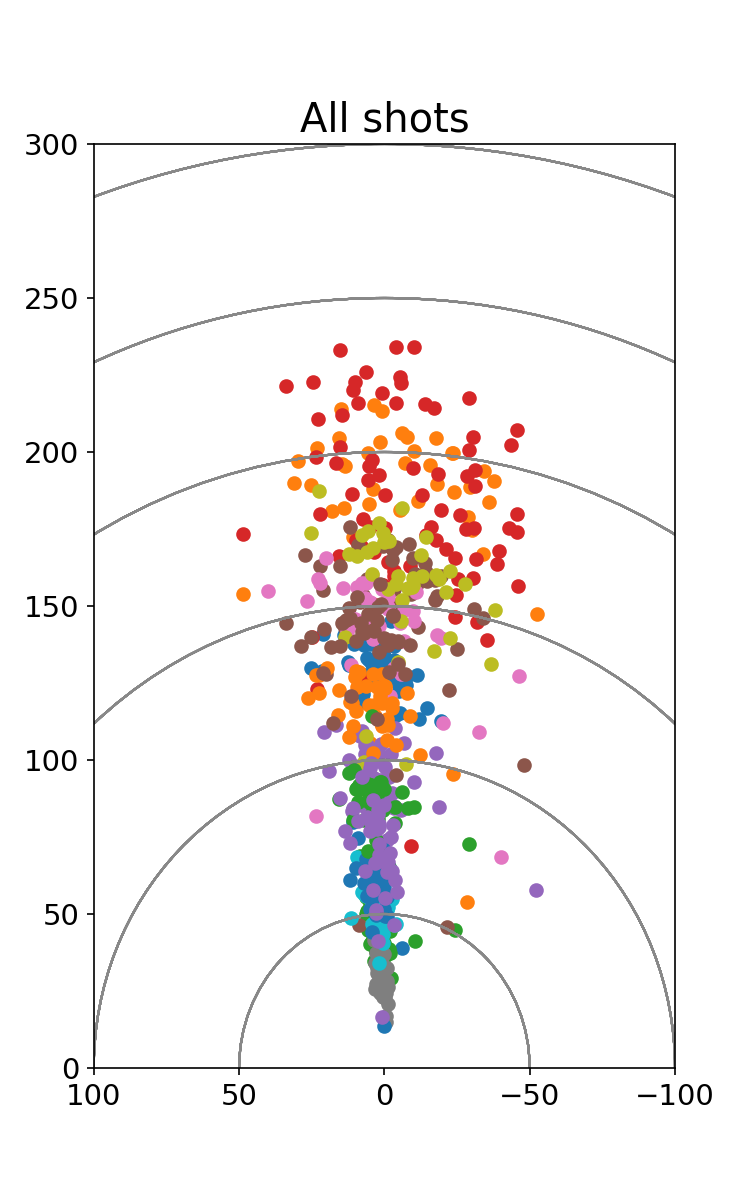
\includegraphics[height=0.4\textheight]{Shots/all_shots.png}
    \caption{The landing positions of all shots gathered from the golfer. The axes show the distance in meters. All shots of the same color were hit with the same club. The contours show the distances from the starting position with a 50 meter interval.}
    \label{fig:all_shots}
\end{figure}

In \autoref{fig:shot_data_distance}, boxplots showcasing the carry distances for each club are presented, where carry distance is defined as the distance between the starting point and the landing point of a shot. In \autoref{fig:shot_data_angle}, boxplots for the offline angles for each club are presented. That is, the angles between the target line and the landing position of the shots are shown.

\begin{figure}
    \centering
    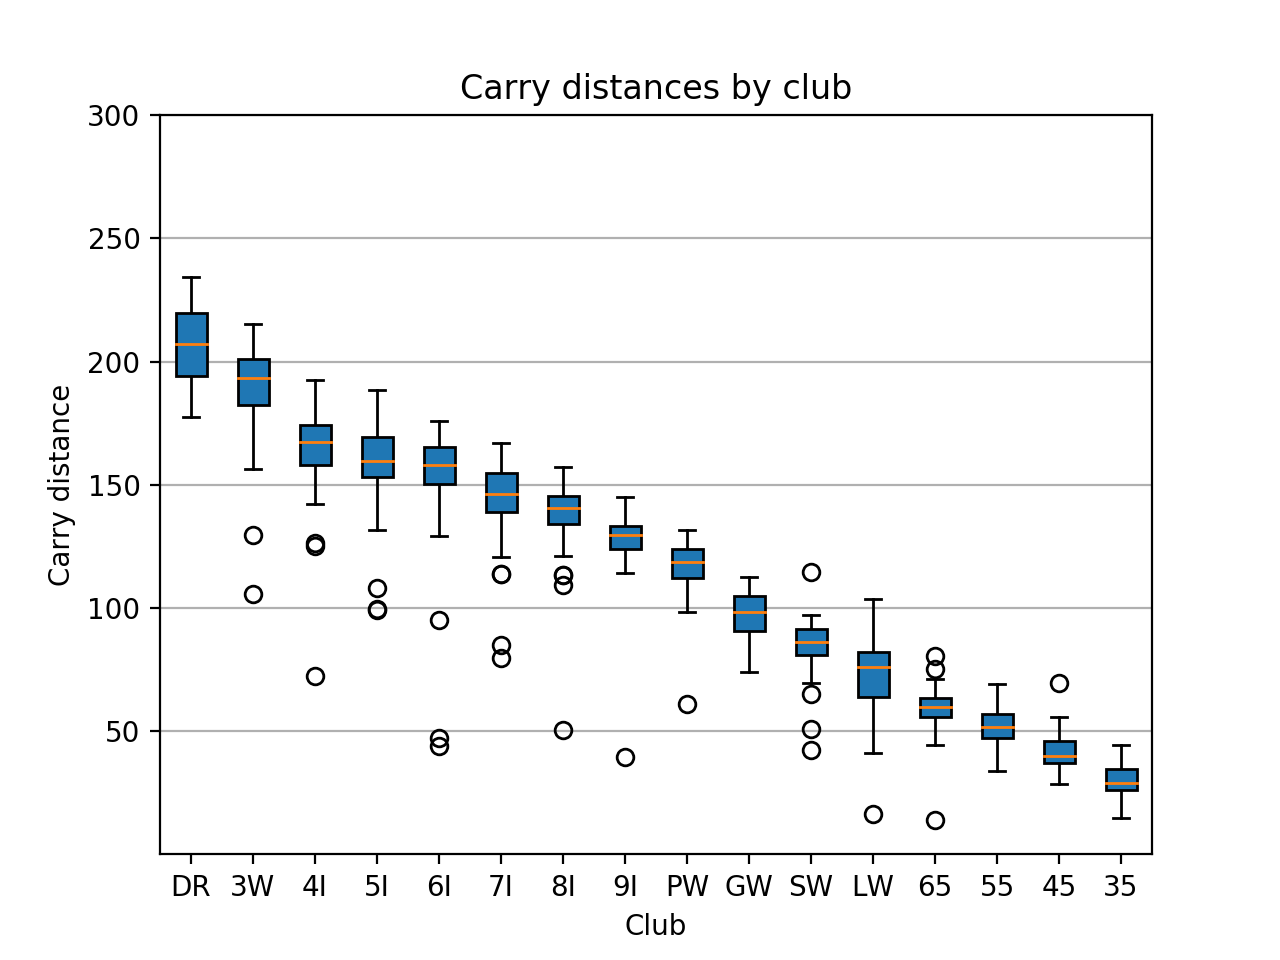
\includegraphics[width=0.5\textwidth]{Boxplots/distances.png}
    \caption{Boxplots showcasing the carry distances for each club hit by the golfer.}
    \label{fig:shot_data_distance}
\end{figure}

\begin{figure}
    \centering
    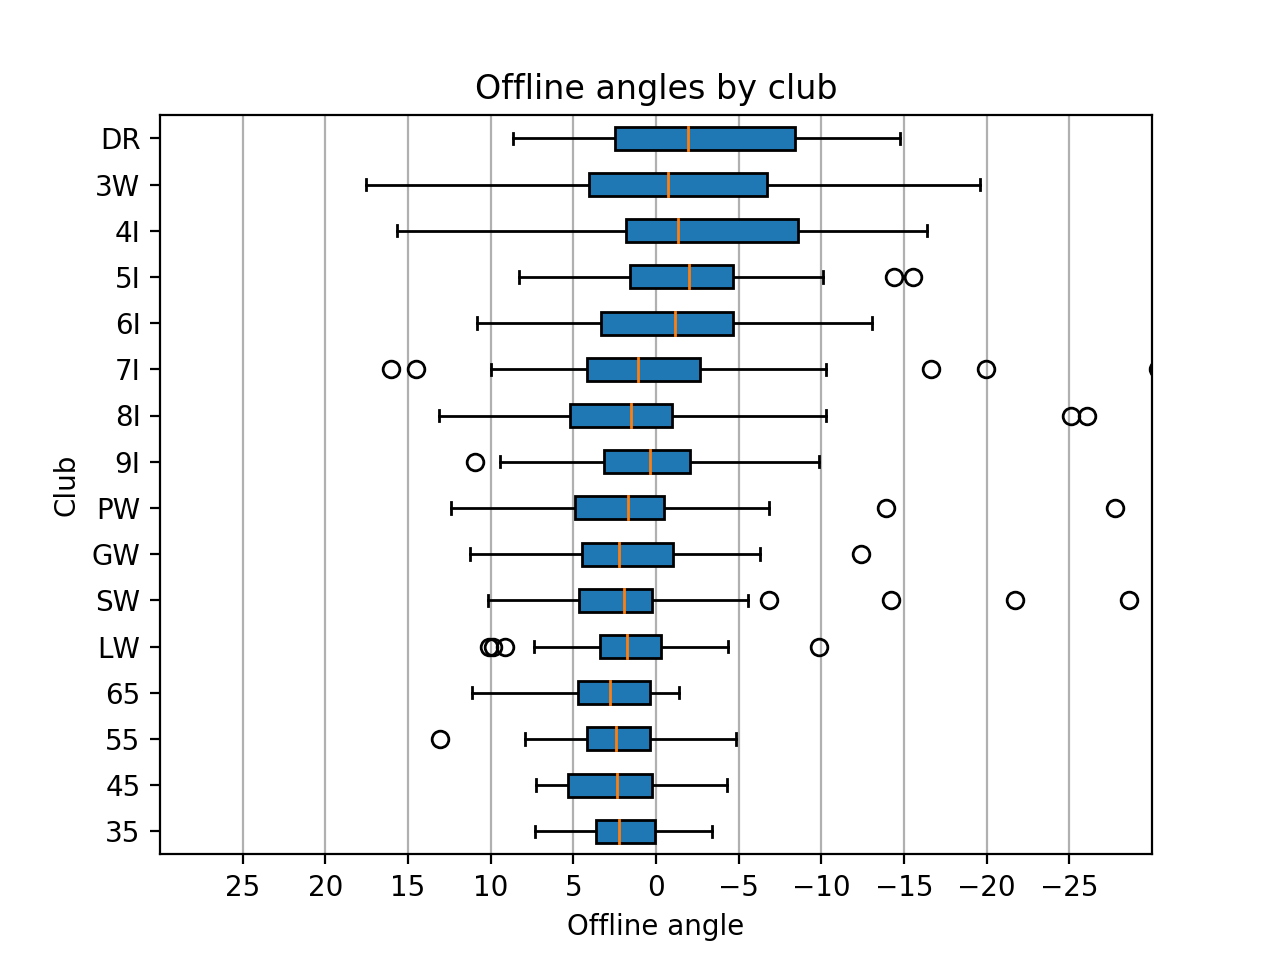
\includegraphics[width=0.5\textwidth]{Boxplots/directions.png}
    \caption{Boxplots showcasing the offline angles for each club hit by the golfer. That is, the angles between the landing position of the shot and the target line are presented.}
    \label{fig:shot_data_angle}
\end{figure}

The plots in \autoref{fig:shot_data_angle} also indicate that most shots were generally hit straight, since the average offline angles were lower than 3 in any direction. However, the minimum and maximum values show that some clubs had a big spread, for instance the 3W. This shows that the agents can end up in states that differ much, even though the same club has been used. It is also interesting to note that the shorter clubs and distances all have a positive average offline angle, whereas the longer clubs all have a negative angle.

The same analysis can be derived from the values in \autoref{fig:shot_data_distance}. The average shot distances gradually increase from the shortest to the longest club used. The minimum and maximum values showcase however that the distance can fluctuate much for a club. For instance, the shortest and longest 6I shot differed around 130 meters in carry distance. 

It is important to note that the plots in the above mentioned figures do not take into account how much the balls bounced and rolled after landing. This data was excluded from the graphs in this section due to it being dependent on the terrain where the shot lands.

\section{Golfer and Agent Comparison}
In this section, the results from training and evaluating the reinforcement learning agents are presented. Furthermore, the golfer's results on the courses played are showcased and compared to the agents' results. The agents' training progress is showcased, and the results on the holes evaluated are detailed. The choices made by the agents and the golfer are also described. From here on out, the term score refers to the score function utilizing the number of shots hit on a hole and the distance remaining to the hole, as described in \autoref{eq:agentscore}.

\subsection{Training}
In \autoref{fig:training_plots}, the learning progress of each agent on each training configuration is presented, using rolling averages of $500$ episodes. That is, the average score of the $500$ previous episodes is used for each data point in the plots. In the figure, it is shown that all agents were capable of learning to play golf during training. Specifically, all agents lowered their average score to between $0.3$ and $0.4$ during the training process. However, due to the training process always including some exploration, this is not indicative of how well the agents played.

\begin{figure}
    \centering
    \begin{subfigure}{0.45\textwidth}
    \centering
    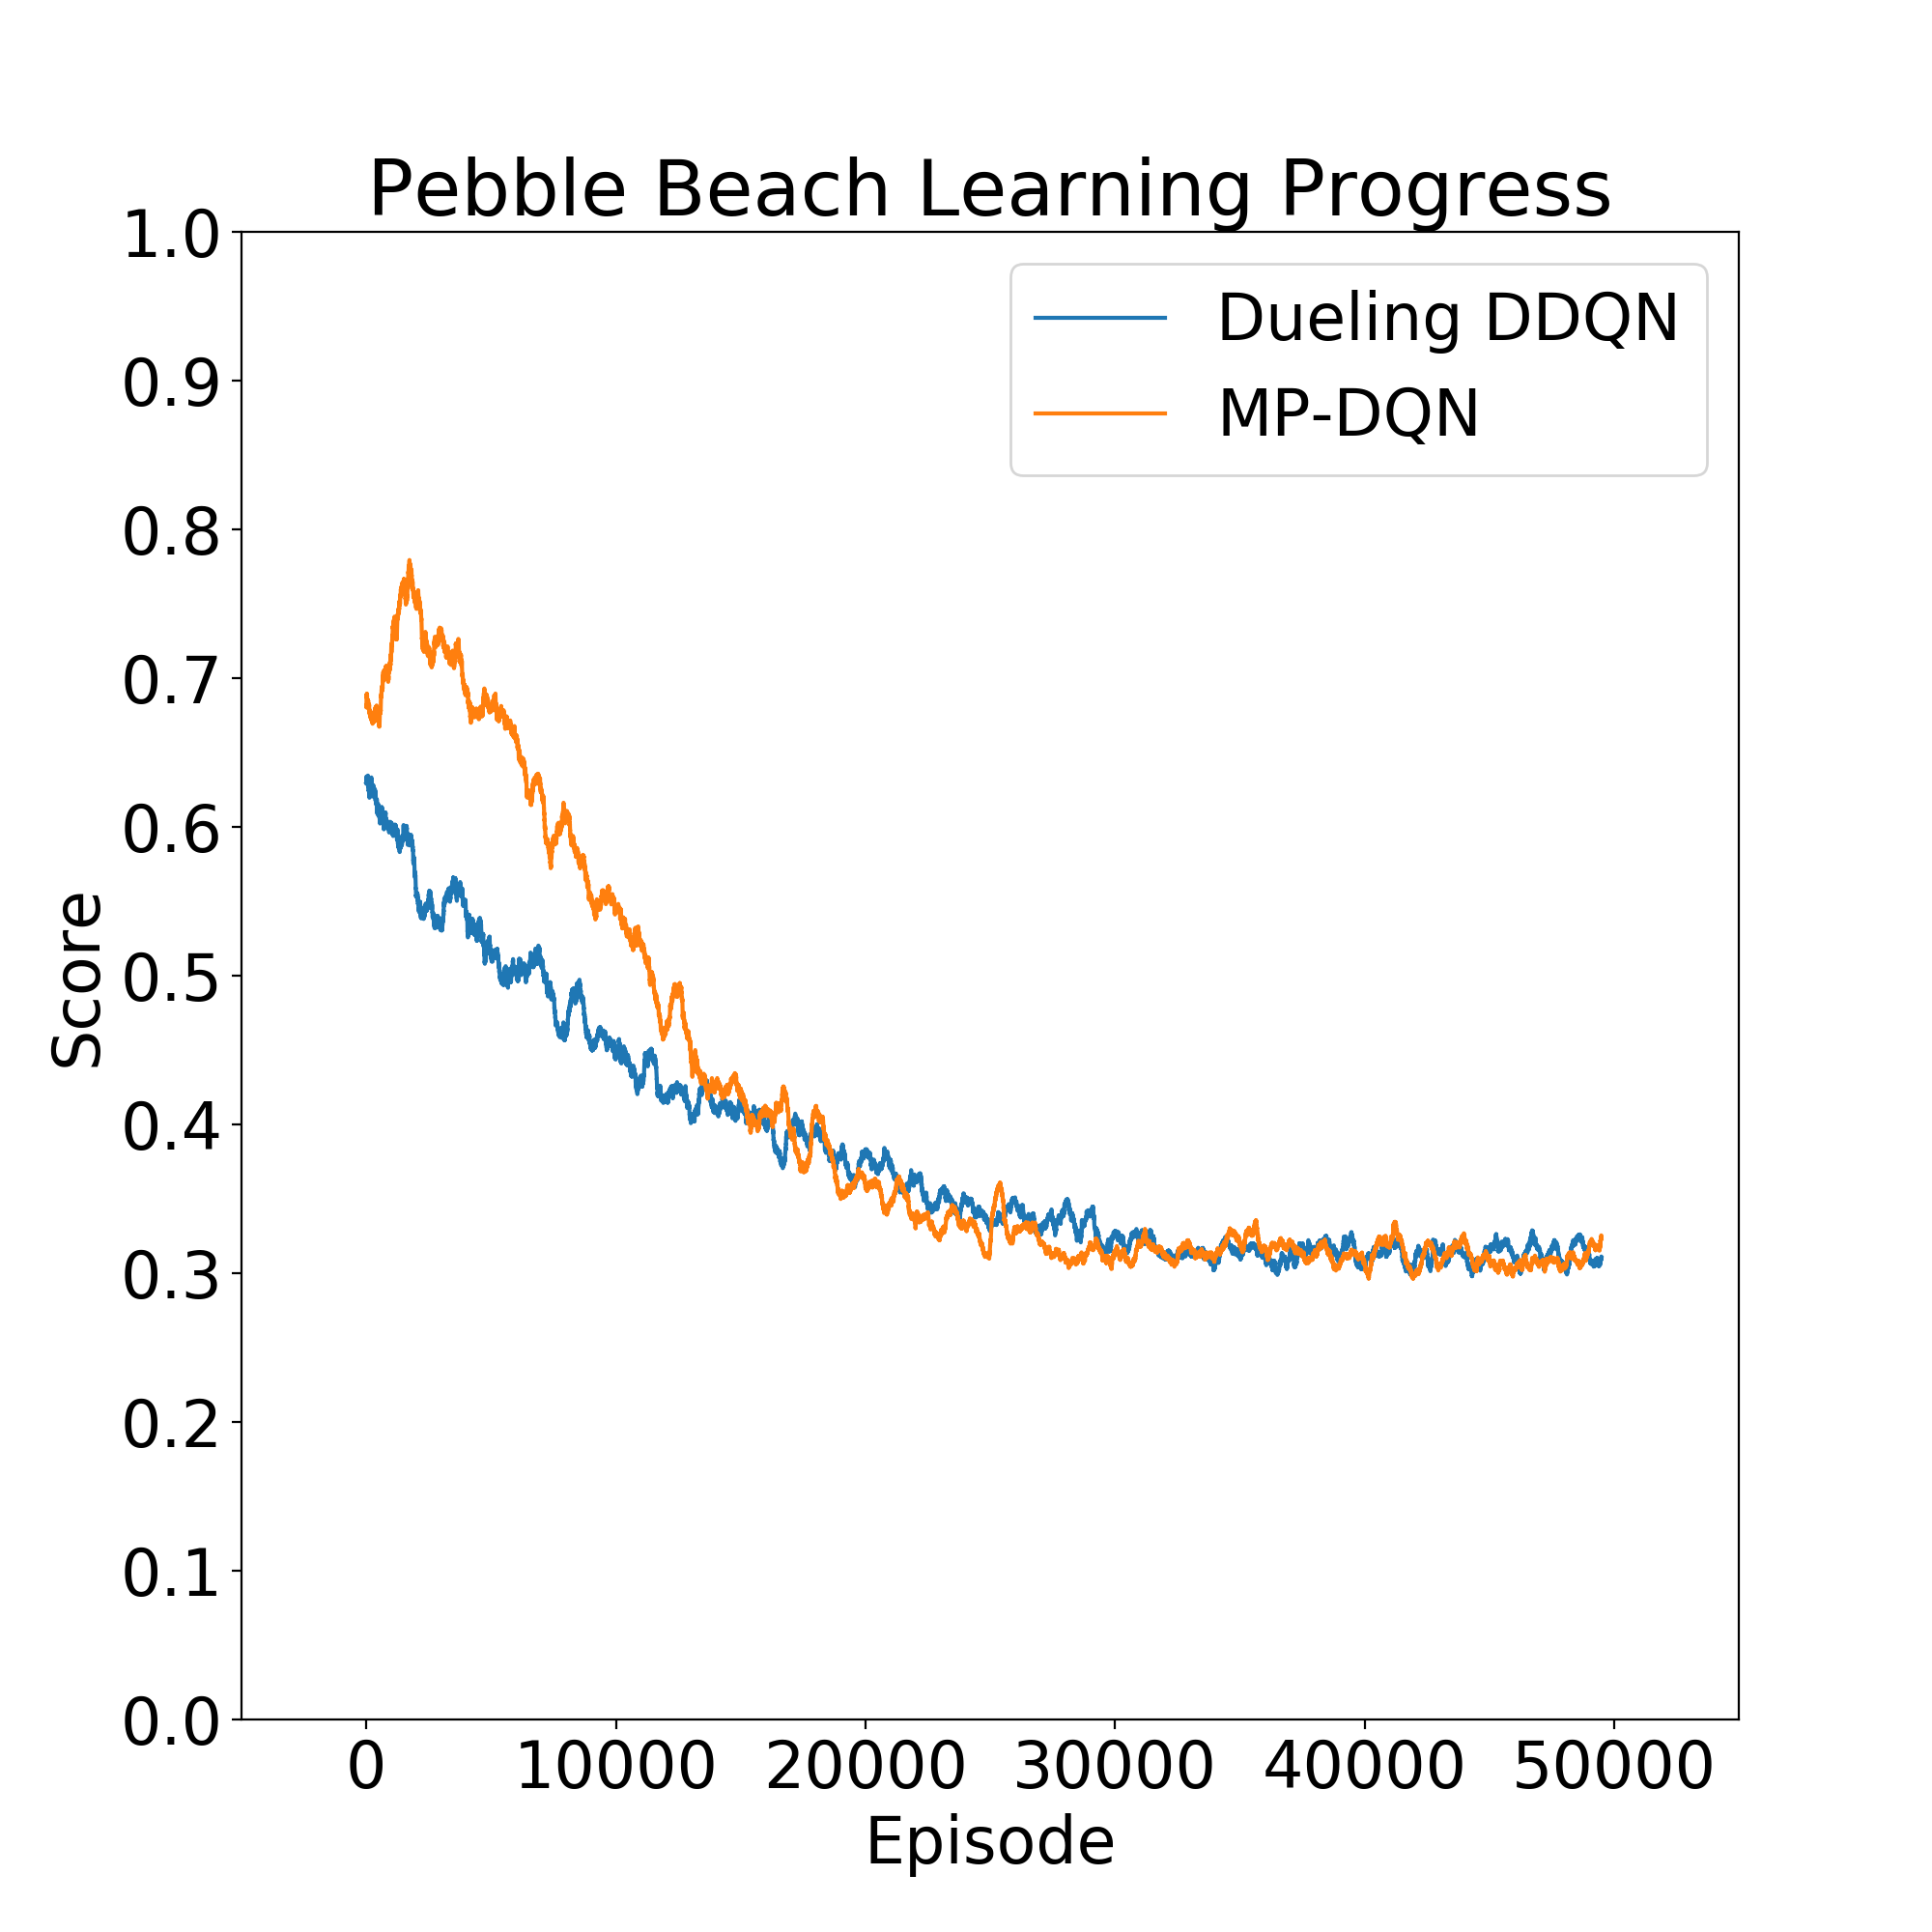
\includegraphics[width=\textwidth]{TrainingPlots/Pebble9_training.png}
    \end{subfigure}
    \begin{subfigure}{0.45\textwidth}
    \centering
    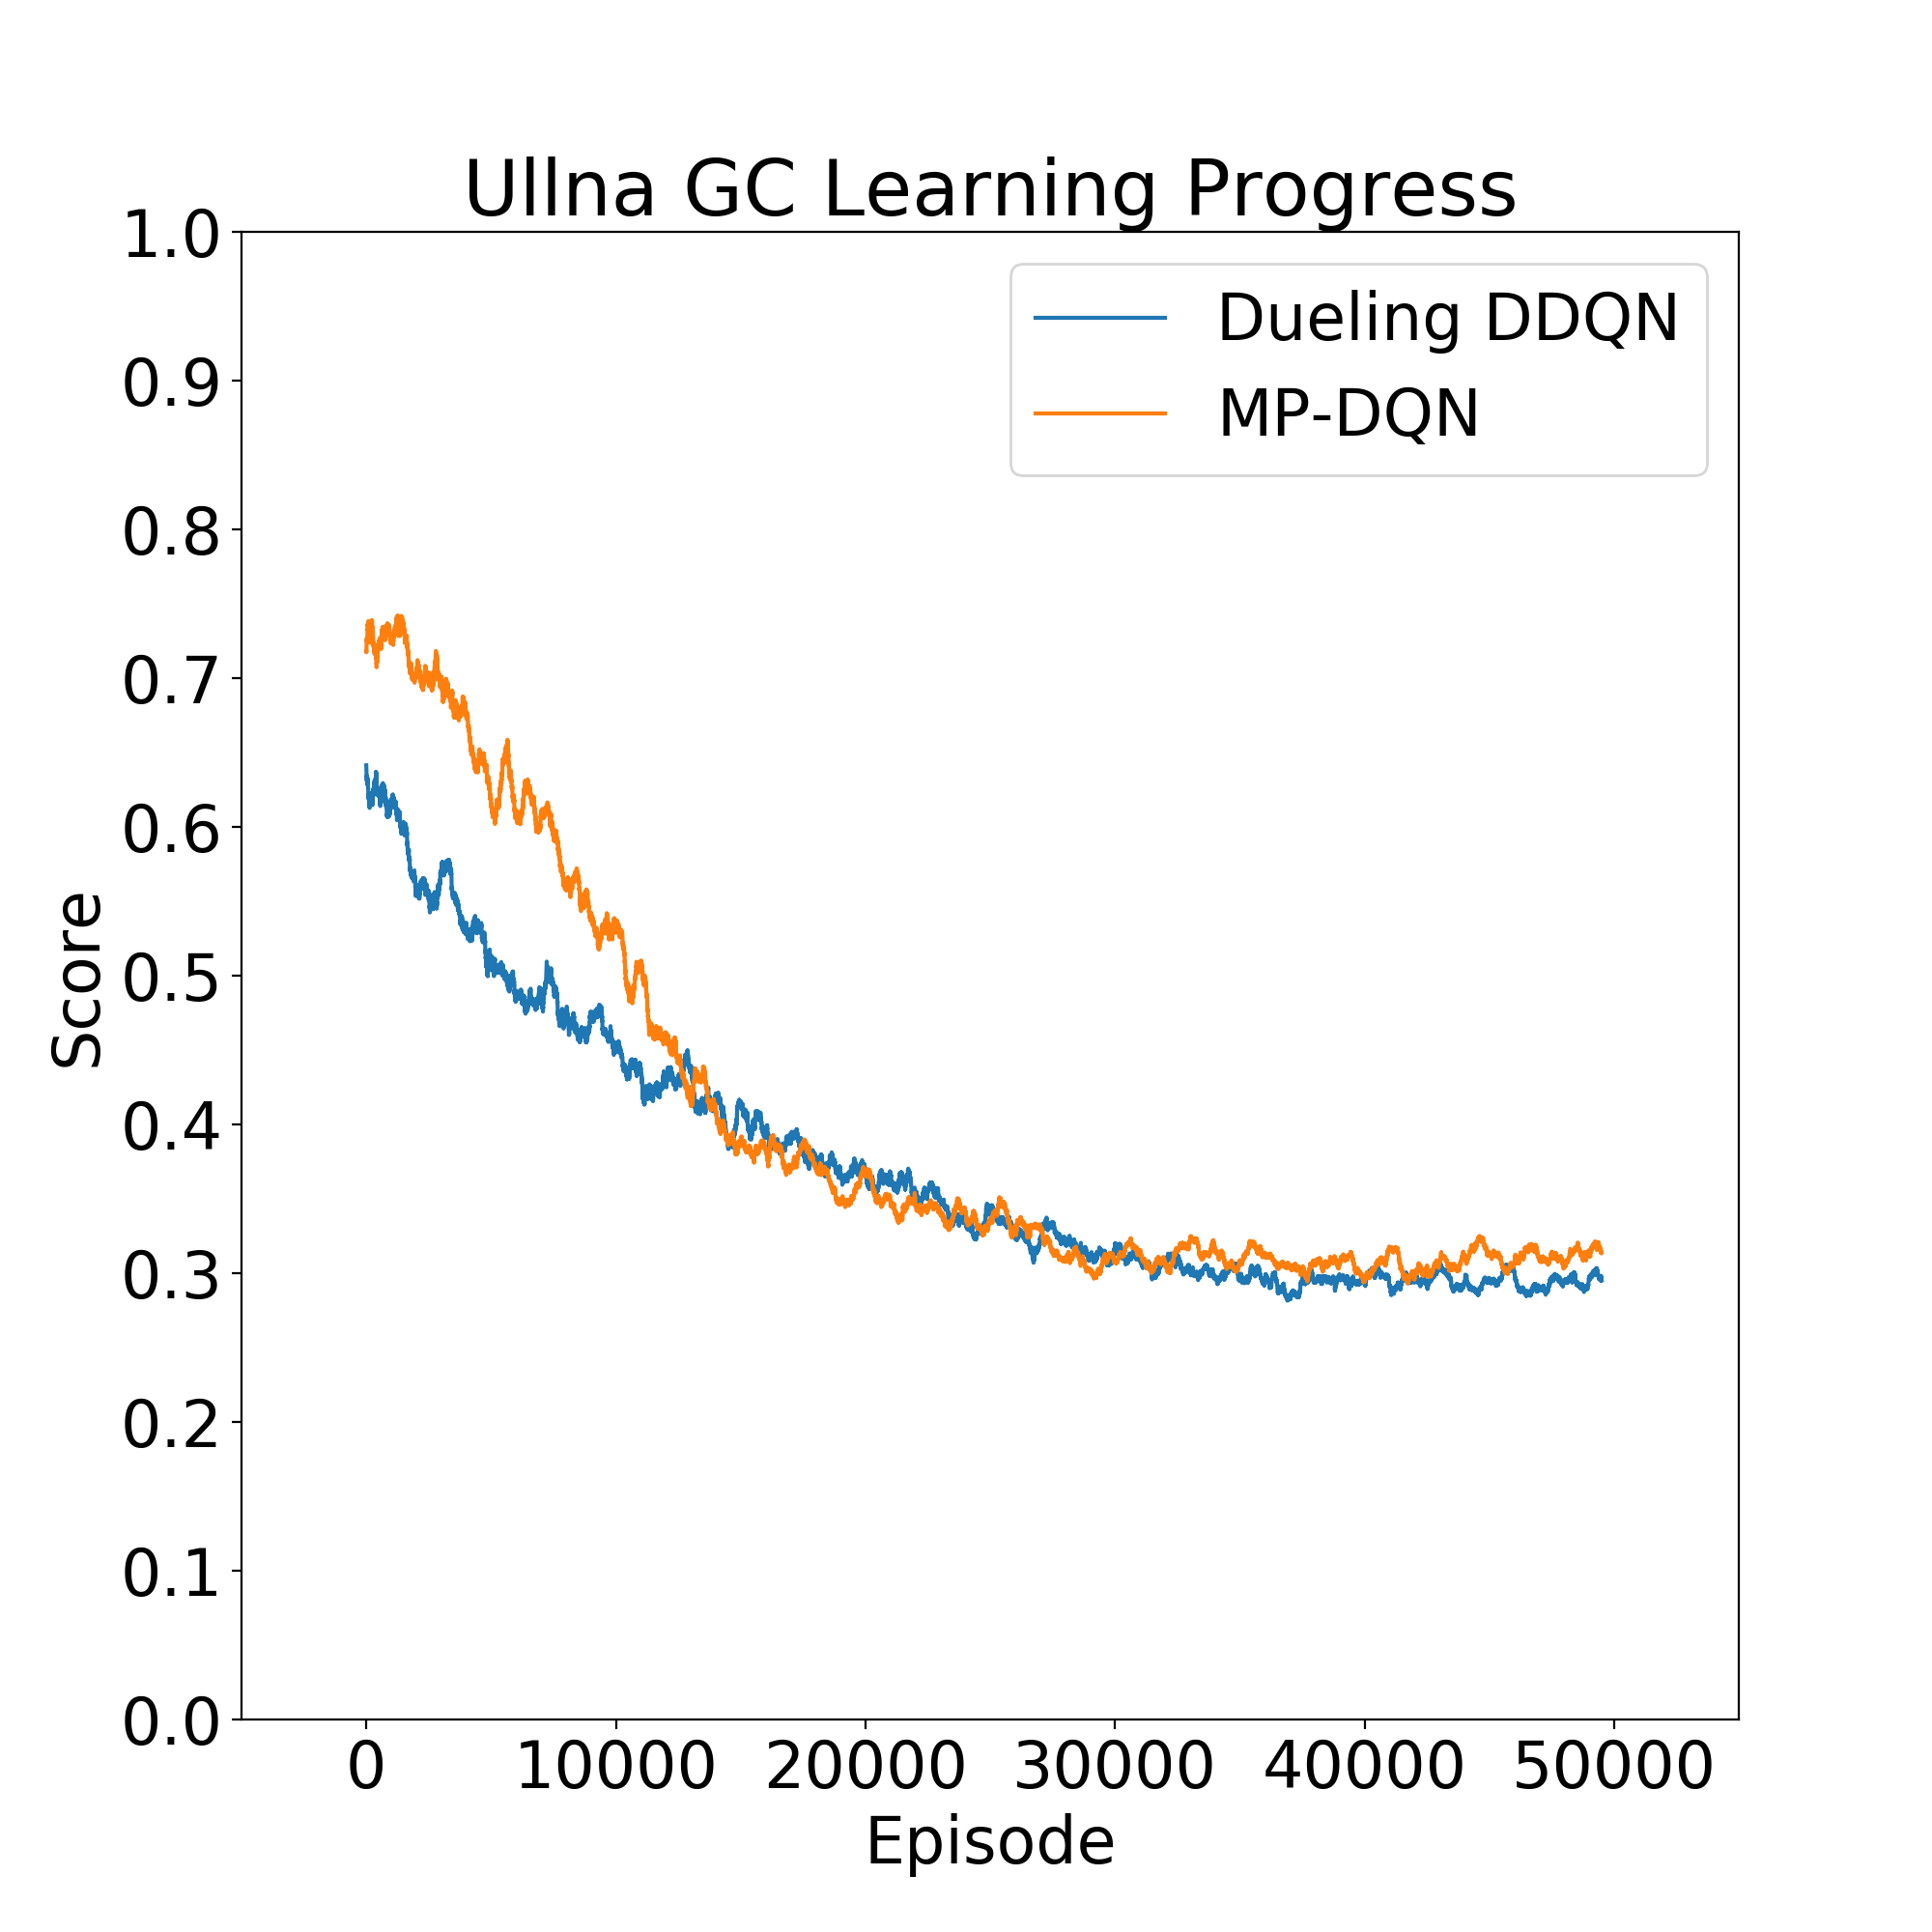
\includegraphics[width=\textwidth]{TrainingPlots/Ullna9_training.png}
    \end{subfigure}
    \caption{The rolling averages over 500 episodes of scores for the two training configurations. Each subfigure contain plots for both the Dueling DDQN agent and MP-DQN agent.}
    \label{fig:training_plots}
\end{figure}

\subsection{Evaluation}
The results in this subsection are divided into two groups; Pebble Beach results and Ullna GC results. For each group, the golfer's results, as well as the agents' performances and their club choices and directional deviations are presented.

\subsubsection{Pebble Beach}
In \autoref{tab:pebble_average_results}, the average scores, number of shots and distances remaining for each hole on Pebble Beach are presented for the golfer, the Dueling DDQN agent and MP-DQN agent. As was mentioned in \autoref{chapter:methods}, the golfer was evaluated over five rounds, whereas the agents were evaluated over 250 rounds. The tables showcase that both the golfer and the agents found some holes more difficult than others. This is also true when comparing the Dueling DDQN and MP-DQN agents. For instance, the Dueling DDQN agent performed better than the MP-DQN agent on hole 2, but the opposite was true for hole 6.

\begin{table}
    \begin{subtable}{\textwidth}
    \centering
    \begin{tabular}{c|c|c|c|c}
    \multicolumn{5}{c}{\textbf{Pebble Beach Average Golfer Results}} \\ 
        \textbf{Hole} & \textbf{Par} & \textbf{Score} & \textbf{Shots} & \textbf{Distance remaining (m)}  \\ \hline
        1 & 4 & 0.31 & 2.20 & 17.60 \\ 
        2 & 5 & 0.31 & 2.80 & 8.82 \\ 
        3 & 4 & 0.27 & 2.20 & 7.00 \\ 
        4 & 4 & 0.32 & 2.60 & 7.30 \\ 
        5 & 3 & 0.18 & 1.00 & 12.18 \\ 
        6 & 5 & 0.35 & 3.00 & 15.00 \\ 
        7 & 3 & 0.21 & 1.20 & 15.04 \\ 
        8 & 4 & 0.32 & 2.60 & 7.76 \\ 
        9 & 4 & 0.29 & 2.20 & 11.28 \\
    \end{tabular}
    \end{subtable}
    \hfill
    \begin{subtable}{\textwidth}
    \centering
    \begin{tabular}{c|c|c|c|c}
    \multicolumn{5}{c}{\textbf{Pebble Beach Average Dueling DDQN Results}} \\ 
        \textbf{Hole} & \textbf{Par} & \textbf{Score} & \textbf{Shots} & \textbf{Distance remaining (m)}  \\ \hline
        1 & 4 & 0.30 & 2.26 & 12.76 \\ 
        2 & 5 & 0.30 & 2.48 & 14.16 \\ 
        3 & 4 & 0.29 & 2.14 & 12.76 \\ 
        4 & 4 & 0.34 & 2.62 & 12.75 \\ 
        5 & 3 & 0.19 & 1.12 & 11.70 \\ 
        6 & 5 & 0.51 & 4.64 & 17.26 \\ 
        7 & 3 & 0.20 & 1.30 & 9.91 \\ 
        8 & 4 & 0.34 & 2.56 & 15.36 \\ 
        9 & 4 & 0.35 & 2.62 & 16.37 \\ 
    \end{tabular}
    \end{subtable}
    \hfill
    \begin{subtable}{\textwidth}
    \centering
    \begin{tabular}{c|c|c|c|c}
    \multicolumn{5}{c}{\textbf{Pebble Beach Average MP-DQN Results}} \\
        \textbf{Hole} & \textbf{Par} & \textbf{Score} & \textbf{Shots} & \textbf{Distance remaining (m)}  \\ \hline
        1 & 4 & 0.30 & 2.22 & 15.19 \\ 
        2 & 5 & 0.31 & 2.62 & 15.09 \\ 
        3 & 4 & 0.30 & 2.17 & 14.70 \\ 
        4 & 4 & 0.30 & 2.24 & 13.43 \\ 
        5 & 3 & 0.21 & 1.12 & 17.54 \\ 
        6 & 5 & 0.39 & 3.40 & 15.75 \\ 
        7 & 3 & 0.19 & 1.11 & 13.04 \\ 
        8 & 4 & 0.35 & 2.61 & 16.53 \\ 
        9 & 4 & 0.35 & 2.60 & 16.97 \\ 
    \end{tabular}
    \end{subtable}
    \caption{The average scores, number of shots and distances remaining gathered from the golfer, Dueling DDQN agent and MP-DQN agent for each hole on Pebble Beach, respectively. All numbers are rounded to two decimals.}
    \label{tab:pebble_average_results}
\end{table}

When looking at the average scores over all holes, both the Dueling DDQN agent and the MP-DQN agent performed worse than the golfer. However, to determine the significance of the results in comparison to the golfer's results, paired t-tests, with the holes as the dependent variable, were performed on the scores, number of shots and distances remaining. For the Dueling DDQN agent all attributes were non-significant, with $P = 0.152 > 0.05$, $P = 0.287 > 0.05$ and $P = 0.178 > 0.05$ for the scores, number of shots and distances remaining, respectively. For the MP-DQN agent, the scores and number of shots were non-significant and the distances remaining were significant, with $P = 0.116 > 0.05$, $P = 0.706 > 0.05$ and $P = 0.020 \leq 0.05$, respectively. The effect size of the significant result was calculated using Cohen's d, with a value of $d = 1.446$.

It should be noted that due to the nature of the application used for gathering the golfer's results, distances could not be retrieved with exact precision. For shots closer to the hole than five meters, one decimal precision was possible. Otherwise, only full meters were available.

For more specific results regarding the scores of the golfer and the agents on Pebble Beach, see \autoref{app:pebble_histograms}. This appendix showcases histograms that describes how often a score was achieved, a certain number of shots were hit, and a specific distance was remaining for the agents and the golfer.

In \autoref{app:pebble_club_choices}, the percentages of clubs chosen for the first, second and third shot on a given hole are presented for the golfer and the Dueling DDQN and MP-DQN agents, respectively. As can be seen in the figures, the golfer was fairly consistent with the choice of clubs for the first shots on the holes. Furthermore, it can be seen that the club choices go from left to right along the X-axis in the figures, indicating that the golfer started with the longer clubs and finished with shorter clubs.

Just like with the golfer's choices, both agents trend rightwards in club selection from their first shots to their third shots. The agents differ from the golfer in that they always choose the same club for the first shot on each hole. This is due to no exploration being done. The state is the same for all first shots, so the action will always be the same as well.

The figures also show that the Dueling DDQN and MP-DQN agents differ. For instance, the MP-DQN agent is more prone to choosing the DR for its first shot. It is also less likely to choose longer clubs for its third shot. Finally, the MP-DQN agent never used the 7I, while the Dueling DDQN agent did.

It should be noted that these numbers only indicate percentages and as such, some clubs may look overrepresented in the graphs. For instance, the third shot on hole 9 was always hit with the GW. During the golfer's rounds however, only one third shot was needed on this hole. The club was therefore always chosen because there was only one time it could be chosen.

In \autoref{fig:MPDQN_pebble_direction_choices}, boxplots showcasing the directional choices made by the MP-DQN agent for each club are shown. As is shown in the figure, most clubs were on average hit well within the limits of the directional deviations, with the only clear exception being the 35. Moreover, it can be seen that the MP-DQN agent used higher directional deviations than the average offline angles from \autoref{fig:shot_data_angle}. However, the agent does in general choose average directional deviations that counter the average offline angles from the golfer's data. That is, the sign of the angle is flipped for most clubs.

\begin{figure}
    \centering
    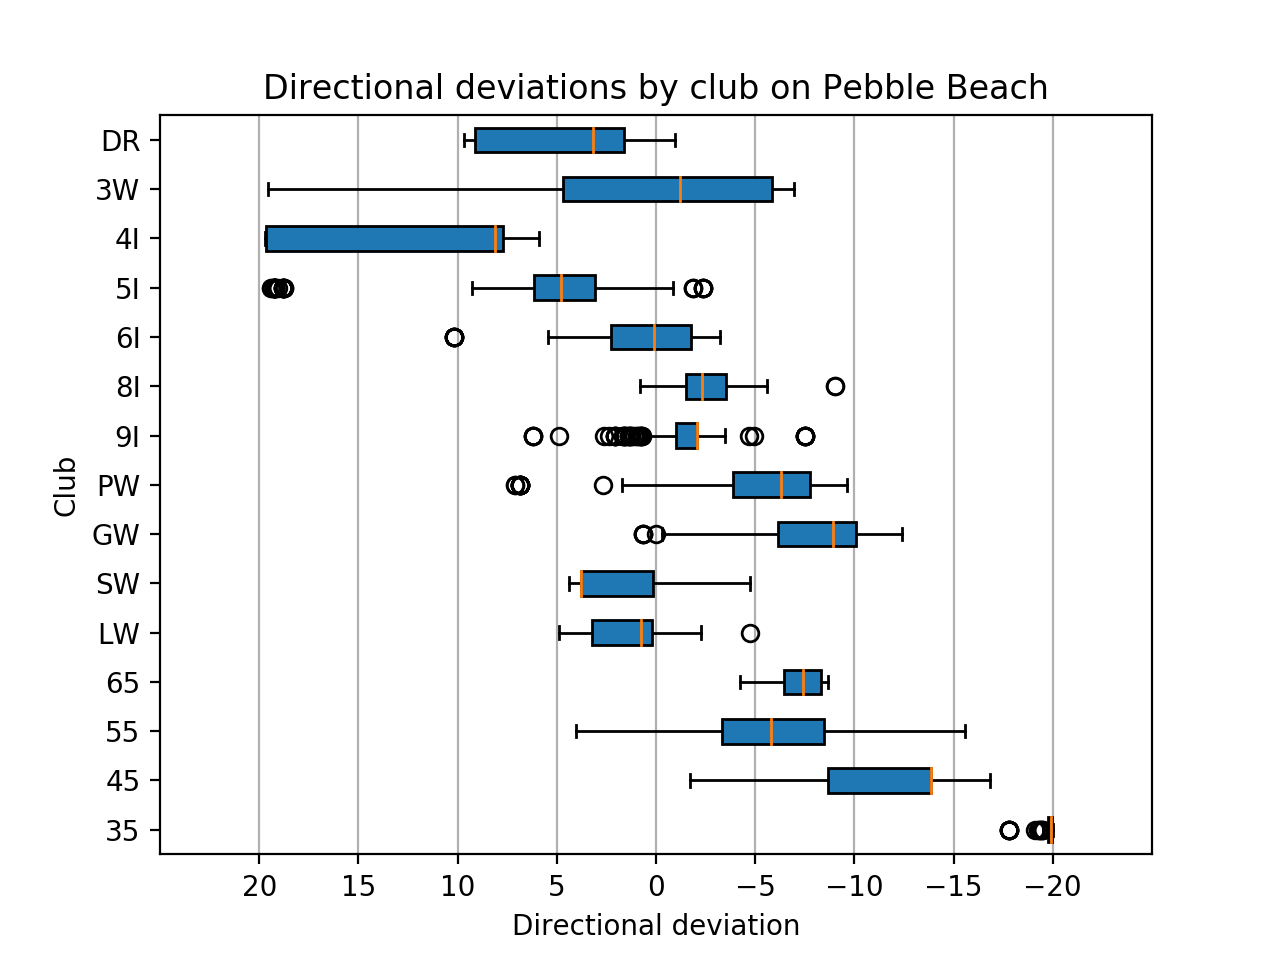
\includegraphics[width=0.5\textwidth]{Boxplots/MPDQN_Pebble_directions.png}
    \caption{Boxplots showcasing the directional deviations for each club by the MP-DQN agent on Pebble Beach.}
    \label{fig:MPDQN_pebble_direction_choices}
\end{figure}

\subsubsection{Ullna GC}
In \autoref{tab:ullna_average_results}, the average scores, number of shots and distances remaining for each hole on Ullna GC are presented for the golfer, the Dueling DDQN agent and the MP-DQN agent, respectively. Similarly to previously mentioned results, some holes were harder or easier than others for both the agents and the golfer. 

\begin{table}
    \begin{subtable}{\textwidth}
    \centering
    \begin{tabular}{c|c|c|c|c}
    \multicolumn{5}{c}{\textbf{Ullna GC Average Golfer Results}} \\
        \textbf{Hole} & \textbf{Par} & \textbf{Score} & \textbf{Shots} & \textbf{Distance remaining (m)}  \\ \hline
        1 & 5 & 0.32 & 2.75 & 13.75 \\ 
        2 & 4 & 0.27 & 2.00 & 12.50 \\ 
        3 & 3 & 0.17 & 1.00 & 9.65 \\ 
        4 & 5 & 0.40 & 3.25 & 23.25 \\ 
        5 & 3 & 0.37 & 2.50 & 14.85 \\ 
        6 & 4 & 0.25 & 2.00 & 6.67 \\ 
        7 & 4 & 0.32 & 2.25 & 18.00 \\ 
        8 & 4 & 0.28 & 2.00 & 15.75 \\ 
        9 & 4 & 0.28 & 2.00 & 14.50 \\ 
    \end{tabular}
    \end{subtable}
    \hfill
    \begin{subtable}{\textwidth}
    \centering
    \begin{tabular}{c|c|c|c|c}
    \multicolumn{5}{c}{\textbf{Ullna GC Average Dueling DDQN Results}} \\
        \textbf{Hole} & \textbf{Par} & \textbf{Score} & \textbf{Shots} & \textbf{Distance remaining (m)}  \\ \hline
        1 & 5 & 0.33 & 2.85 & 14.36 \\ 
        2 & 4 & 0.28 & 2.08 & 12.85 \\ 
        3 & 3 & 0.21 & 1.16 & 15.73 \\ 
        4 & 5 & 0.41 & 3.68 & 20.89 \\ 
        5 & 3 & 0.23 & 1.35 & 15.10 \\ 
        6 & 4 & 0.30 & 2.24 & 13.41 \\ 
        7 & 4 & 0.28 & 2.05 & 13.16 \\ 
        8 & 4 & 0.29 & 2.12 & 13.51 \\ 
        9 & 4 & 0.29 & 2.19 & 13.95 \\ 
    \end{tabular}
    \end{subtable}
    \hfill
    \begin{subtable}{\textwidth}
    \centering
    \begin{tabular}{c|c|c|c|c}
    \multicolumn{5}{c}{\textbf{Ullna GC Average MP-DQN Results}} \\
        \textbf{Hole} & \textbf{Par} & \textbf{Score} & \textbf{Shots} & \textbf{Distance remaining (m)}  \\ \hline
        1 & 5 & 0.34 & 2.96 & 14.14 \\ 
        2 & 4 & 0.30 & 2.26 & 12.11 \\ 
        3 & 3 & 0.19 & 1.08 & 14.32 \\ 
        4 & 5 & 0.35 & 3.02 & 16.23 \\ 
        5 & 3 & 0.25 & 1.55 & 13.67 \\ 
        6 & 4 & 0.33 & 2.42 & 15.46 \\ 
        7 & 4 & 0.29 & 2.18 & 13.85 \\ 
        8 & 4 & 0.30 & 2.21 & 15.79 \\ 
        9 & 4 & 0.29 & 2.18 & 13.80 \\ 
    \end{tabular}
    \end{subtable}
    \caption{The average scores, number of shots and distances remaining gathered from the golfer, Dueling DDQN agent and MP-DQN agent for each hole on Ullna GC, respectively. All numbers are rounded to two decimals.}
    \label{tab:ullna_average_results}
\end{table}

When looking at the average scores over all holes, both the Dueling DDQN agent and the MP-DQN agent performed better than the golfer. Just like with the Pebble Beach data, paired t-tests were conducted to determine the significance of the results. For the Dueling DDQN agent, all attributes were non-significant with $P = 0.865 > 0.05$, $P = 0.983 > 0.05$ and $P = 0.733 > 0.05$ for the scores, number of shots and distances remaining, respectively. The same was true for the MP-DQN agent, with $P = 0.991 > 0.05$, $P = 0.933 > 0.05$ and $P = 0.975 > 0.05$ for the scores, number of shots and distances remaining, respectively.

For more specific results regarding the scores of the golfer and the agents on Ullna GC, see \autoref{app:ullna_histograms}. This appendix showcases histograms that describes how often a score was achieved, a certain number of shots were hit, and a specific distance was remaining for the agents and the golfer.

In \autoref{app:ullna_club_choices}, the percentages of clubs chosen for the first, second and third shot on a given hole at Ullna GC are presented for the golfer and the Dueling DDQN and MP-DQN agents, respectively. Just like with the choices on Pebble Beach, both agents, as well as the golfer, trend rightwards in club selection from their first shots to their third shots. The only exception is the matrix for the third shot by the golfer, which contains only a few entries. This is because on Ullna GC, most holes the golfer played did not require a third shot before completion. Just like with the Pebble Beach matrices, there is a difference between the Dueling DDQN agent and MP-DQN agent, with the MP-DQN agent being more prone to hitting the DR.

In \autoref{fig:MPDQN_ullna_direction_choices}, the average directional choices made by the MP-DQN agent for each club are shown. As is shown in the table, the agent deviated on average well within the limits for all clubs, unlike the agent trained on Pebble Beach. However, the signs of the directional deviations are flipped less often than the Pebble Beach agent's deviations, compared to the golfer's data in \autoref{fig:shot_data_angle}. That is, the deviations do not counter the average miss of the golfer's data as often.

\begin{figure}
    \centering
    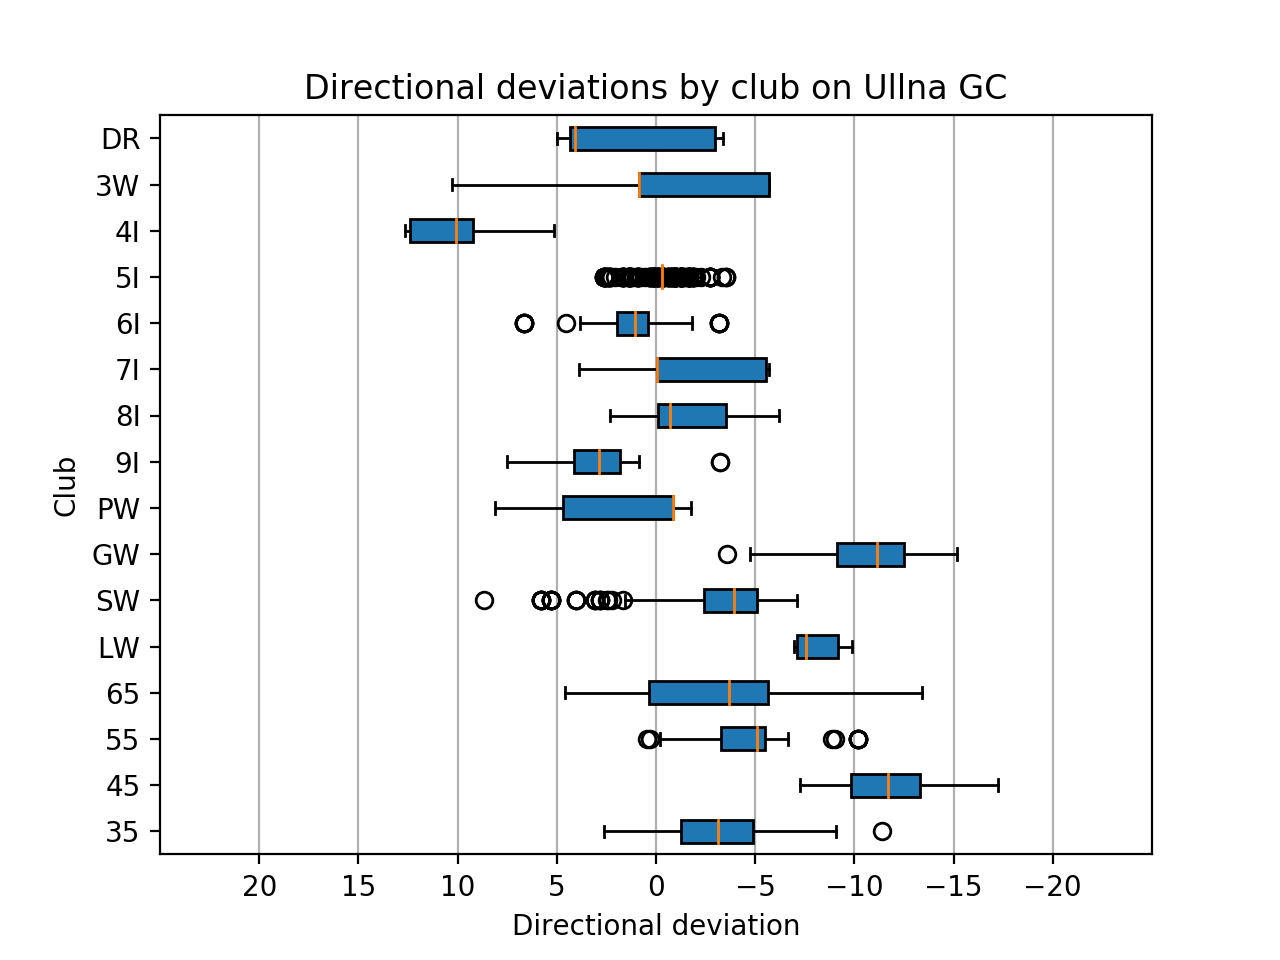
\includegraphics[width=0.5\textwidth]{Boxplots/MPDQN_Ullna_directions.png}
    \caption{Boxplots showcasing the directional deviations for each club by the MP-DQN agent on Ullna GC.}
    \label{fig:MPDQN_ullna_direction_choices}
\end{figure}

\section{Summary}
To summarize this chapter; the golfer produced shot data that covered most distances between the shortest and longest shot and that in general did not contain large systematic misses left or right. The agents used this data during training and it was clear that they did learn during the training process. Specifically, both agents played on a similar level to the golfer on both Pebble Beach and Ullna GC, with only the distances remaining for the MP-DQN agent being significantly worse than the golfer on Pebble Beach. Furthermore, club choices and similar attributes were retrieved from the agents, showing some similarities with the golfer but also some differences. These attributes will be used in the following chapter to discuss the performance of the agents.

\chapter{Discussion}
\label{chapter:discussion}
In this chapter, the results presented in \autoref{chapter:results} are analyzed and discussed. The reasons behind the results are examined, and other interesting points from this thesis are brought up. Finally, the limitations on the results are presented and potential future research is talked about.

\section{Analysis of the Results}
It is clear from the results and significance tests that both agents played neither better nor worse than the golfer. All tests were non-significant, aside from the MP-DQN agent trained on Pebble Beach being worse in regards to distance remaining. In regards to the research question of this thesis, how well reinforcement learning agents compare to a golfer when playing golf using the golfer's shot data, it is therefore possible to say that the agents can play at least on a similar level to the golfer.

It is interesting to discuss why this is the case, i.e. the reasons behind the agents being able to play on a similar level. One possible reason is that the problem of playing golf fits well with reinforcement learning agents. Even though there are many state and action combinations, the scores propagate quickly through the agent networks due to an episode consisting of at most ten actions. For instance, a single action should be enough to determine the outcome of a par three hole, since in general only one shot is needed for those holes. This allows the agents to quickly learn what actions are good to take early on a hole, and these good actions in turn make it easier to figure out what actions are good to take later on a hole, resulting in a good score.

Given these results, it is also interesting to discuss why the agents did not perform better than the golfer. Due to their trial and error learning method, they should be able to figure out problems that the golfer has with their swing and learn how to counter them. There are several possible answers to this question. One is that the golfer already played optimally. If the golfer always chooses the correct club and direction to hit in, the agents could never become better but at most play as well as the golfer. It is however hard to determine if this was the case since no analysis has been done in regards to how well the golfer played the courses. It does seem unlikely, since the agents managed to play better than the golfer on some holes, for instance the fifth hole at Ullna GC. 

Another reason for the agents not outperforming the golfer could be that the data gathered from the golfer was non-representative of the golfer's actual performance. This could be either the shot data used by the agents or the course data used to compare the agents with the golfer. For instance, the golfer might have played especially well when gathering the course data, compared to when hitting shots for the agents to use. This might sound unlikely given that the data was collected at the same time and therefore should not be affected by potential surges in form, but there are two reasons why this could be the case. The first reason is the lack of data available from the golfer playing courses. Only five and four rounds were gathered from Pebble Beach and Ullna GC, respectively. This might have been too few rounds to accurately determine the performance of the golfer, and could have skewed the results in favor of the golfer.

The second reason for non-representative data could be that the way the data was gathered caused a performance difference between the course data and the shot data used by the agent. When gathering the shot data, the golfer only had a target direction to hit in, but no distance or specific target to aim for. Furthermore, aside from the distance clubs between 35 and 65 meters, all shot were full swings. These restrictions were not present when gathering the course data. The golfer was allowed to hit all kinds of shots when playing the holes. Moreover, the golfer also had specific targets to aim for, both in regards to distance and direction. Having specific targets may have made it easier to visualize and execute shots that were better suited given the current state of the golfer, and not always requiring full swings could have caused the golfer to adjust to distances where no club fit perfectly. As such, the course data might actually showcase a better performing golfer than the shot data used by the agents.

What these potential data deviations mean in terms of the results is most likely that the agents were compared with data that was not directly comparable, yet still performed similar to it. In that case, the agents might have been able to outperform the golfer with no way of showing that they did. It is however hard to determine if this is the case. Given that more experienced golfers most likely have more control over their swing and more knowledge in visualizing and executing shots depending on targets, it is likely that the potential difference between course data and shot data is smaller for a more inexperienced golfer. By gathering data from an inexperienced golfer, it would be possible to examine this further.

One other possible reason for the agents not playing better than the golfer is that the problem might be too complex. This may sound counterintuitive to the above statements of the problem fitting well with reinforcement learning, but it might be the case that the number of state and action combinations actually affect the results. The agents may know very well what to do in states that occur often, but have a worse knowledge of what to do when in states they rarely enter. Every shot counts a lot when playing golf, so one wrong action could significantly affect the results.  For instance, \autoref{fig:GW_shots} in \autoref{app:shot_data} showcases the shots hit with the GW, with one clear outlier compared to the rest of the shots. It is unlikely that the outlier is the sampled shot when choosing the GW club, but once it is sampled, the agent may end up in a state it can't infer much from, causing the score of the hole to worsen a lot compared to if any other GW shot had been hit.

The above mentioned potential problem is worsened when more shots are hit on a hole and where hazards are present, since the number of potential states grows exponentially for each club choice and when having to take into consideration where balls may be dropped. We can see that this is the case on one of the harder holes played, hole six on Pebble Beach. This is a long par five with several elevation changes and with the Pacific Ocean acting as a water hazard on the entirety of the right side of the hole. As can be seen in \autoref{tab:pebble_average_results} and in \autoref{app:pebble_histograms}, the Dueling DDQN agent is significantly affected by this. Furthermore, in \autoref{fig:DDDQN_pebble_club_choice_confusion} in \autoref{app:pebble_club_choices}, it is shown that this hole has one of the larger spreads in club selection over the first to third shot. This showcases the potential number of states the agent can end up in. The MP-DQN agent manages to handle this problem because it can aim left, making it possible to avoid the water hazard which in turn makes it possible to reduce the number of shots needed, but it is still affected and performs worse than the golfer. 

It is important to note that even though the agents did not perform better than the golfer when looking at the average results of the holes, they did in some cases actually play better. For instance, as is shown in \autoref{app:pebble_histograms}, more than 40\% of the time the agents only hit two shots on the par five second hole on Pebble Beach, whereas the golfer only did it 20\% of the time. The same is true for the par four seventh hole on Ullna GC, as shown in \autoref{app:ullna_histograms}, where the Dueling DDQN agent never performed worse than the golfer, but hit two shots over 90\% of the time compared to the golfer's 75\%. Similarly, the MP-DQN agent also hits two shots more often than the golfer, while being worse less than 5\% of the time. 

In general, the histograms showcase that the golfer is more consistent than the agents. That is, the golfer produces results that are more similar to each other, whereas the agents in a few cases produce results worse than the usual results. This is clear from \autoref{fig:pebble_shot_histograms} and \autoref{fig:ullna_shot_histograms}, where the agents for most holes have poor results in around 5\% to 10\% of the cases. It is possible that these results affect the performance of the agents enough for them to not perform better than the golfer. As was mentioned above, the complexity of the problem could have affected the agents' knowledge in states occurring later on the hole due to a lack of exploring in those states. As such, the agents could be causing these poor results because of this complexity. It could therefore be the case that allowing the agents to explore more would result in fewer outliers.

It should also be noted that the histograms for the golfer, as mentioned, might not accurately tell the performance of the golfer, due to the lack of data available. It could be the case that with more rounds gathered, less consistent results would be present for the golfer as well. 

The above mentioned example with the sixth hole at Pebble Beach clearly indicates why the Dueling DDQN agent might not have been able to outperform the golfer; the lack of directional input causes it to become incapable of avoiding hazards or obstacles. The target line is biased towards being in a good position, so if that is not the case, it might be impossible for the Dueling DDQN agent to escape the current bad state. It is therefore interesting that both the Dueling DDQN agent and the MP-DQN agent played similarly to the golfer. The MP-DQN agent should be able to perform better, like it does on Pebble Beach's sixth hole, but in general it does not. 

One possible reason for why the MP-DQN agent does not perform better than the Dueling DDQN agent is yet again the complexity of the problem. The selection of a directional deviation not only makes the action space more complex, but also the state space. With the Dueling DDQN agent, there are a finite number of states that the agent could end up in, dependent on the sampled shots and club choices. This number is huge when looking at the number of holes, number of shots possible on the holes and the number of shots available. However, when adding the directional deviation, a continuous interval, into the mix, the possible states that the agent can end up in becomes a continuous space instead. This might affect how well the agent is capable of learning, especially given the same time frame of 50000 episodes as the Dueling DDQN agent.

The learning graphs in \autoref{fig:training_plots} further showcase the added complexity when introducing direction. For the Dueling DDQN agent, the plots trend downwards from the start. The MP-DQN agent plots not only start at a higher score, but also trend upwards before the agents start learning information. This showcases that the MP-DQN agents need to explore more before actually learning something about the problem. It is therefore possible that a suboptimal solution is found due to the lack of extra training compared to the Dueling DDQN agent.

A clear example of where this added complexity could have affected the agent is through the MP-DQN agent's usage of the 35 on Pebble Beach. When looking in \autoref{fig:MPDQN_pebble_club_choice_confusion}, it is shown that the agent uses the 35 for many of its third shots. This most likely stems from good initial club choices, but sampling problems that caused it to end up just outside the finishing range of 30m. However, when looking at the directional deviations with the 35 on Pebble Beach in \autoref{fig:MPDQN_pebble_direction_choices}, it is shown that the agent aims almost as far right as it can for all shots. When looking at the shot data in \autoref{fig:35_shots} and \autoref{fig:shot_data_angle}, it is shown that the shots are not even close to needing that much of a directional deviation to end up close to the hole. Unless there are obstacles in the way, this is clearly a suboptimal choice, but the areas around the green are usually cleared from obstacles. This result could therefore stem from the lack of exploration performed by the agent in these types of states, due to them rarely occurring, with even more complexity of having to learn the direction as well. 

One example where the MP-DQN agent should outperform the Dueling DDQN agent is par three holes. In general, only one shot is needed to reach a terminal state on a par three. As such, both agents should quickly realize which club is the optimal choice on the hole. Furthermore, the MP-DQN agent should be able to determine the directional deviation required to get the ball close to the hole. However, when looking at the results in \autoref{tab:pebble_average_results} and \autoref{tab:ullna_average_results}, this is not clearly the case. Only on the third hole at Ullna GC does the MP-DQN agent improve in all regards compared to the Dueling DDQN agent. Moreover, when looking at the histograms in \autoref{app:pebble_histograms} it is shown that the MP-DQN agent has the worst distance distribution of all holes on the par three fifth hole on Pebble Beach. This is further added upon with the fact that the only significantly worse result was the distance remaining for the MP-DQN agent on Pebble Beach, and this was with a large effect size. 

One possible explanation to the above results is the definition of the scoring function. The distance remaining is never more important than the number of shots, and the MP-DQN agent could have learned to utilize its directional choices in terms of that. For instance, a water hazard on a hole can affect the number of shots due to penalty strokes incurred when hitting into it. The MP-DQN agent might therefore have come to the conclusion that it is smarter to deviate enough such that the hazards are not in play than deviate enough so that the distance remaining is minimized. This might in turn have come at the cost that the distance remaining is increased in order to make sure the number of shots is as low as possible. 

The above explanation is backed up by the results from the seventh hole on Pebble Beach. As is seen in \autoref{app:pebble_histograms}, the distance remaining is increased for the MP-DQN agent compared to the Dueling DDQN agent, but the number of shots needed is decreased. However, the opposite is true for the fifth hole on Ullna GC, as is shown in \autoref{app:ullna_histograms}. It could therefore be the case that these results also stem from the added complexity of the problem.

Finally, one possible reason for why the MP-DQN agent did not outperform the Dueling DDQN agent could be the fact that the shot data generally was straight. Most average offline angles were not large, as shown in \autoref{fig:shot_data_angle}. Since the Dueling DDQN always aims straight towards the target line, and the data generally was pretty straight, there might not have been much room for improvement for the MP-DQN agent. The difference could have been much larger with data with greater systematic misses in some direction.

Given the results when considering agents only trained and evaluated on one course, it is interesting to discuss how well the agents generalize to other courses. For instance, how well does an agent trained on one or more courses play on an unseen course, or how well does an agent trained on several courses play on a course it has been trained on? A few tests were actually performed to look into these questions, but were excluded from the thesis to keep it clean in regards to the research question. Instead, the findings are briefly discussed here.

The tests looked into how well an agent trained on three courses played on the unseen course Ullna GC as well as the seen course Pebble Beach. They also looked into how well the agent trained on Pebble Beach played on Ullna GC. On all courses evaluated, the agents played significantly worse than the golfer. This indicates that the agents used in this paper overfit to the courses trained on. However, it should be noted that the agents tested on novel courses were trained for 50000 episodes as well. This could have affected the results. For instance, the agent trained on multiple courses may not have had the time to learn features from all courses. It might therefore have been possible for the agent to improve its performance on Pebble Beach with more training. Thus, more research would be required to determine how well a reinforcement learning agent can learn how to play golf in general.

As a final discussion point, it is interesting to talk about the complexity of the variable hybrid action space. As has already been mentioned, most reinforcement learning papers have dealt with either discrete or continuous problems, and in most cases these have been static. That is, the available actions do not change depending on the state. It is therefore not inherently clear how to best approach more complex action spaces. This was the case when implementing the agents in this thesis. As mentioned in \autoref{chapter:methods}, the agents were punished when choosing the DR in an illegal state and sent back to that state again. Before this method was tested, a filtering technique and mapping technique were tested. The former simply made sure the advantage value of the DR was the lowest of all club choices when choosing an action, rendering it impossible to pick that club, and when exploring, the DR was removed from the possible choices. The latter remapped the DR to the 3W when chosen in an illegal state, due to the similarities between the two clubs. 

For both of these approaches, the agents actually performed worse than agents where the DR could be used for every shot and agents where the DR could never be used. This clearly indicated that the approaches caused the agents to learn suboptimal policies. It is hard to determine why this was the case, and no rigorous analysis was performed to figure out why. It could be that the techniques were not part of the learning process but simply acted as an extra layer of filtering. The agents could therefore not learn how the DR could be used, which caused a suboptimal choice to be made in its stead. Regardless of the reasons behind the performances of various approaches, this was an important lesson learned when working with complex action spaces.

\section{Societal and Ethical Aspects}
\label{sec:ethics}
Whenever research is conducted, it is necessary to ask what the impact of the research will be on society. Even though there are good intentions behind the work, ideas can be twisted into something malicious instead. This section therefore deals with how this thesis' research will impact the world.

As mentioned in \autoref{chapter:introduction}, the work in this thesis can be used to figure out how to use reinforcement learning to help golfers improve their game, which can make coaching more accessible to golfers. However, it may also act as a device that does too much for the golfer. For instance, if the technology presented in this paper is improved upon such that it is usable on a golf course, then a golfer could get assistance for almost every shot they hit. Is it then really the golfer that is playing? Some may consider the use of this technology as cheating, and this might in turn be detrimental to the game.

The above problem might happen, but when compared to other aspects of golf most likely will not impact the state of the game much. First of all, the governing bodies of golf would most likely set rules in place for when this type of technology could be used, such as banning it from competition play. This is in line with similar technologies that can assist golfers on the course, such as slope measuring tools. Secondly, golf is a sport where competition is mainly against oneself. During non-competition rounds the only person to cheat against is oneself, so the use of the technologies presented in this thesis would not affect others, but be a choice each golfer has to make. As a final remark, professional golfers utilize caddies during competition. These do not only carry the clubs of the golfer, but also figure out distances, and help golfers in their club and shot choices. If the professionals are allowed help, then it might not be unreasonable to allow amateurs the same help as well.

Another ethical aspect to this research is the problem of not exactly knowing how the agents work. This is a general problem with the use of neural networks, since the information found in the networks is not easily visualized such that humans can comprehend it. Because of this problem, it can be believed that the agents work as expected, without knowing about specific cases where the agents might act irrationally. In the case of the work presented in this thesis, the consequences might not be big; the agent will play a hole of golf suboptimally. However, if this research is expanded into other fields, the consequences may be more dire. For instance, what if robots learn how to perform surgical incisions using data from human surgeons? If there is not full knowledge about the agent, there is always a risk of it performing an incision that might cost the life of a patient. The implementations of this technology must therefore be rigorously tested before being put into production.

\section{Sustainability}
Just like it is important to consider this thesis' societal and ethical impact, it is also important to look into how the research is regarded in terms of sustainability. Even if a paper provides useful research, it might not be worth pursuing further if it is unsustainable.

There are a few negative use cases of the research in this paper in terms of environmental sustainability. If the agents are improved upon further such that they can be used to provide golfers with information on how to improve, this might turn into a commercial product. Given that the agent is limited by human data, each golfer needs an individual agent that has to be trained. This will require a lot of training time and as such a lot of computational resources. This can consume a large amount of energy, which might not be sustainable. 

Another example of a negative environmental impact is that the product might increase the amount of time people spend golfing. Getting insight on how to improve might motivate golfers to play more golf, which in turn requires golf facilities to maintain their courses more. This maintenance uses a lot of water, and an increase of golfers on the courses might also cause an increased water usage. Although the probability of this research significantly impacting water consumption is unlikely, it is still worth noting. 

An increased golfing demand does not necessarily imply negative environmental consequences. If the demand is high enough, new golf courses may be developed. In an industrialized world with fewer and fewer green spaces, golf courses can contribute a lot. Trees planted on the courses can reduce carbon emissions, and if developed and maintained correctly, the courses can also act as wildlife preserves. 

Finally, as has already been mentioned in \autoref{sec:ethics}, the research in this thesis may bridge the gap of available knowledge between professional golfers with caddies and amateurs. This can be perceived as increased social sustainability, in that all golfers can become more equal on the golf course. 

\section{Limitations}
In this section, the limitations of this thesis are presented and discussed. The reasons behind these limitations are mentioned, and how these limitations affected the results is described.

As has already been mentioned above, one possible contributor to the results is the lack of data available. This is true both in regards to the golfer the data was gathered from, but also the lack of data from other golfers. First of all, the number of rounds might have been too low to accurately portray how well the golfer played. The significance of the results could therefore be wrong, and the analysis of the results could be skewed. However, the analysis also touches upon other aspects, so it is not necessarily the case that the results are invalid.

The lack of data from other golfers also affected the analysis because it made it hard to determine how skill level affects the performance of the agents. As mentioned above, the agents might play better than more inexperienced golfers. There is however no way of testing this in this thesis due to the lack of data. 

Both these problems were caused due to the lack of time when gathering data. Each data gathering occasion took three hours to complete, and there was a cost to use the facility for gathering the data. It was therefore not feasible for the scope of this paper to gather more data.

The lack of time was also present in other parts of the thesis. Training the agents was very time consuming, which made it hard to test different approaches. 50000 episodes of training took around 14 hours to complete and since time was limited for this project, this resulted in only some configurations being tested. For instance, training the agents for a significantly longer time than 50000 episodes was not possible. Furthermore, there was no time to perform a rigorous parameter tuning, and instead estimates utilizing the literature available were used. Finally, the option to try different scoring functions, or even different algorithms, was severely limited because of this lack of time.

The effects of the lack of time could be that the agents got stuck in local optimums in terms of the scoring function. It could have been possible for the agents to perform better had they been able to train for a longer time, or train with different configurations. 

A final limitation is the golfer from which the data was gathered from. Given the time and accuracy needed for the gathering process, a colleague was used. To maintain the accuracy of the data, the gathering process was slow and could therefore not be performed using an unknown test subject. There is therefore a potential bias in the data from the golfer knowing the purpose of the various data gathering components. 

\section{Future Research}
In this section, future research related to that of this paper is discussed. Research directly related to the work in this paper is touched upon, and other similar topics are explored.

From the discussion about the results and limitations, it is clear that further research could be done within this specific topic if given more data to work with. More data from the same person would help clarify the agents' performance compared to the golfer's, and more data from other people would determine how well the agents play in general compared to humans. It is also clear that the results could be investigated further by looking at the training time. Future research could try using better hardware or longer training times to see how that affects the agents' performance, and if that could reduce the risk of finding a local optimum compared to a global one.

The discussions from the previous sections in this chapter also talked about how other methods could be used. It would be worthwhile to investigate how changing the weight of the distance remaining in the scoring function affects the results of the agents. Furthermore, it would be interesting to see if other factors could yield an even better result. For instance, one could investigate a scoring function that takes into account the terrain the ball ends up in when calculating the punishment, i.e. giving a worse score if the agent is in the rough compared to the fairway. 

Another interesting research topic would be to compare the reinforcement learning agents not only to the golfer, but to other types of agents too. For instance, a deterministic rule based agent could be interesting to implement. This type of agent has the benefit of not needing any training time. However, it would require more implementation time in order to figure out how to handle different states. The comparison is therefore interesting, since it provides a trade-off that might be viewed differently depending on the implementer.

As has been mentioned in this paper, one use case of the agents would be to act as helpers to the golfer they have used data from. However, this thesis only looked into the feasibility of using reinforcement learning to teach artificial agents to play golf, and no experiments were performed to see if the agents can help golfers improve their game. This would therefore be an interesting topic to research. However, more investigation into the feasibility of the agents, as mentioned above, is most likely needed since there was no significant performance difference found. 

Instead of looking into how the agents can help golfers, it could be researched if the agents are useful as opponents to the golfer. The agents trained in this paper managed to play on a similar level to the golfer and could therefore act as opponents when playing. It would be interesting to see if golfers would find these opponents reasonable to play against.

Finally, one can look at the general problem instead of the golf specific variant. In this thesis, a reinforcement learning approach was applied to a problem in which data was provided to the agents to limit and personalize them. This can be provided in many other contexts. For instance, other sports could be tested, such as baseball, bowling or cricket. This would require the agent to receive some representative data from the players and a definition of how to simulate the sport. Another example is robot workers replacing human tasks and utilizing data from humans to learn how these tasks can be executed. Similar conditions as with the sports would be needed here as well. Investigating how well reinforcement learning agents act in these types of environments would not only yield a better understanding of the problem and how it can be solved in general, but probably also give more insight about complex action and state spaces.

\chapter{Conclusions}
\label{chapter:conclusions}
In this thesis, reinforcement learning agents limited by human data have been trained and evaluated on playing golf in order to determine how well they play compared to the golfer whose data they have been limited on. This was done because of the potential use cases of reinforcement learning agents as tutors on how to improve, for both this and similar problems.

Specifically, a Dueling Double Deep Q Network agent and a Multi Pass Deep Q Network agent were implemented for the above mentioned purpose. These agents could play holes of golf by choosing clubs to hit. The latter of the two agents could also choose the direction to hit in. These actions sampled a shot gathered from a golfer with the chosen club, that was then input into a simulated golf environment. 

The agents were trained on 50000 holes on two courses, Pebble Beach and Ullna GC. These courses were also used for evaluation, and the results from the agents were compared to the golfer's performance on the courses. The results showcased no statistical significance between either agent and the golfer in terms of the score on each hole.

It was concluded that the results showed that reinforcement learning agents are at least able to perform on a similar level as a golfer. However, there were no indications that they could not be able to perform better, and several reasons as to why they did not were discussed. Two main components were the lack of data available and the lack of time during the scope of the thesis. The former made it difficult to determine the confidence of the golfer's results, which could have made the comparison between the agents and the golfer inaccurate. The latter made it difficult to test several approaches, and could also have affected the agents' performance due to them reaching local optimums in terms of the scoring function instead of global optimums. Another discussed factor was the complexity of the problem, which not only included a large state space but also a complex action space. This complexity could have affected the agents when reaching states they had not explored much, causing outlier results of poor quality. It could also explain why the directional agent did not perform better than the non-directional one.

The agents were able to play on a similar level as the golfer, even though they were limited on training time, even though the data available was limited and even though the problem was complex. By putting more research into this problem and investigating longer training times, better data and other scoring functions, it is possible to generalize the results of this thesis, potentially giving way to an agent capable of playing better than a golfer it has gotten data from. To conclude this thesis, it is therefore clear there is potential in using reinforcement learning to play golf with an agent limited by human data.

\printbibliography[heading=bibintoc]

\appendix

\chapter{Shot Data}
\label{app:shot_data}
\begin{figure}
    \centering
    \begin{subfigure}{0.4\textwidth}
    \centering
    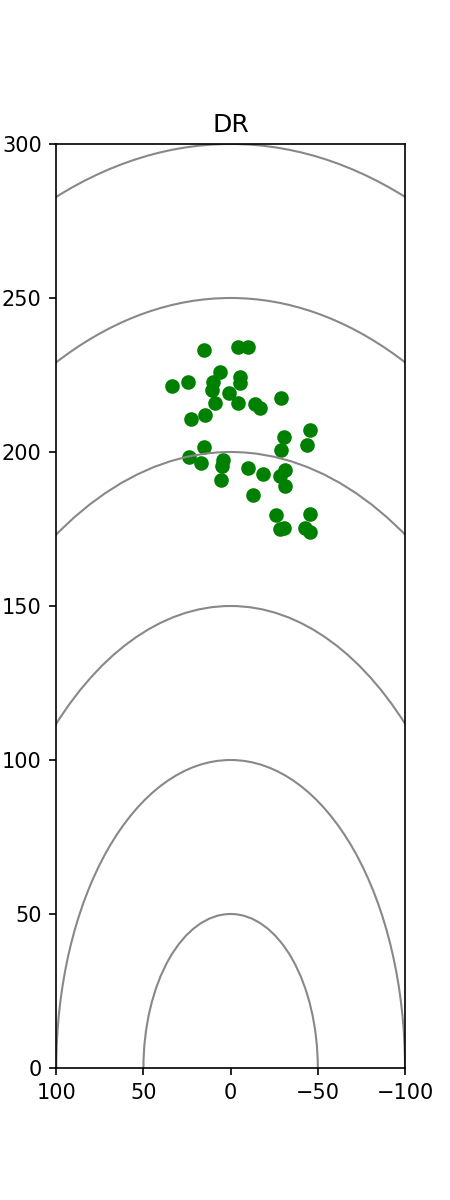
\includegraphics[height=0.4\textheight]{Shots/DR_shots.png} 
    \caption{The landing positions of the DR shots hit by the golfer.}
    \label{fig:DR_shots}
    \end{subfigure}
    \begin{subfigure}{0.4\textwidth}
    \centering
    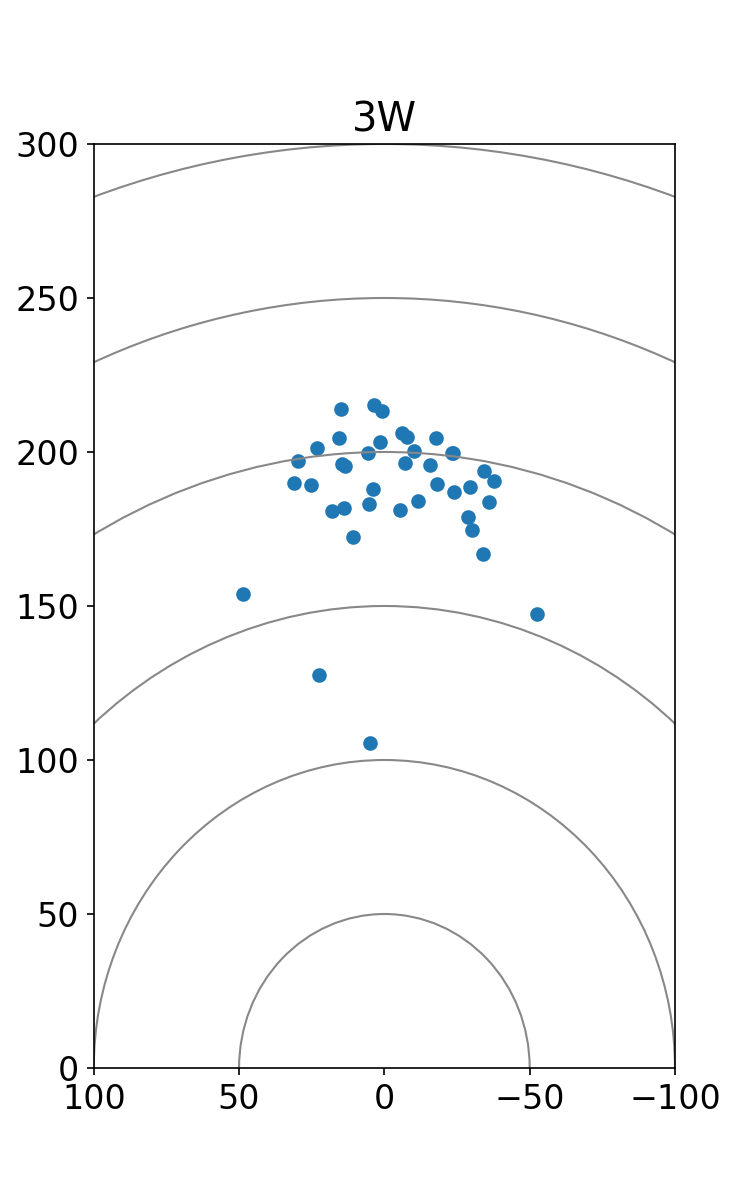
\includegraphics[height=0.4\textheight]{Shots/3W_shots.png} 
    \caption{The landing positions of the 3W shots hit by the golfer.}
    \label{fig:3W_shots}
    \end{subfigure}
    \begin{subfigure}{0.4\textwidth}
    \centering
    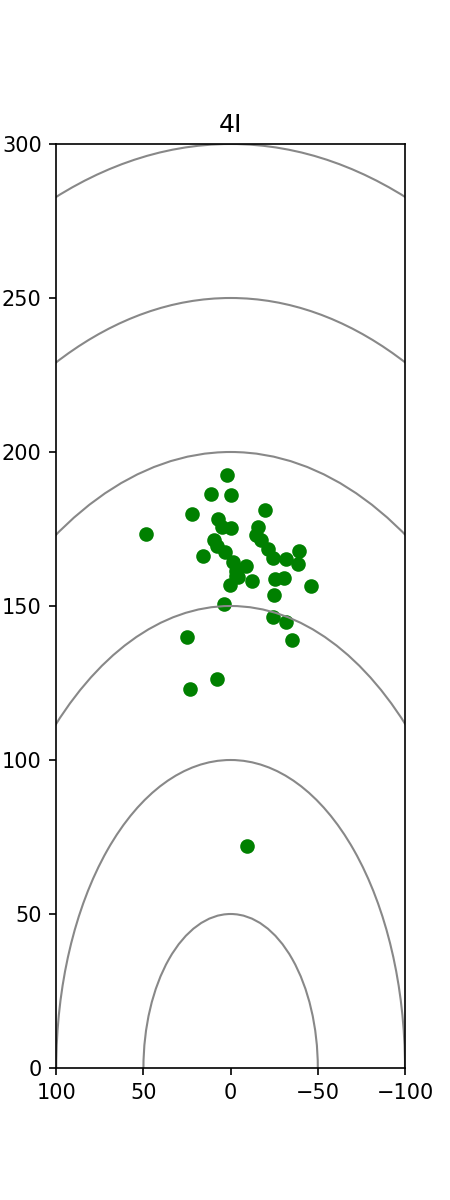
\includegraphics[height=0.4\textheight]{Shots/4I_shots.png} 
    \caption{The landing positions of the 4I shots hit by the golfer.}
    \label{fig:4I_shots}
    \end{subfigure}
    \begin{subfigure}{0.4\textwidth}
    \centering
    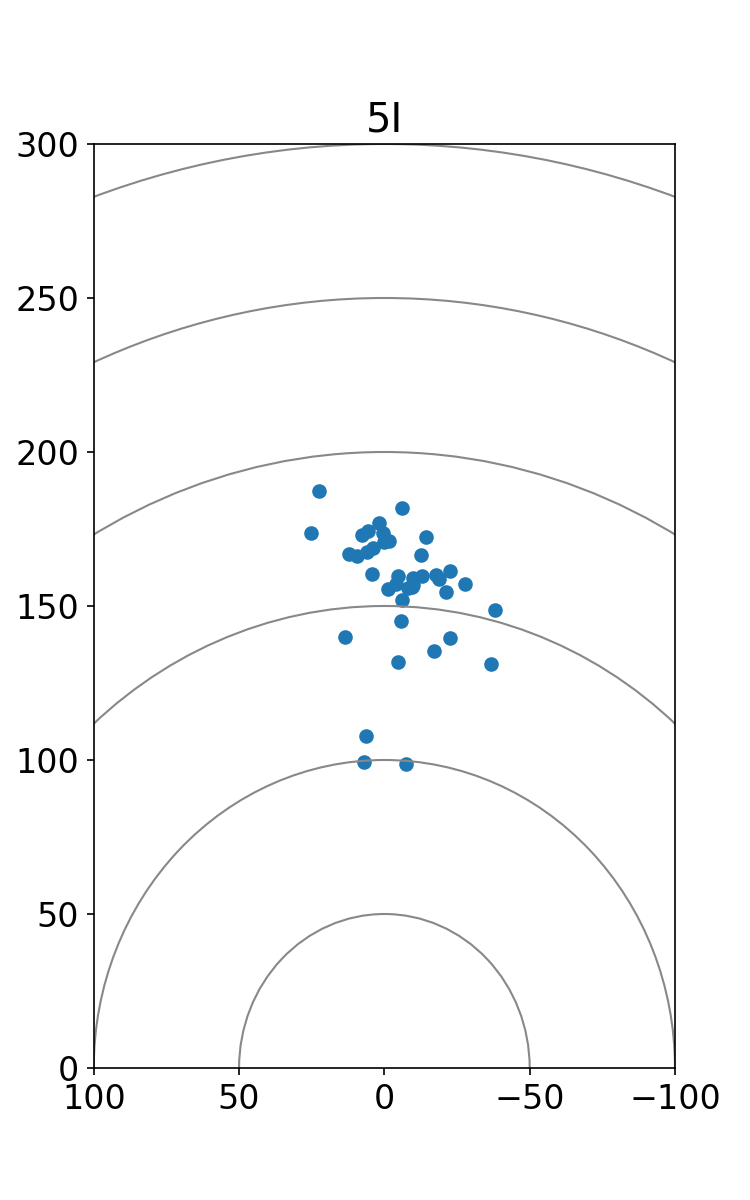
\includegraphics[height=0.4\textheight]{Shots/5I_shots.png} 
    \caption{The landing positions of the 5I shots hit by the golfer.}
    \label{fig:5I_shots}
    \end{subfigure}
\end{figure}

\begin{figure}
    \centering
    \begin{subfigure}{0.4\textwidth}
    \centering
    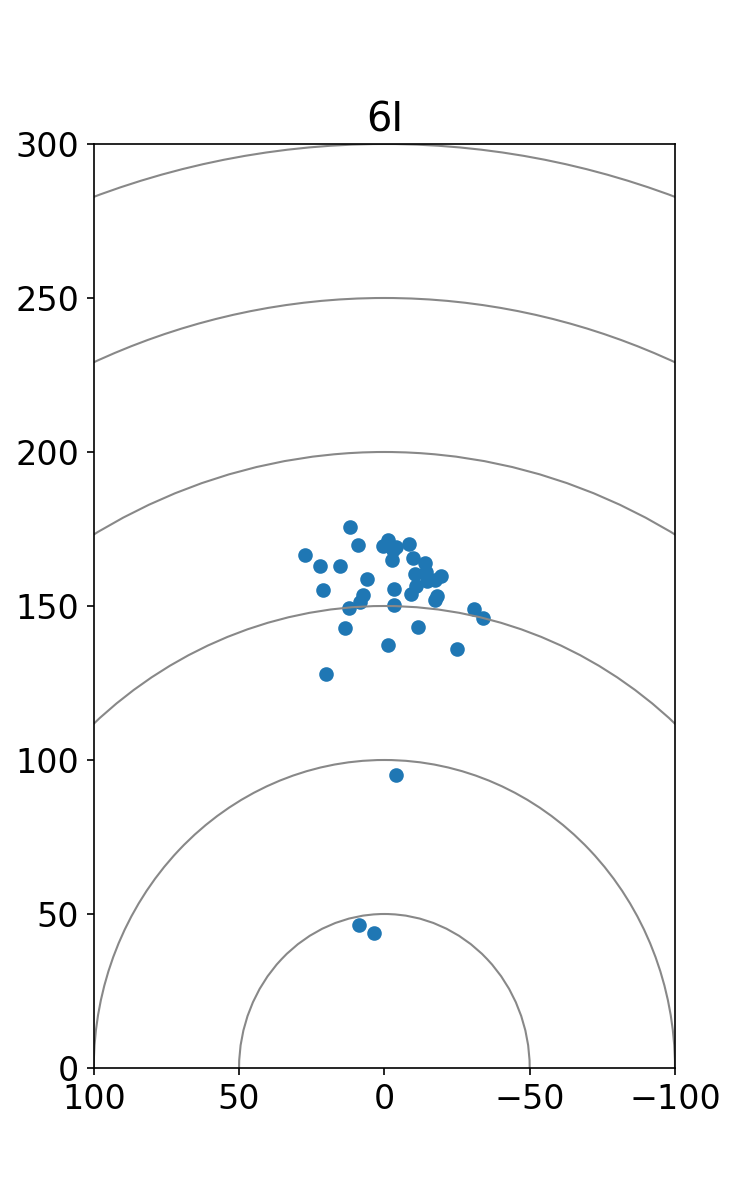
\includegraphics[height=0.4\textheight]{Shots/6I_shots.png} 
    \caption{The landing positions of the 6I shots hit by the golfer.}
    \label{fig:6I_shots}
    \end{subfigure}
    \begin{subfigure}{0.4\textwidth}
    \centering
    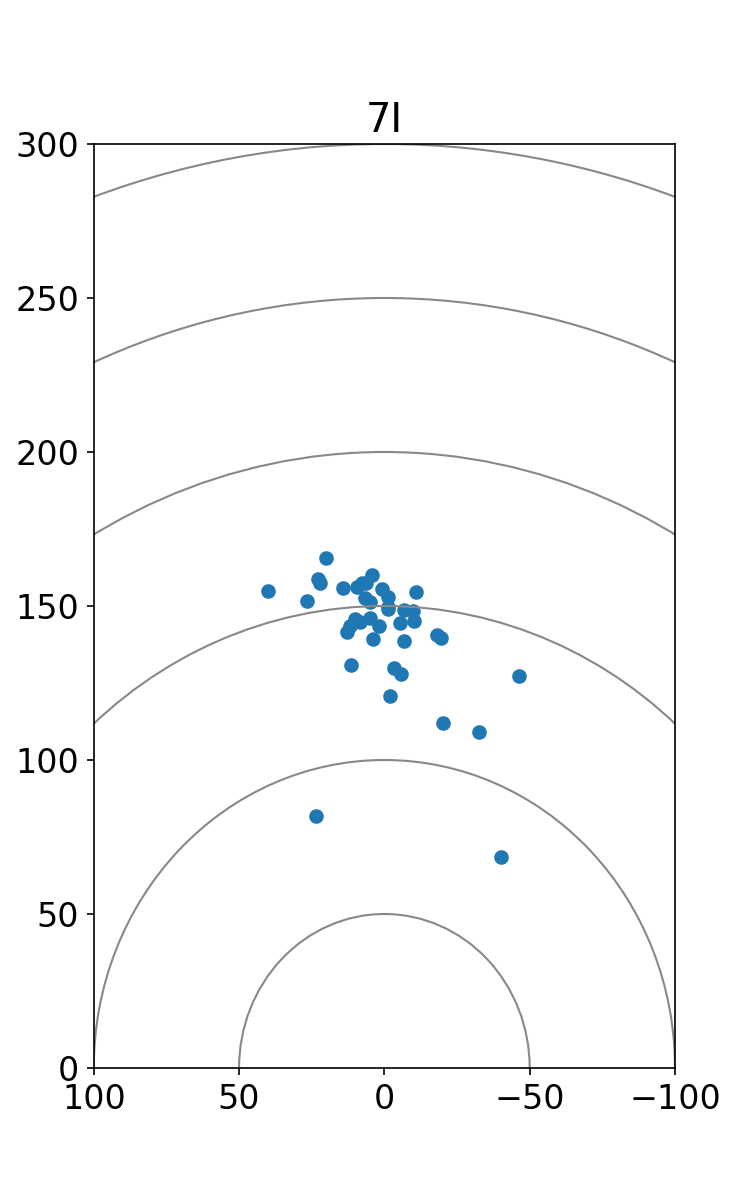
\includegraphics[height=0.4\textheight]{Shots/7I_shots.png} 
    \caption{The landing positions of the 7I shots hit by the golfer.}
    \label{fig:7I_shots}
    \end{subfigure}
    \begin{subfigure}{0.4\textwidth}
    \centering
    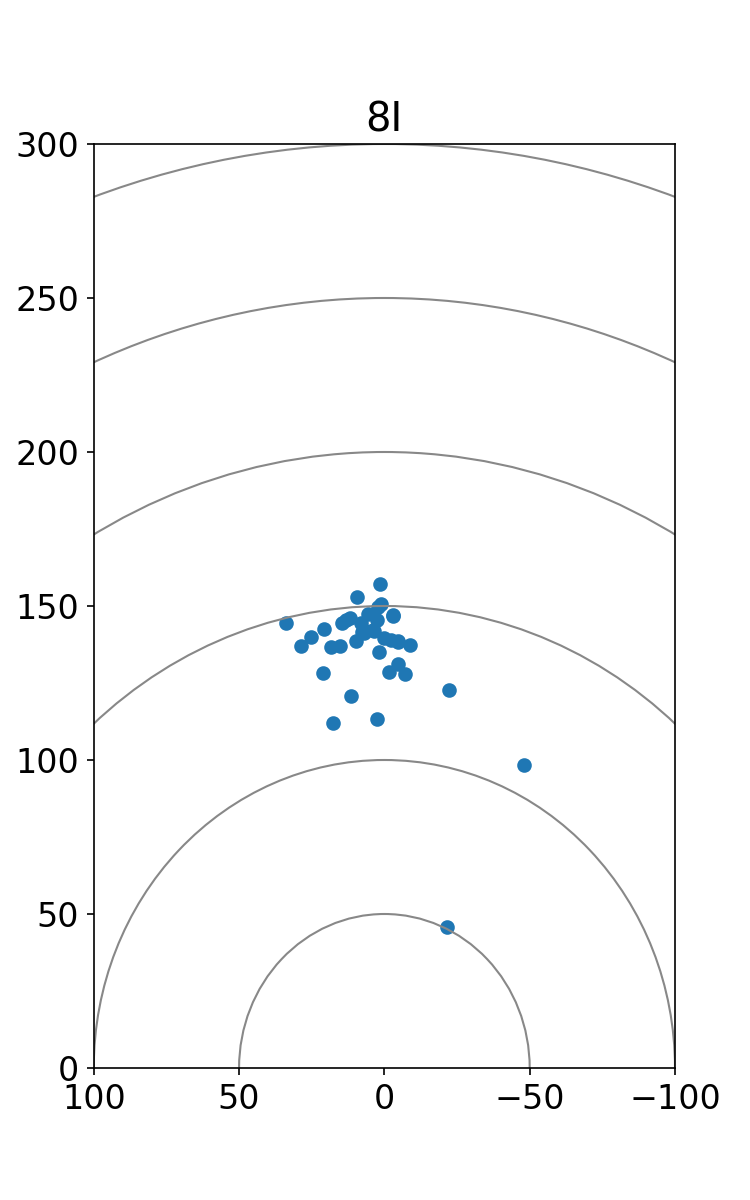
\includegraphics[height=0.4\textheight]{Shots/8I_shots.png} 
    \caption{The landing positions of the 8I shots hit by the golfer.}
    \label{fig:8I_shots}
    \end{subfigure}
    \begin{subfigure}{0.4\textwidth}
    \centering
    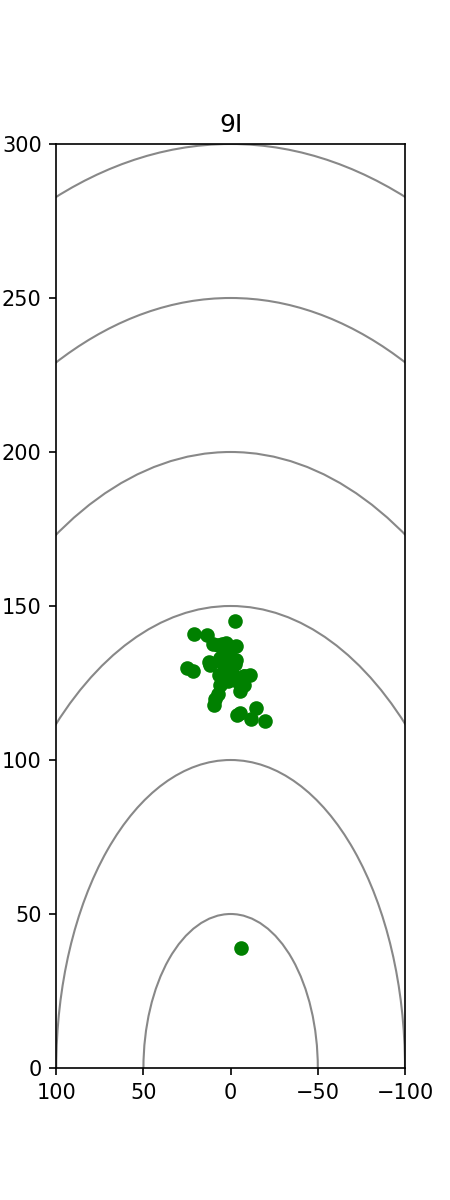
\includegraphics[height=0.4\textheight]{Shots/9I_shots.png} 
    \caption{The landing positions of the 9I shots hit by the golfer.}
    \label{fig:9I_shots}
    \end{subfigure}
\end{figure}

\begin{figure}
    \centering
    \begin{subfigure}{0.4\textwidth}
    \centering
    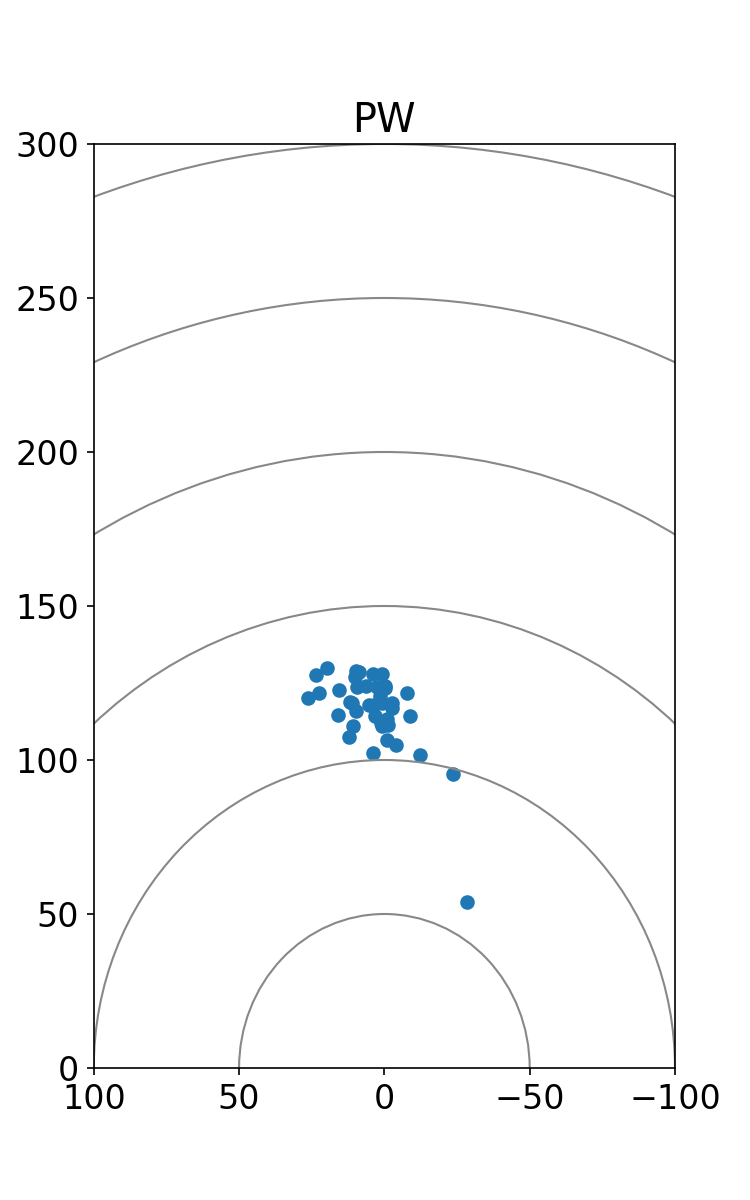
\includegraphics[height=0.4\textheight]{Shots/PW_shots.png} 
    \caption{The landing positions of the PW shots hit by the golfer.}
    \label{fig:PW_shots}
    \end{subfigure}
    \begin{subfigure}{0.4\textwidth}
    \centering
    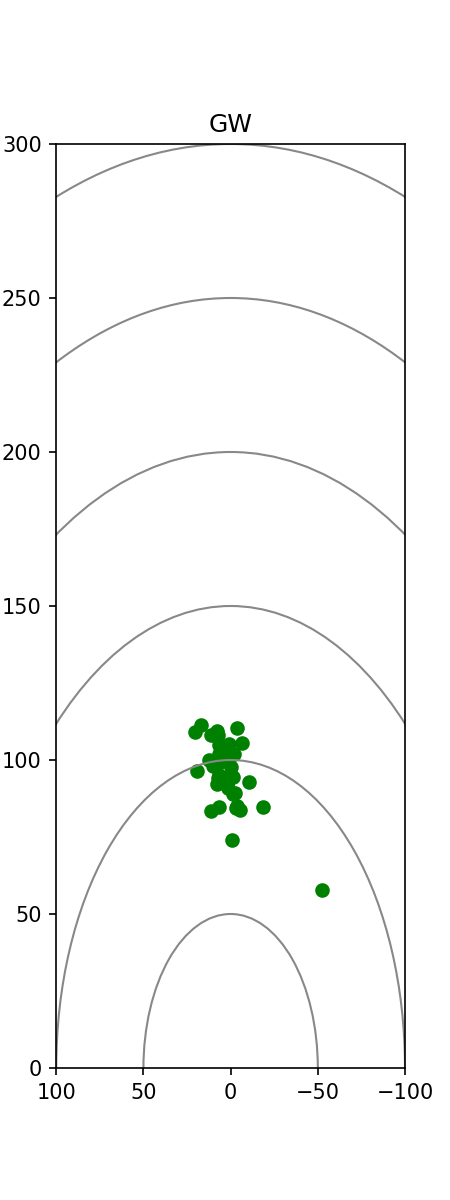
\includegraphics[height=0.4\textheight]{Shots/GW_shots.png} 
    \caption{The landing positions of the GW shots hit by the golfer.}
    \label{fig:GW_shots}
    \end{subfigure}
    \begin{subfigure}{0.4\textwidth}
    \centering
    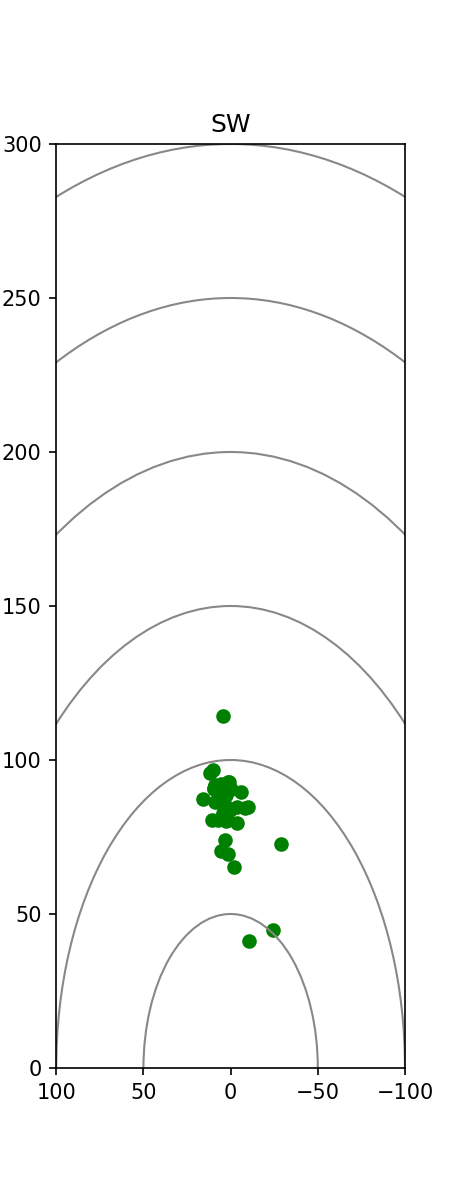
\includegraphics[height=0.4\textheight]{Shots/SW_shots.png} 
    \caption{The landing positions of the SW shots hit by the golfer.}
    \label{fig:SW_shots}
    \end{subfigure}
    \begin{subfigure}{0.4\textwidth}
    \centering
    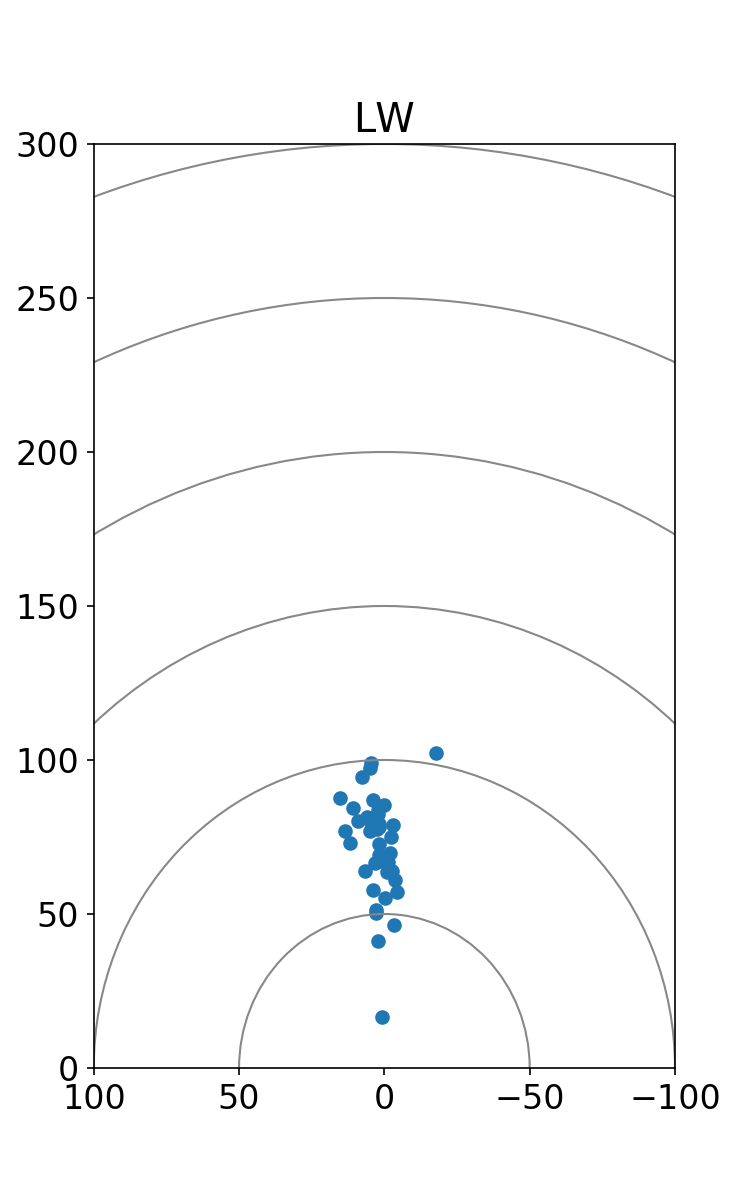
\includegraphics[height=0.4\textheight]{Shots/LW_shots.png} 
    \caption{The landing positions of the LW shots hit by the golfer.}
    \label{fig:LW_shots}
    \end{subfigure}
\end{figure}

\begin{figure}
    \centering
    \begin{subfigure}{0.4\textwidth}
    \centering
    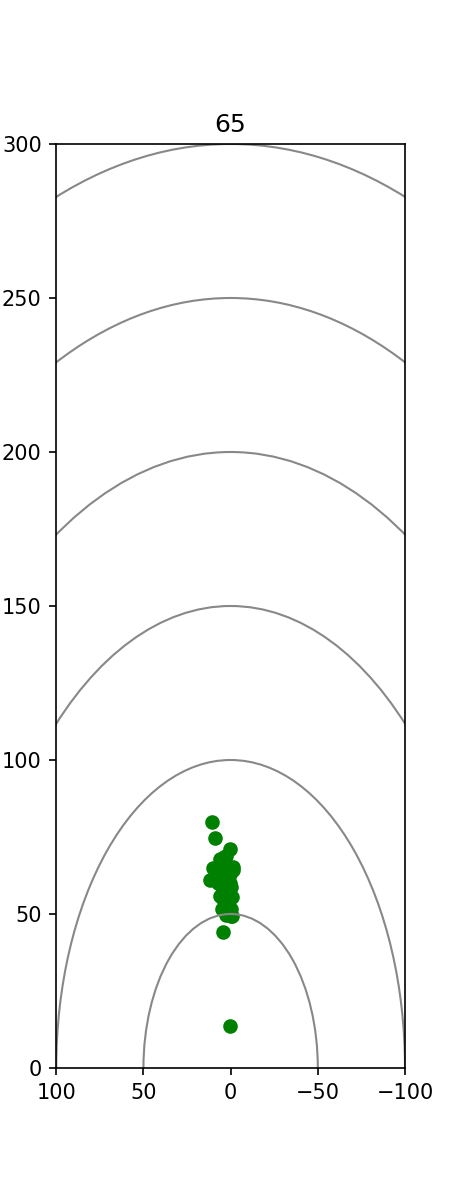
\includegraphics[height=0.4\textheight]{Shots/65_shots.png} 
    \caption{The landing positions of the 65 shots hit by the golfer.}
    \label{fig:65_shots}
    \end{subfigure}
    \begin{subfigure}{0.4\textwidth}
    \centering
    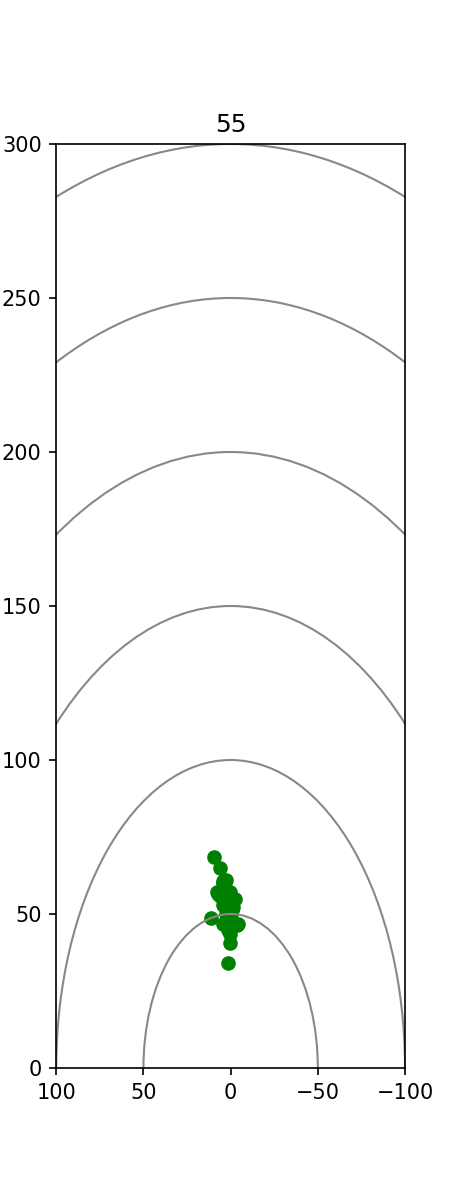
\includegraphics[height=0.4\textheight]{Shots/55_shots.png} 
    \caption{The landing positions of the 55 shots hit by the golfer.}
    \label{fig:55_shots}
    \end{subfigure}
    \begin{subfigure}{0.4\textwidth}
    \centering
    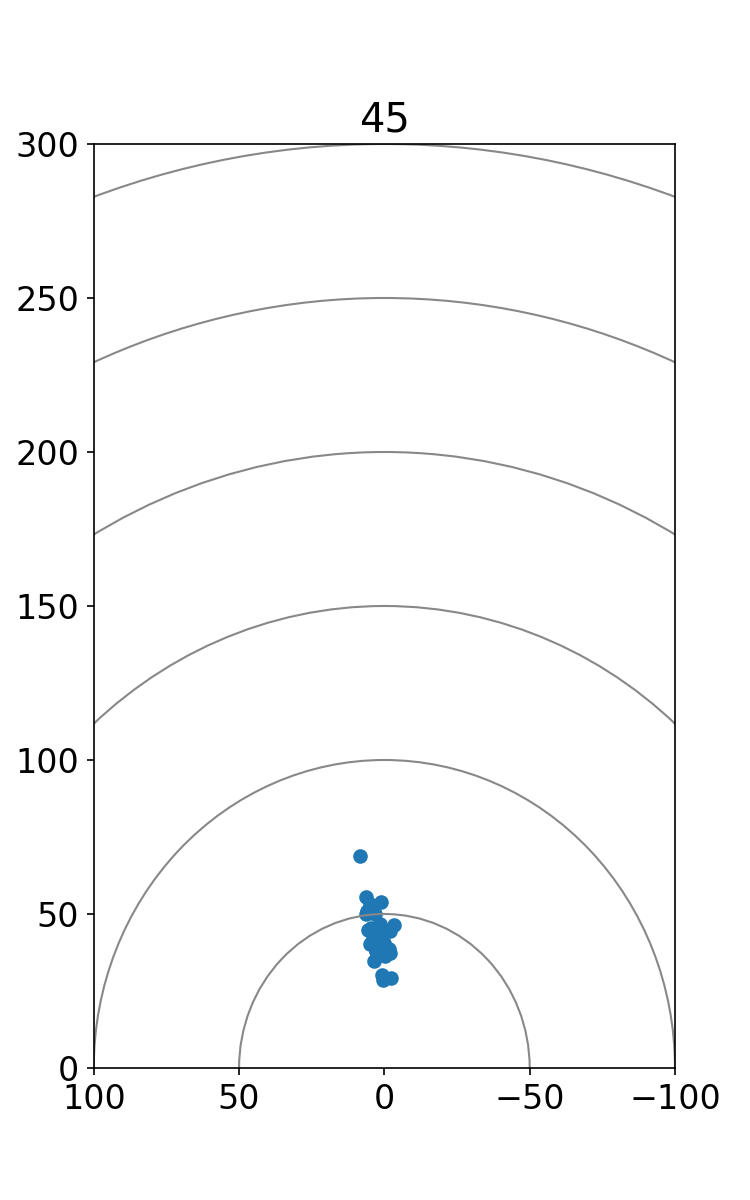
\includegraphics[height=0.4\textheight]{Shots/45_shots.png} 
    \caption{The landing positions of the 45 shots hit by the golfer.}
    \label{fig:45_shots}
    \end{subfigure}
    \begin{subfigure}{0.4\textwidth}
    \centering
    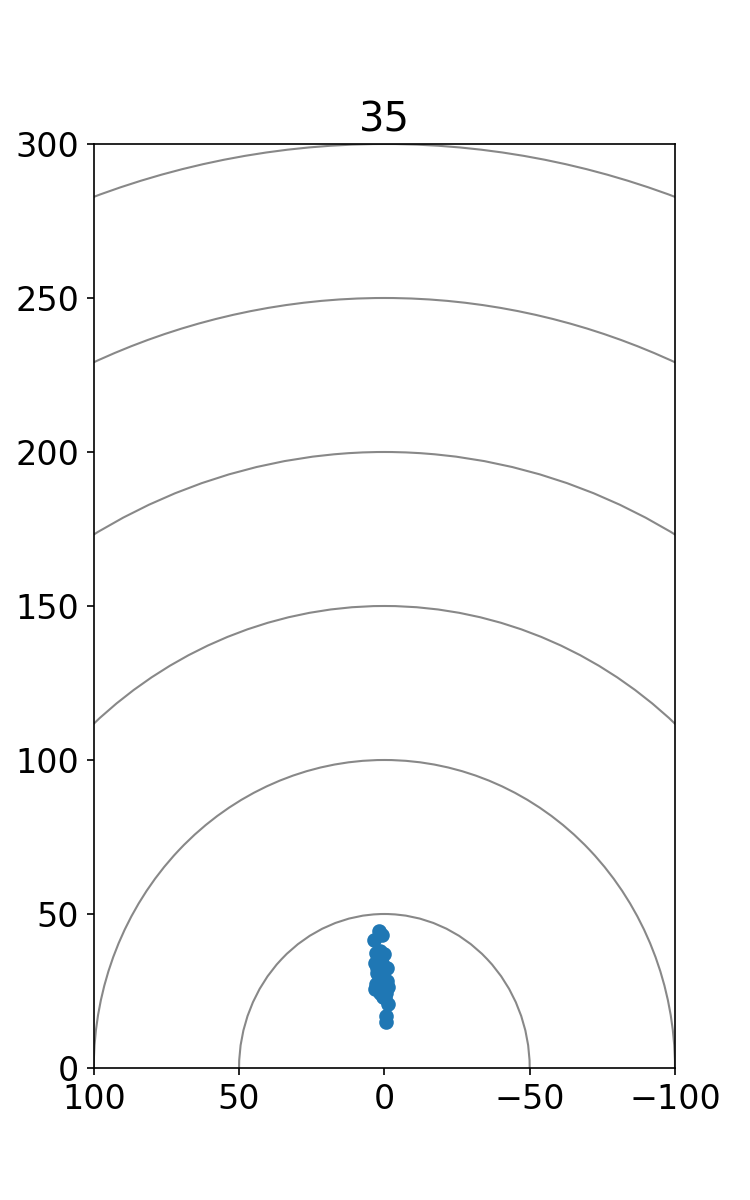
\includegraphics[height=0.4\textheight]{Shots/35_shots.png} 
    \caption{The landing positions of the 35 shots hit by the golfer.}
    \label{fig:35_shots}
    \end{subfigure}
\end{figure}

\chapter{Pebble Beach Histograms}
\label{app:pebble_histograms}
\begin{figure}
    \centering
    \begin{subfigure}{\textwidth}
    \centering
    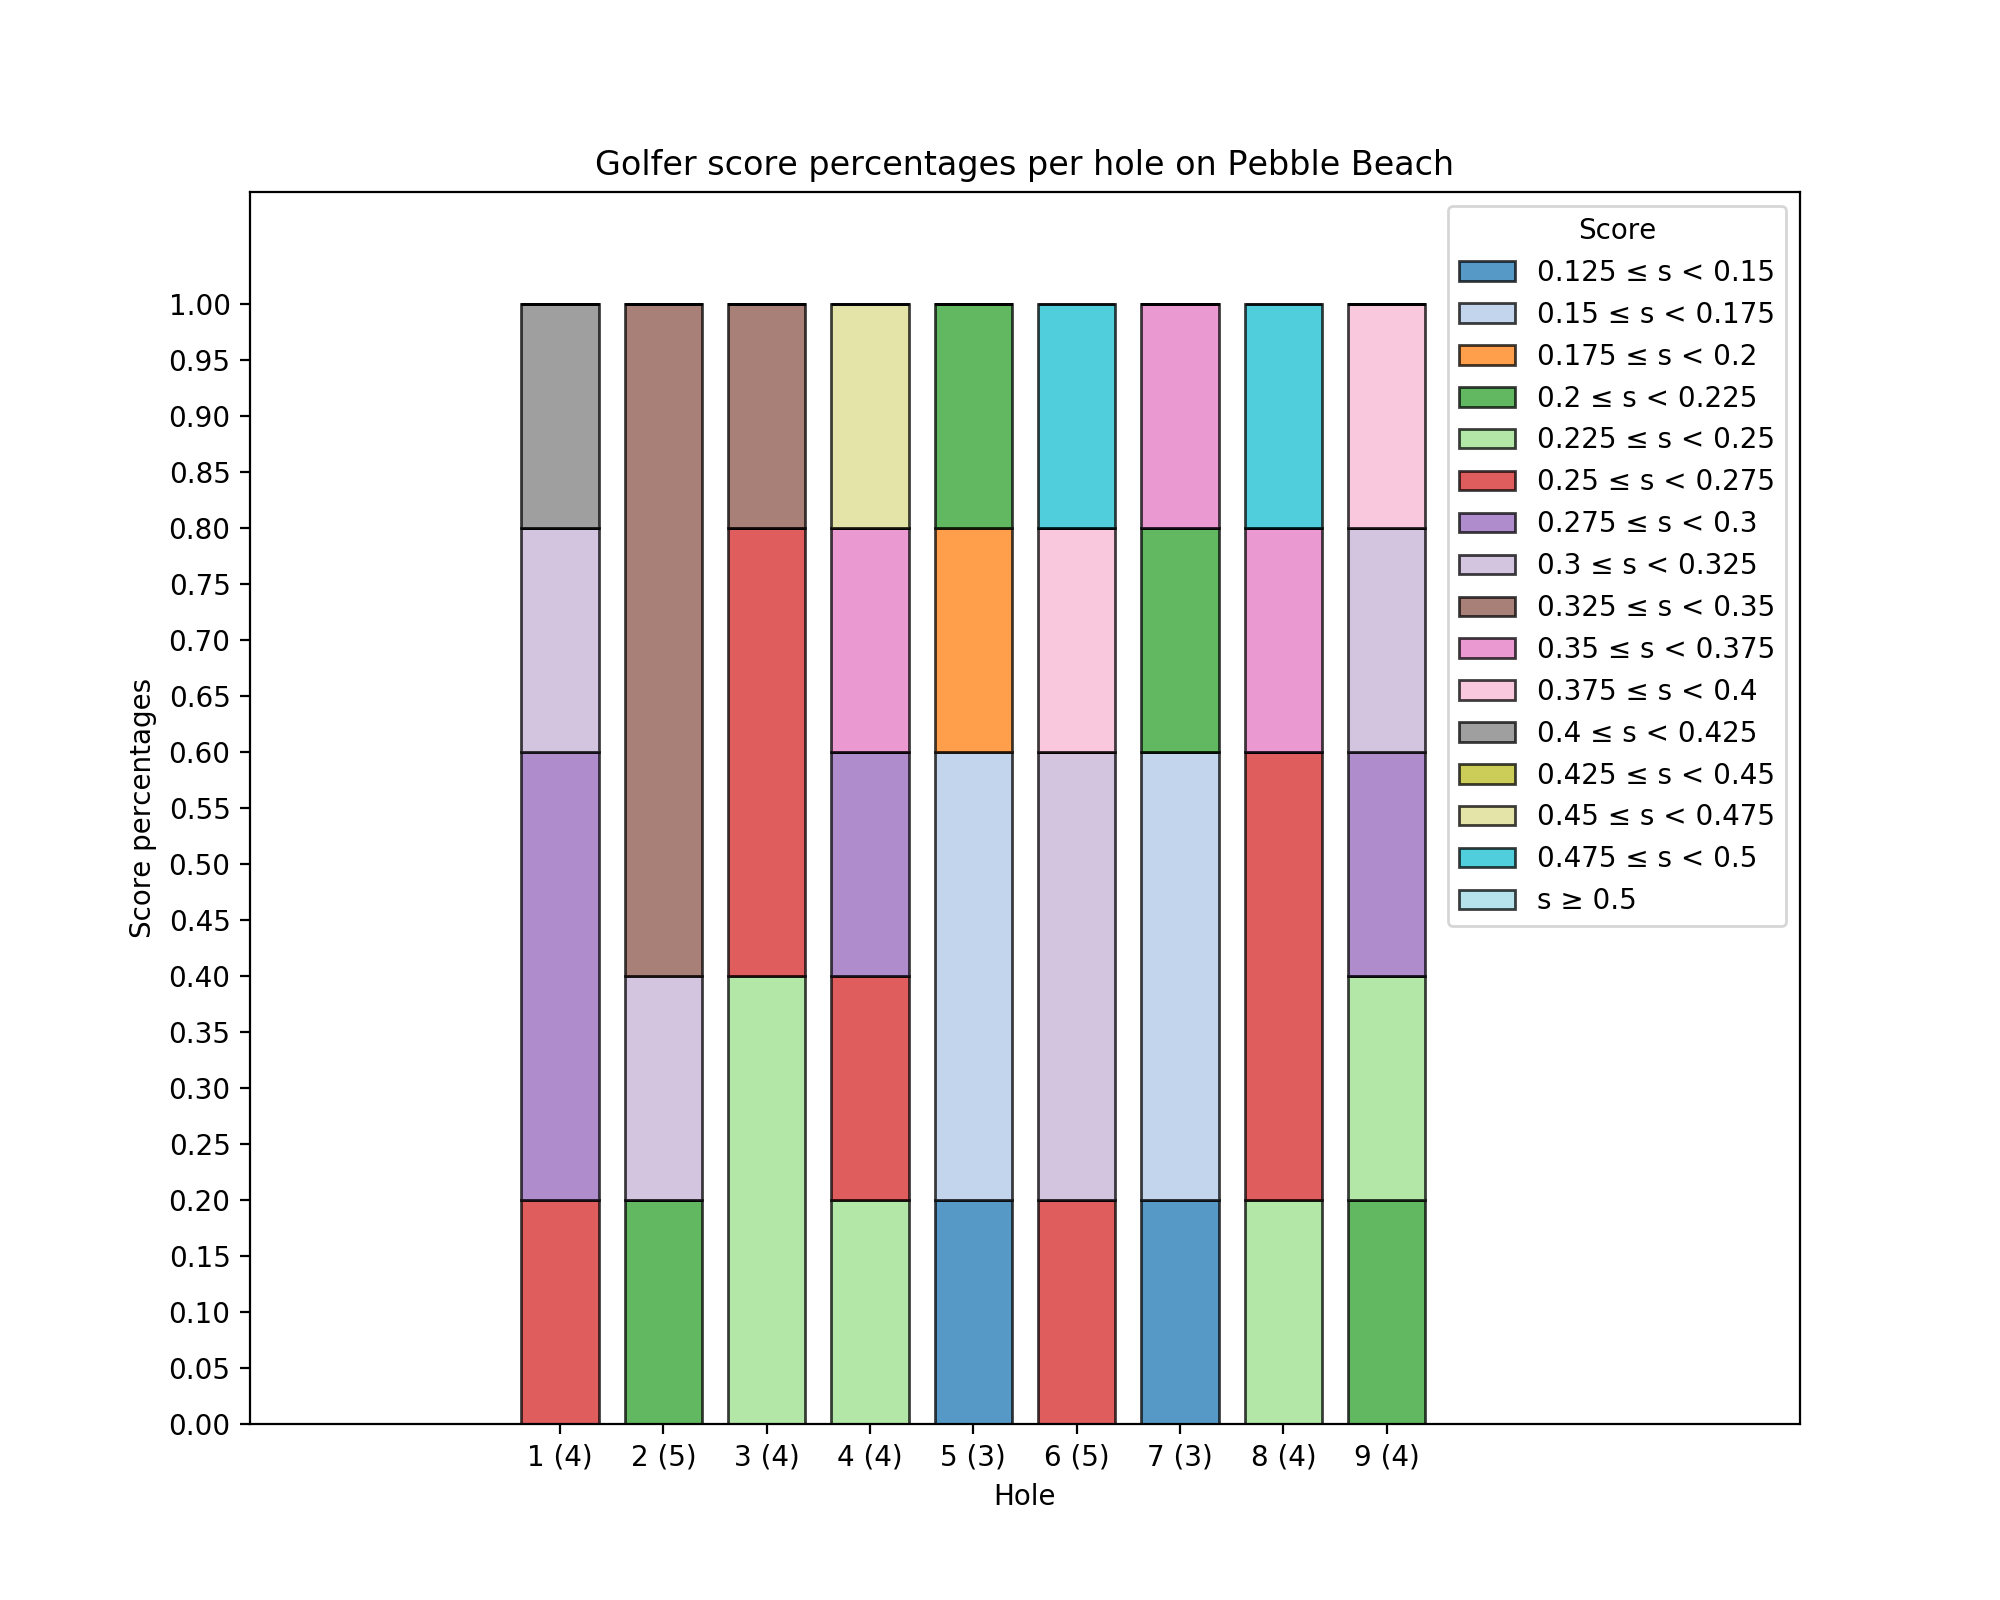
\includegraphics[height=0.3\textheight]{L2Percentages/L2_Score_Percentages_Pebble.png} 
    \end{subfigure}
    \begin{subfigure}{\textwidth}
    \centering
    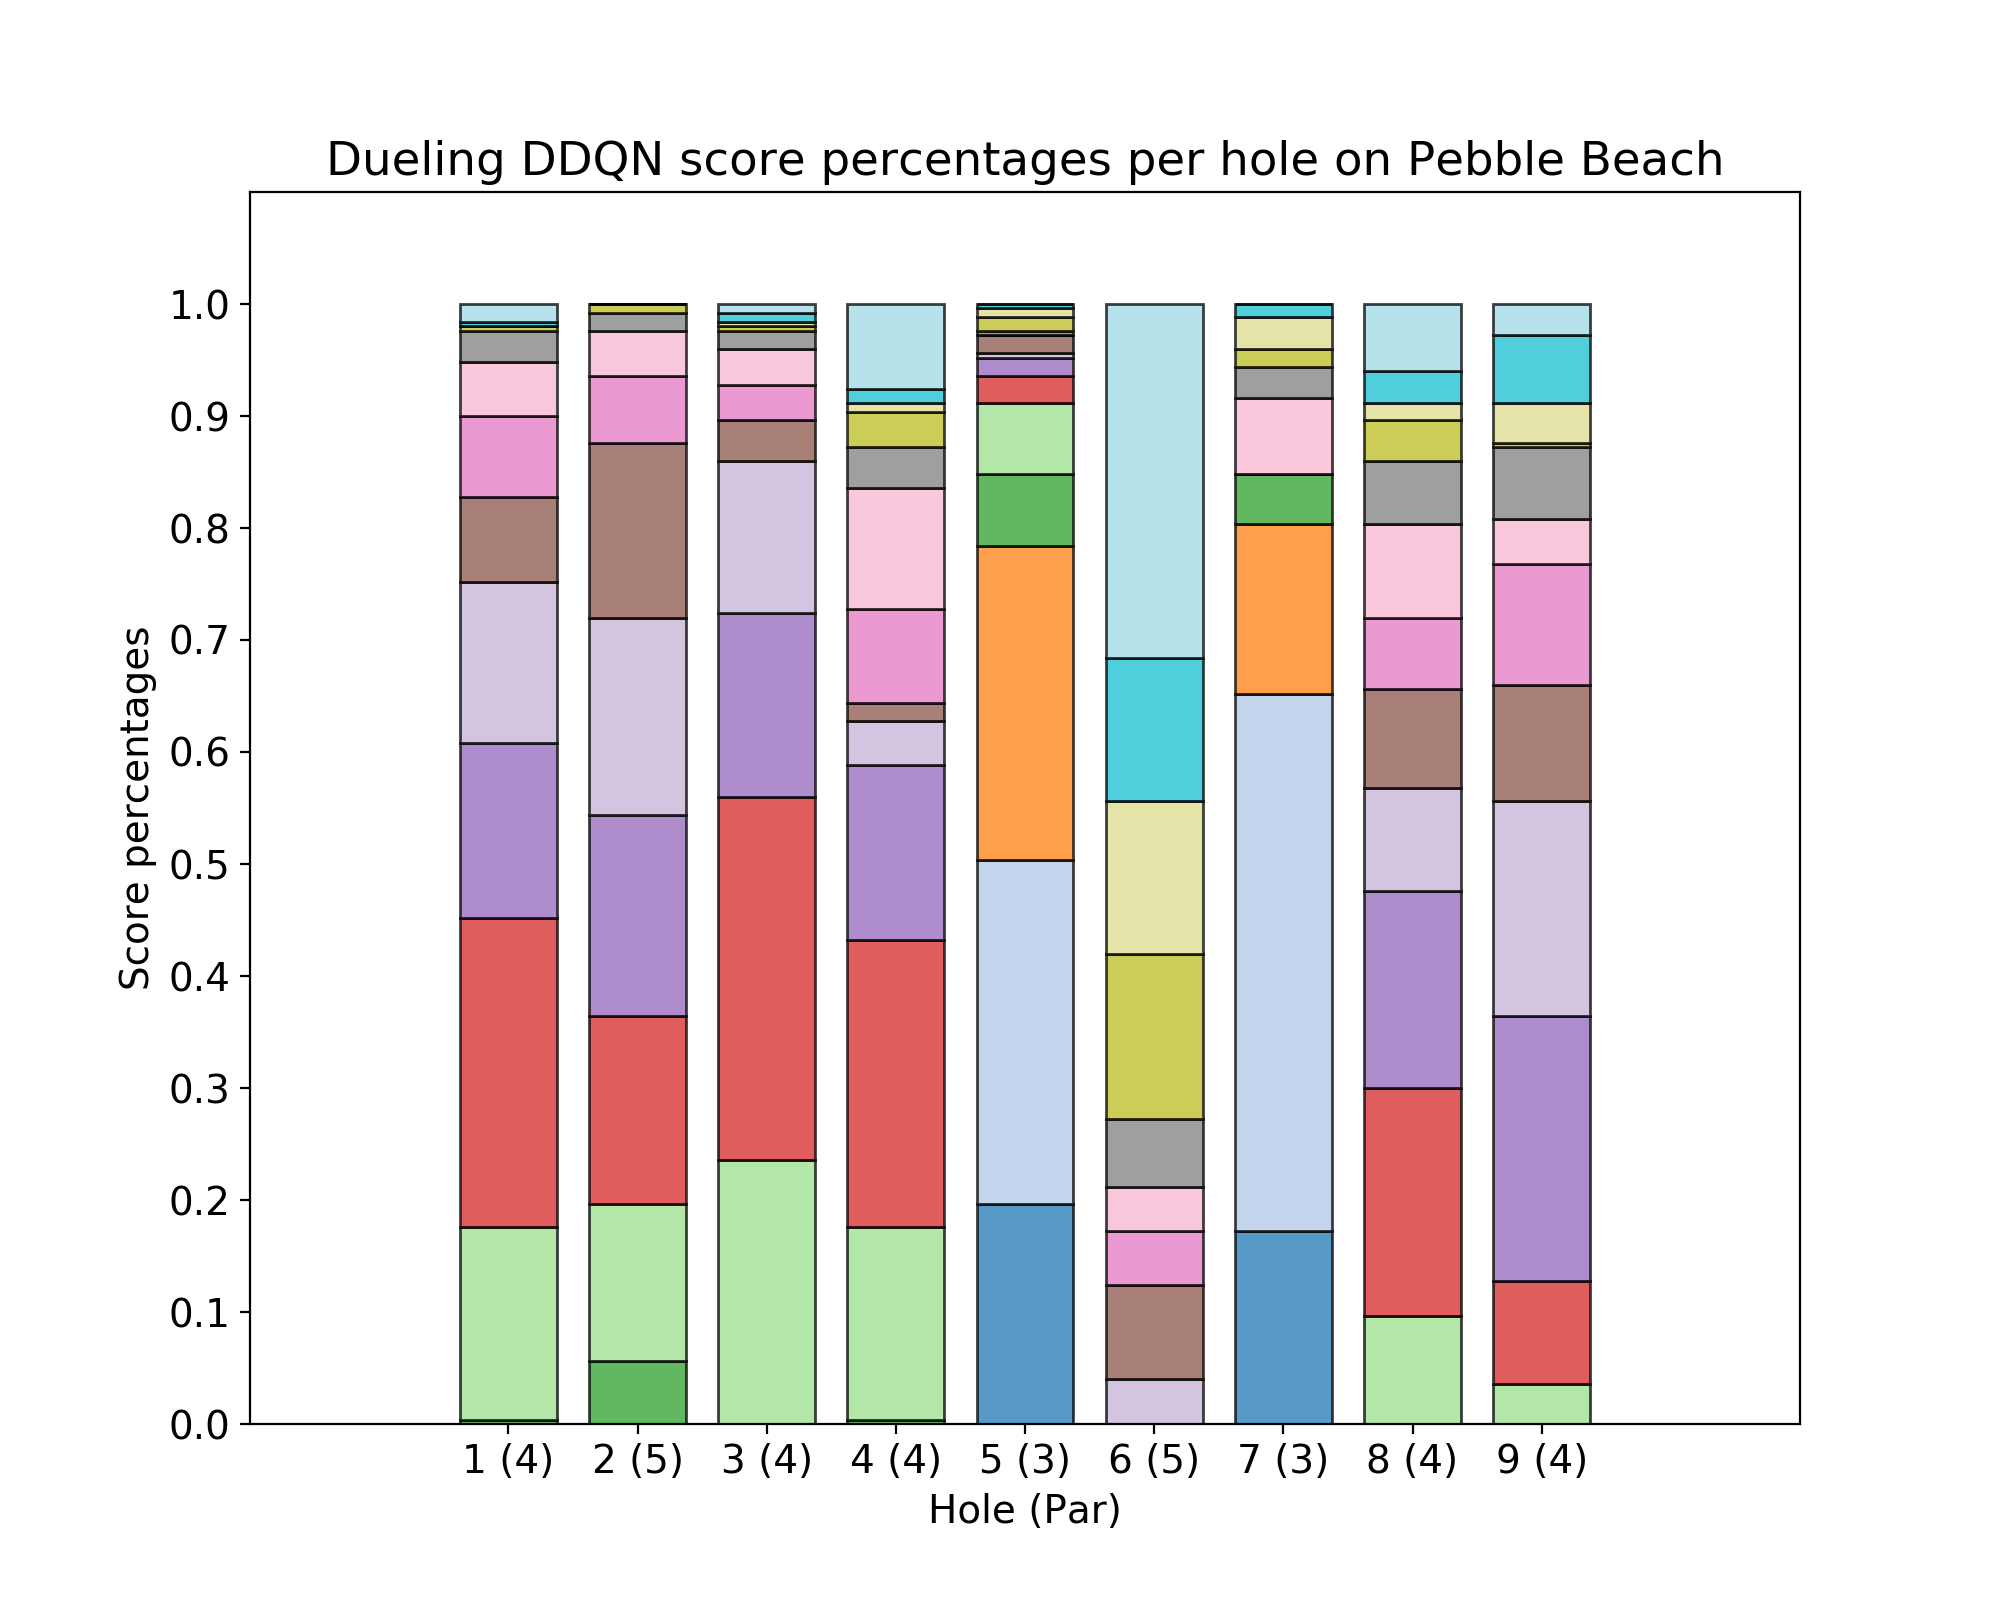
\includegraphics[height=0.3\textheight]{AgentPercentages/DDDQN_Score_Percentages_Pebble.png} 
    \end{subfigure}
    \begin{subfigure}{\textwidth}
    \centering
    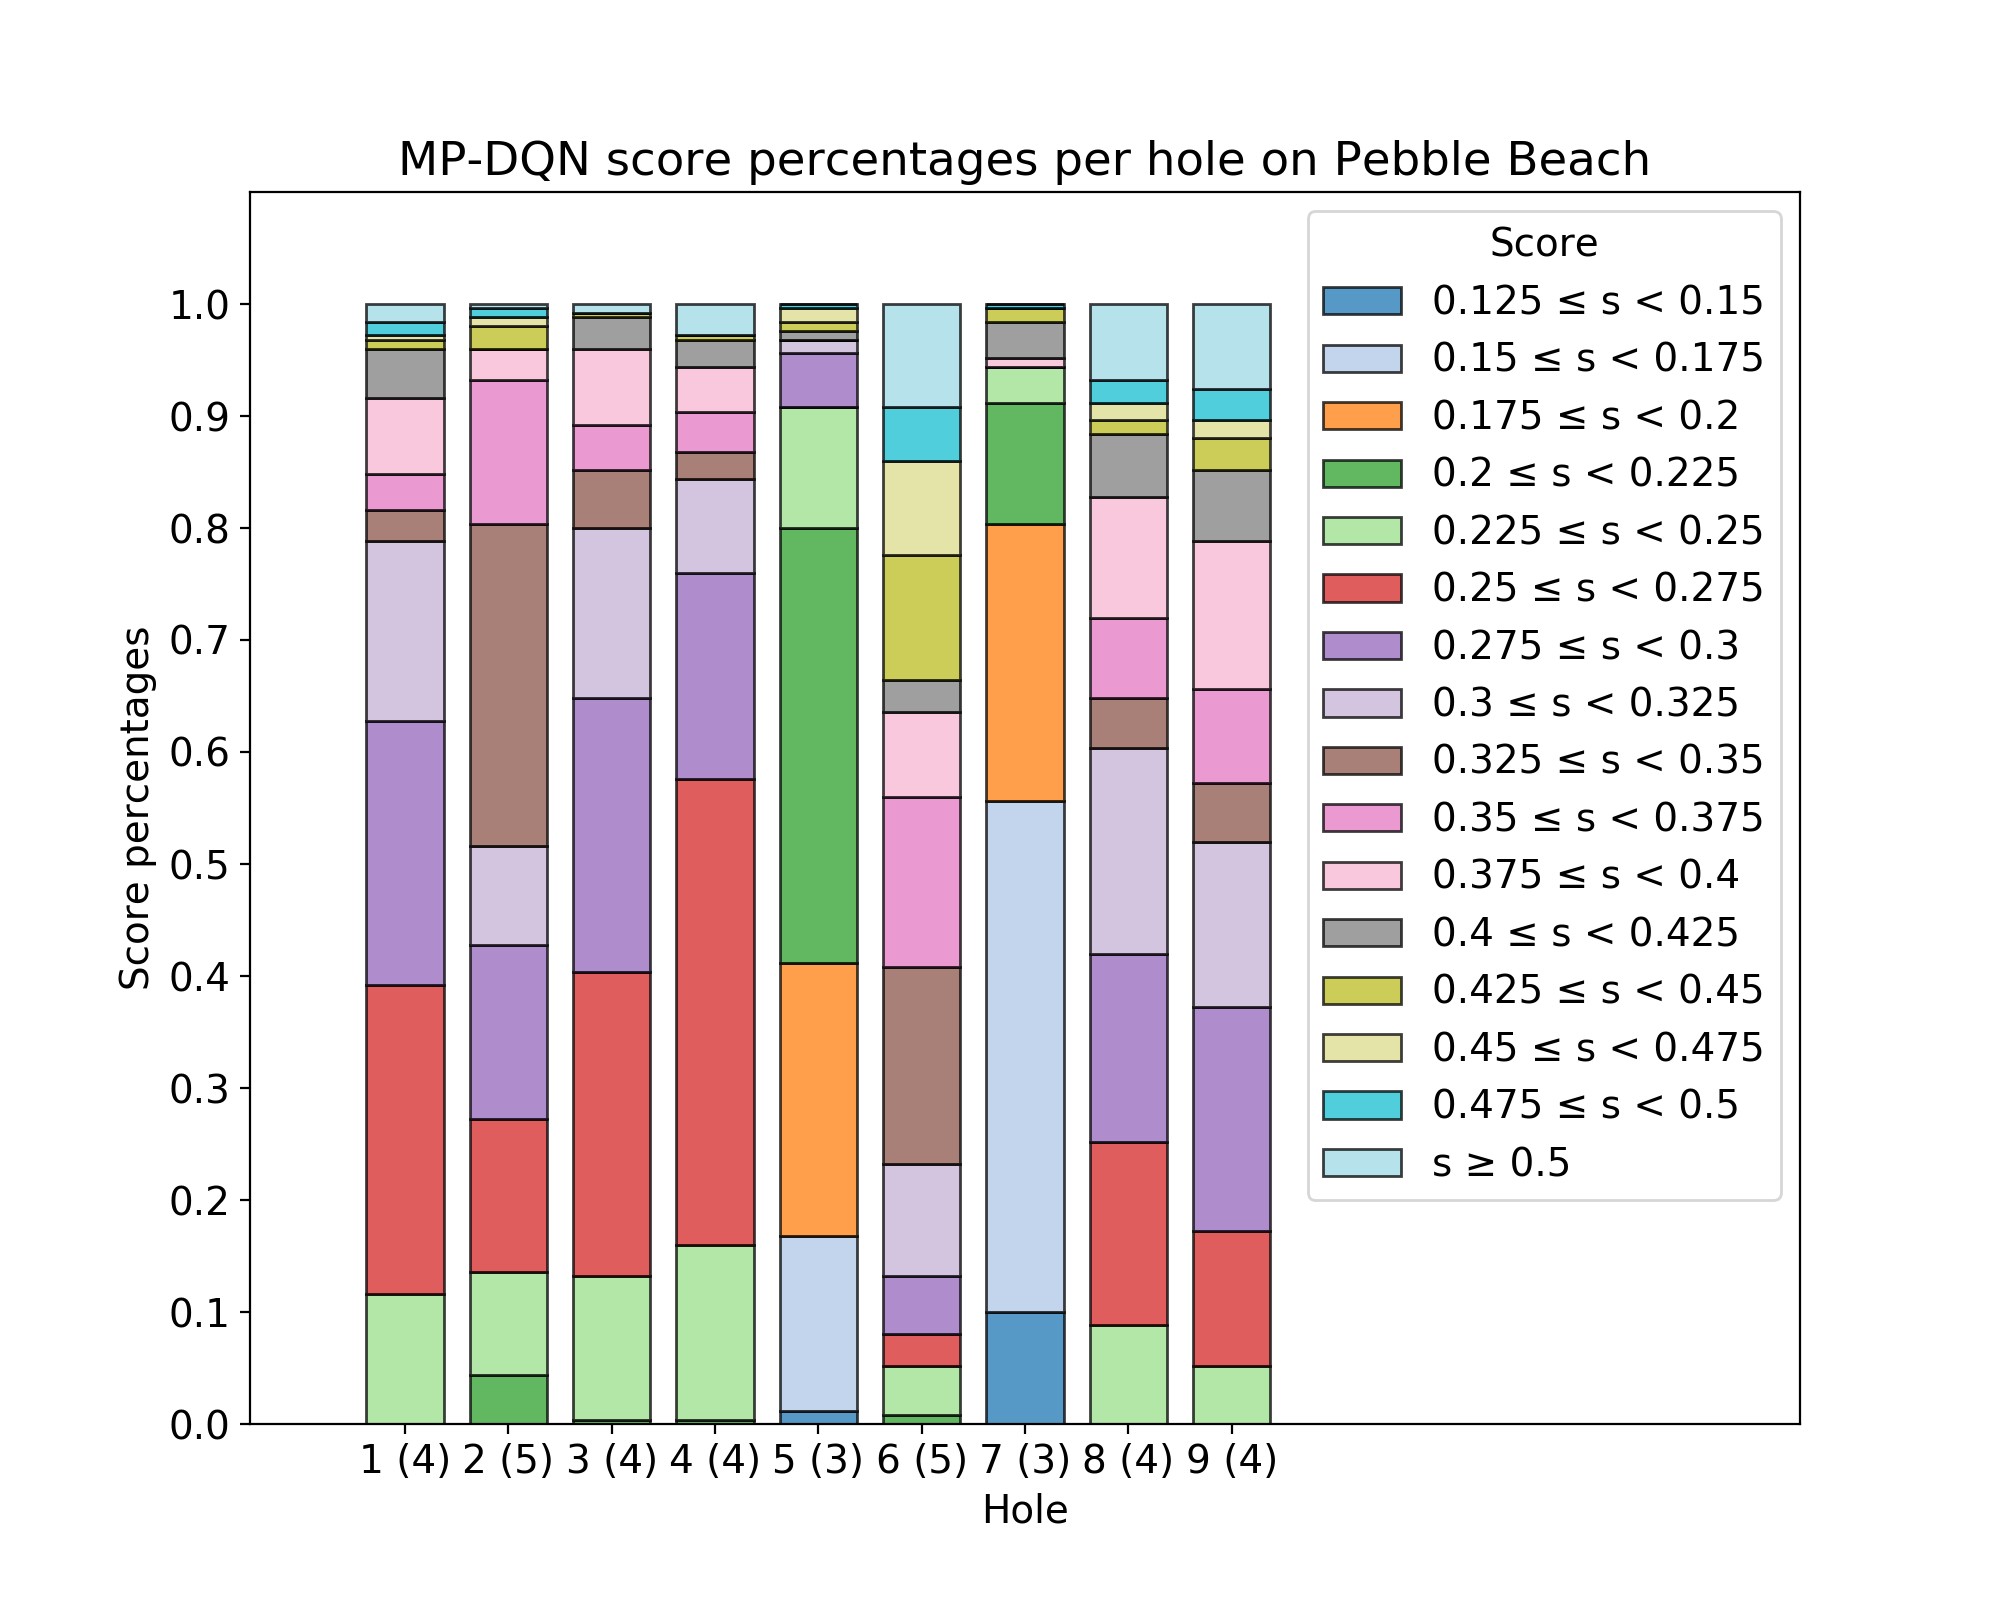
\includegraphics[height=0.3\textheight]{AgentPercentages/MPDQN_Score_Percentages_Pebble.png} 
    \end{subfigure}
    \caption{Histograms showcasing how often different scores were achieved on Pebble Beach by the golfer, Dueling DDQN agent and MP-DQN agent, respectively.}
    \label{fig:pebble_score_histograms}
\end{figure}

\begin{figure}
    \centering
    \begin{subfigure}{\textwidth}
    \centering
    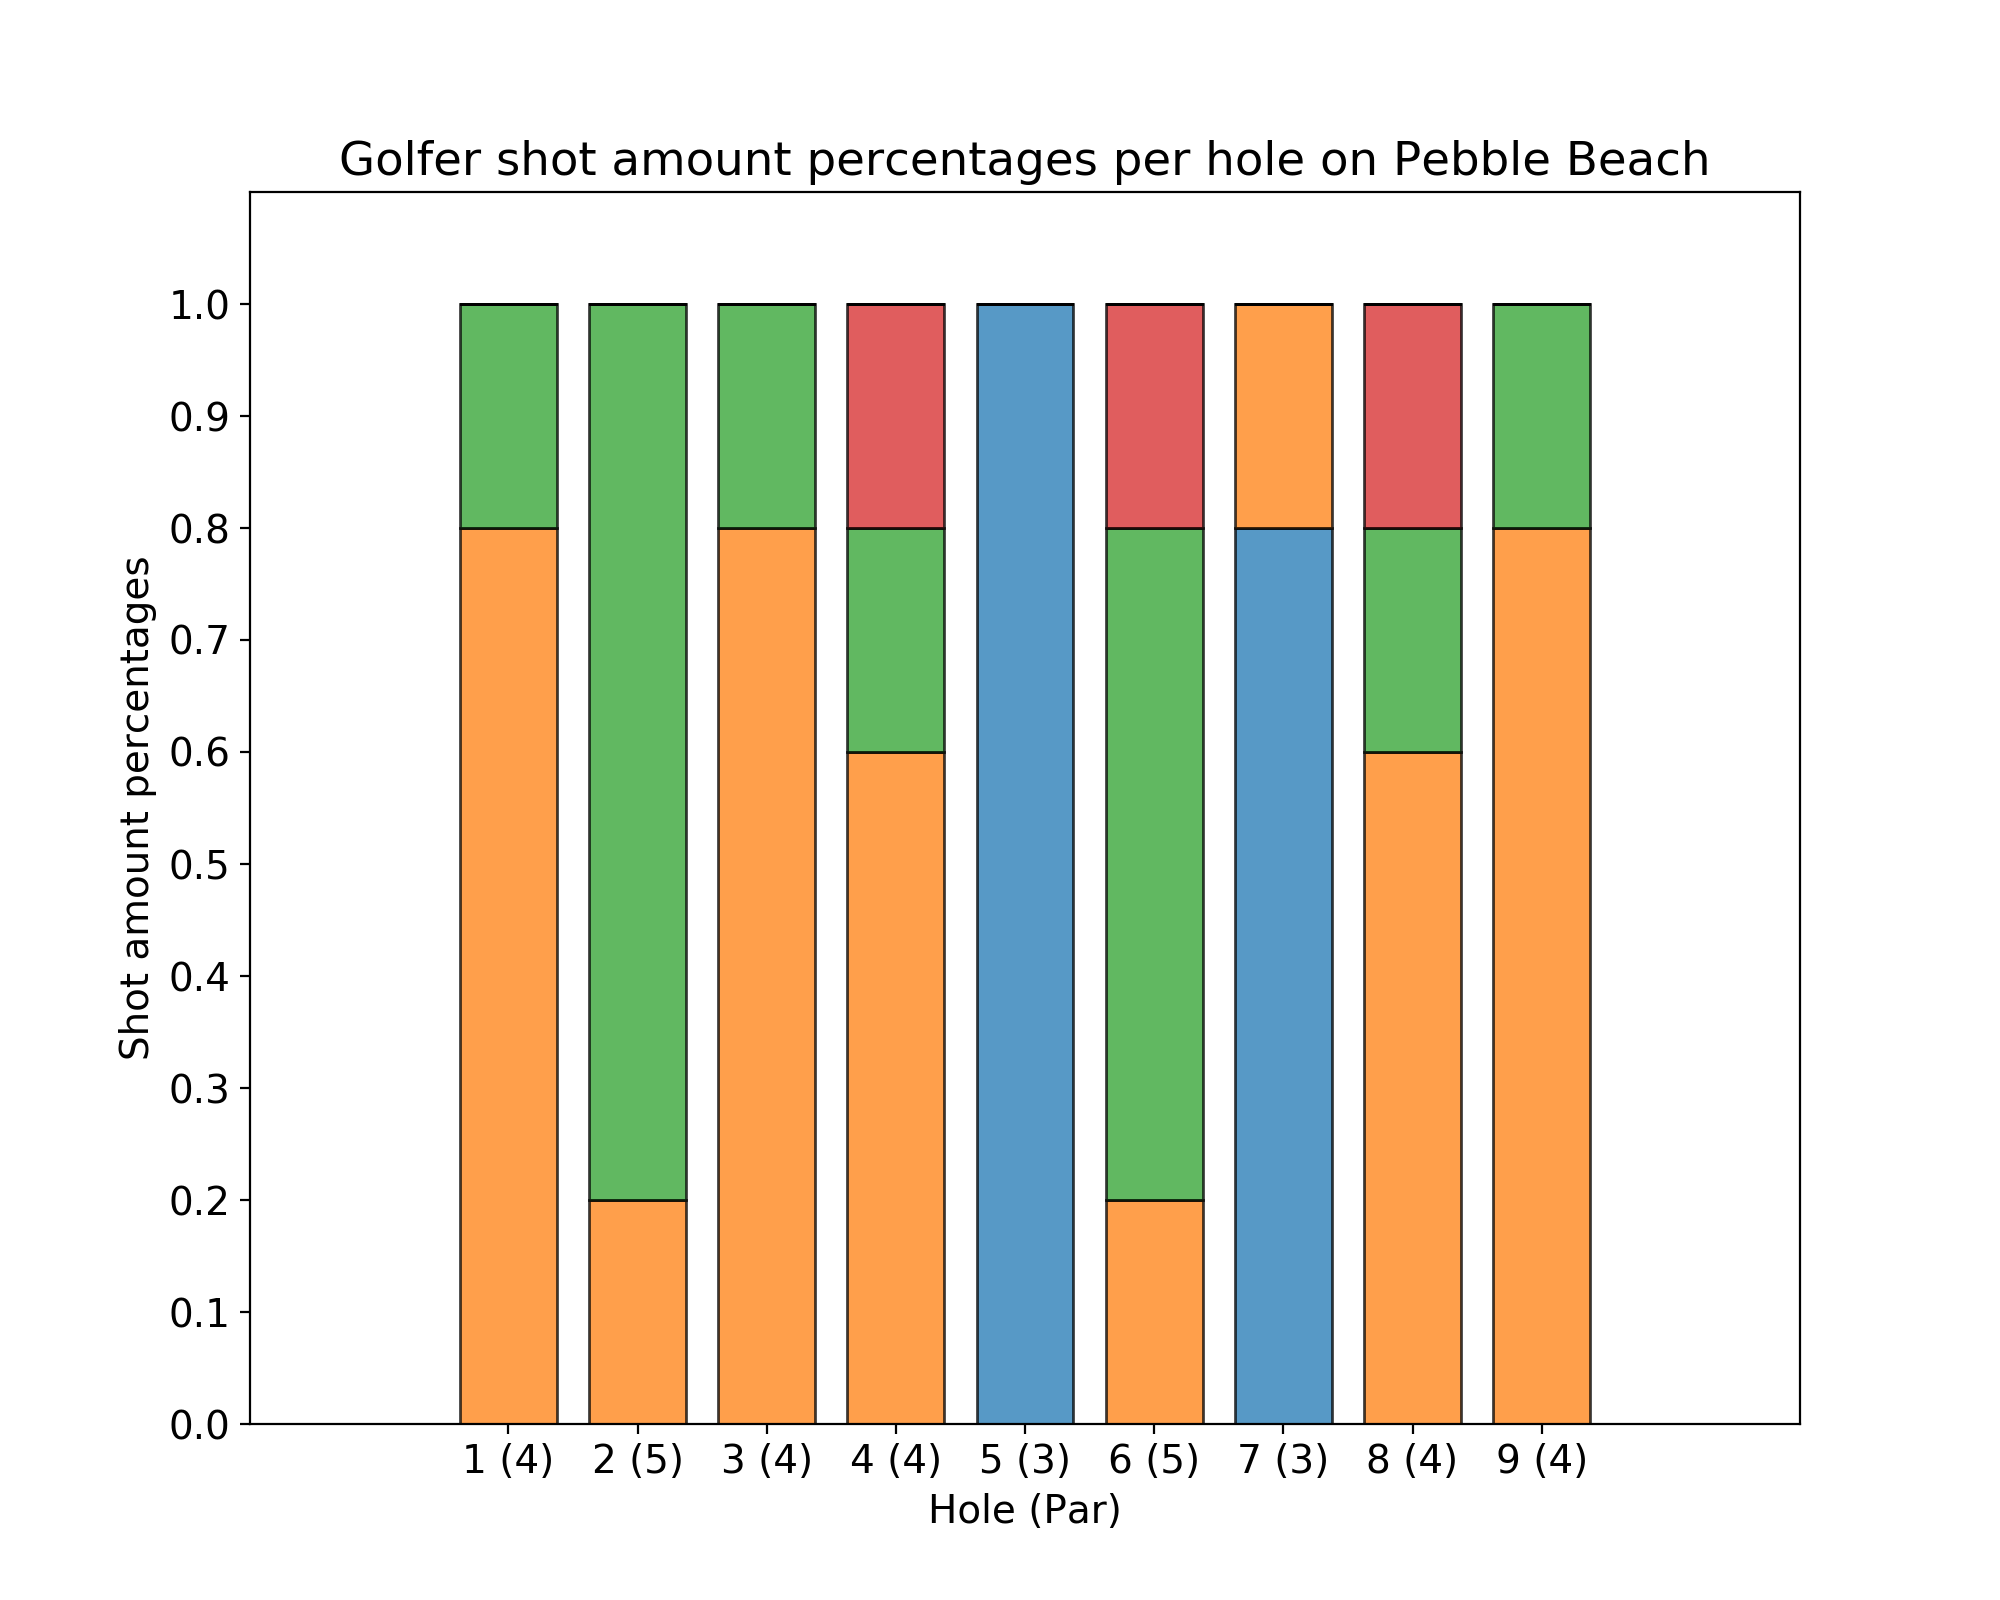
\includegraphics[height=0.3\textheight]{L2Percentages/L2_Shot_Percentages_Pebble.png} 
    \end{subfigure}
    \begin{subfigure}{\textwidth}
    \centering
    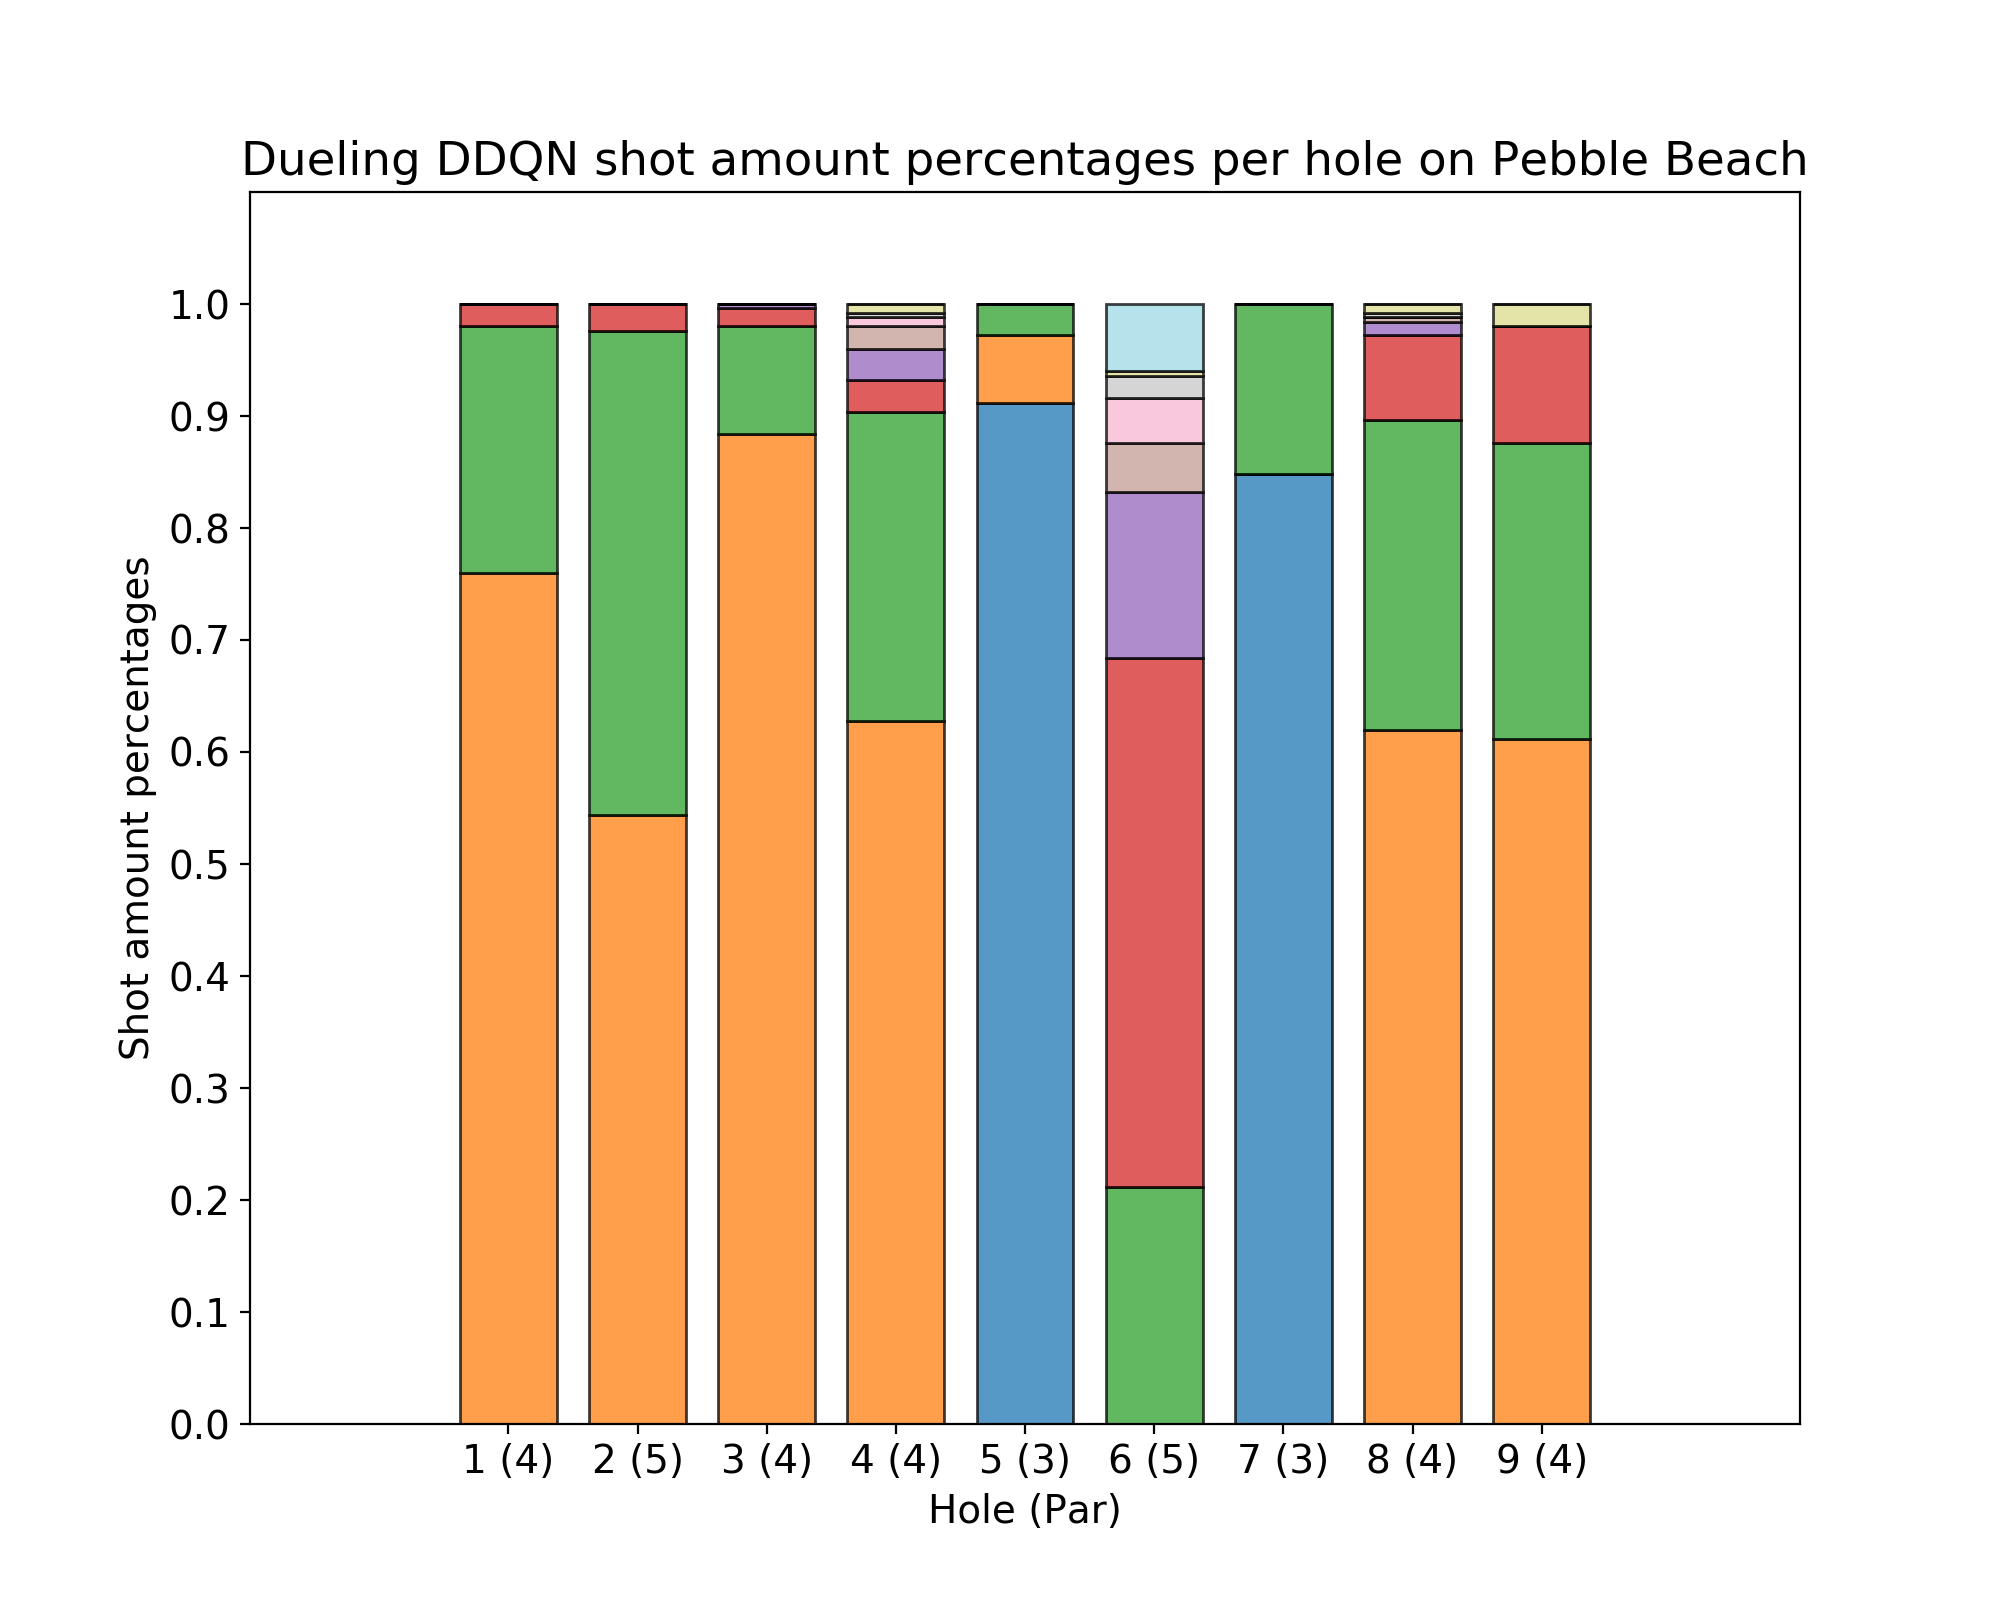
\includegraphics[height=0.3\textheight]{AgentPercentages/DDDQN_Shot_Percentages_Pebble.png} 
    \end{subfigure}
    \begin{subfigure}{\textwidth}
    \centering
    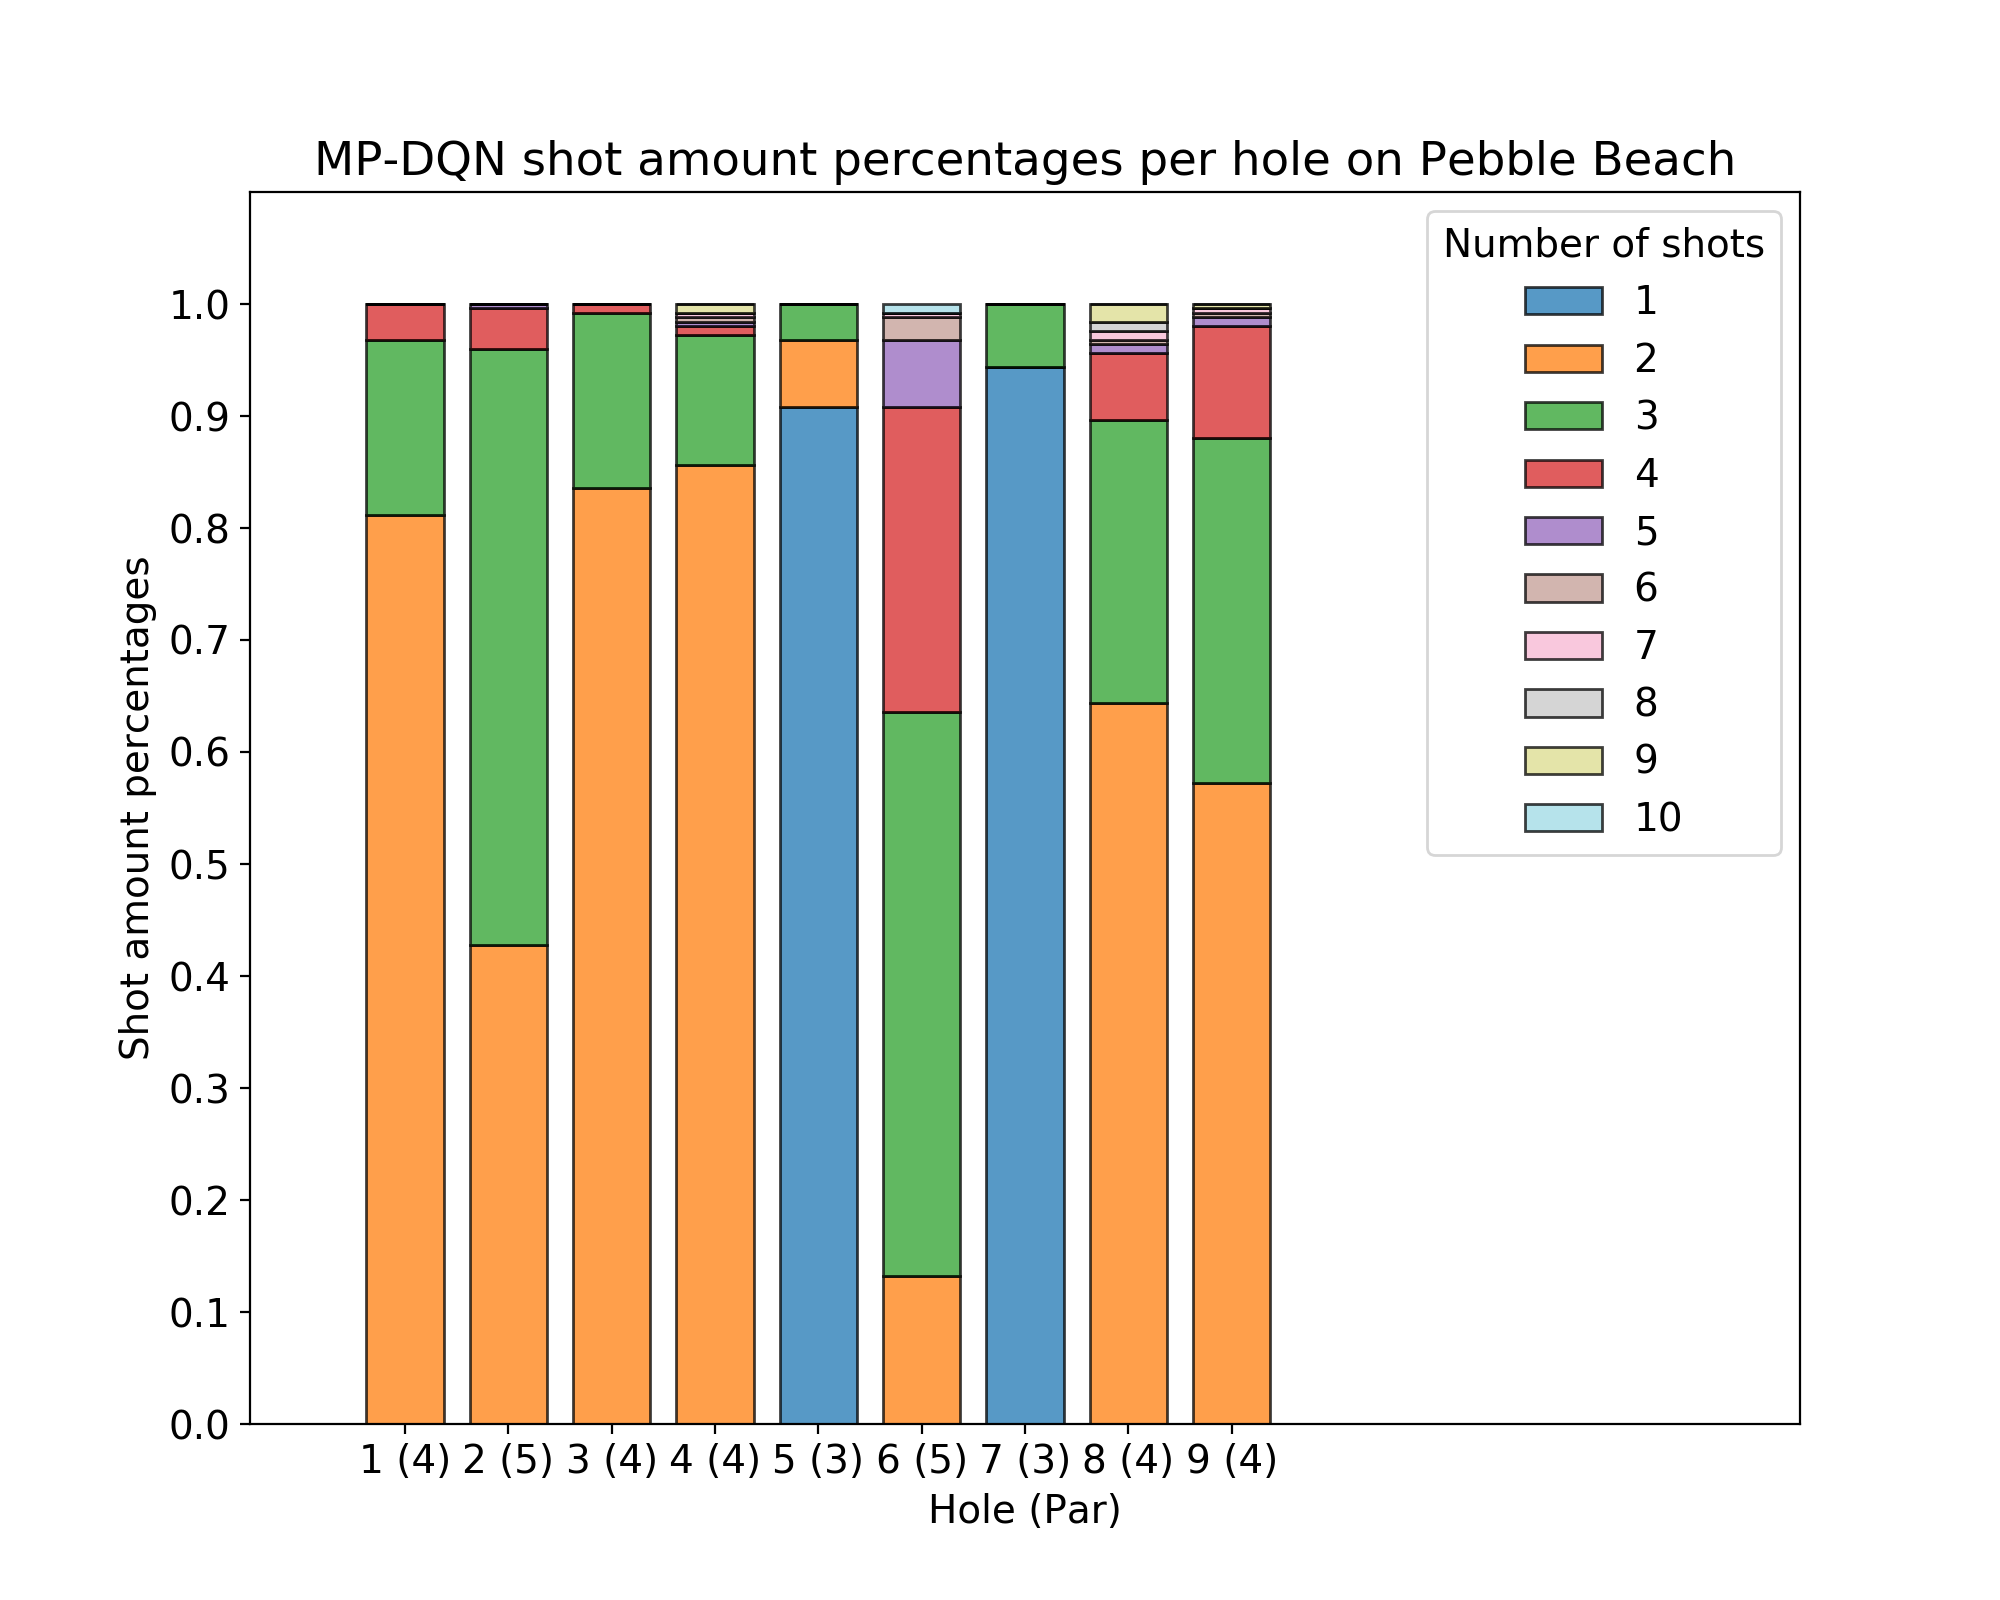
\includegraphics[height=0.3\textheight]{AgentPercentages/MPDQN_Shot_Percentages_Pebble.png} 
    \end{subfigure}
    \caption{Histograms showcasing how often different shot amounts were achieved on Pebble Beach by the golfer, Dueling DDQN agent and MP-DQN agent, respectively.}
    \label{fig:pebble_shot_histograms}
\end{figure}

\begin{figure}
    \centering
    \begin{subfigure}{\textwidth}
    \centering
    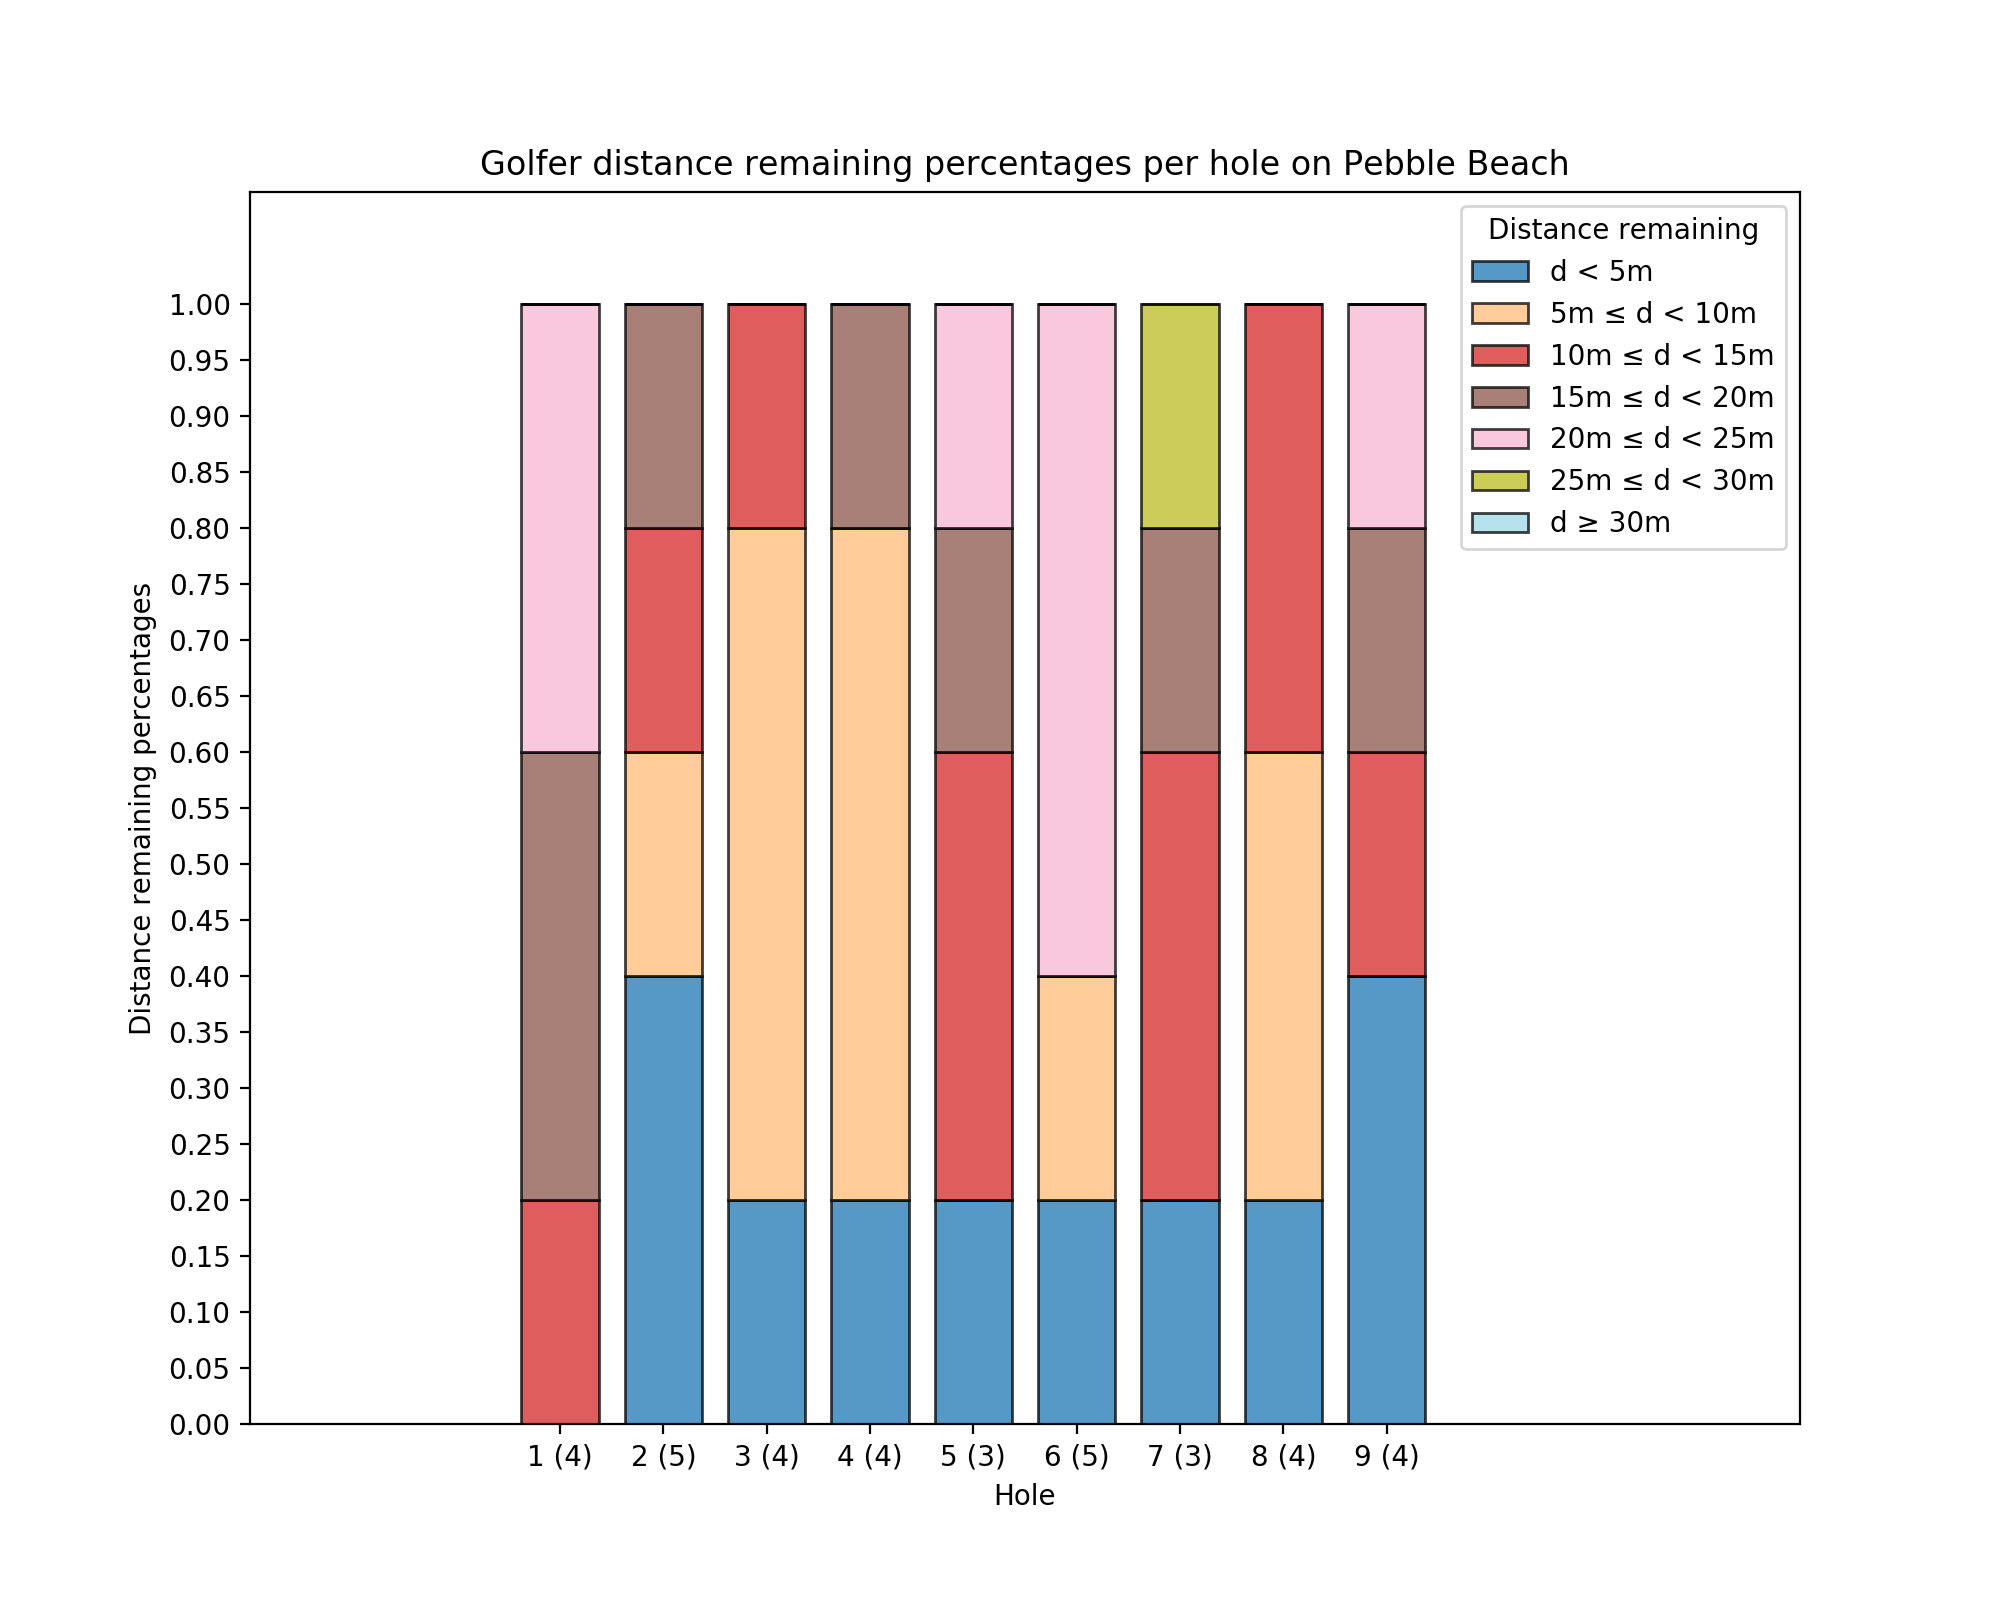
\includegraphics[height=0.3\textheight]{L2Percentages/L2_Distance_Percentages_Pebble.png} 
    \end{subfigure}
    \begin{subfigure}{\textwidth}
    \centering
    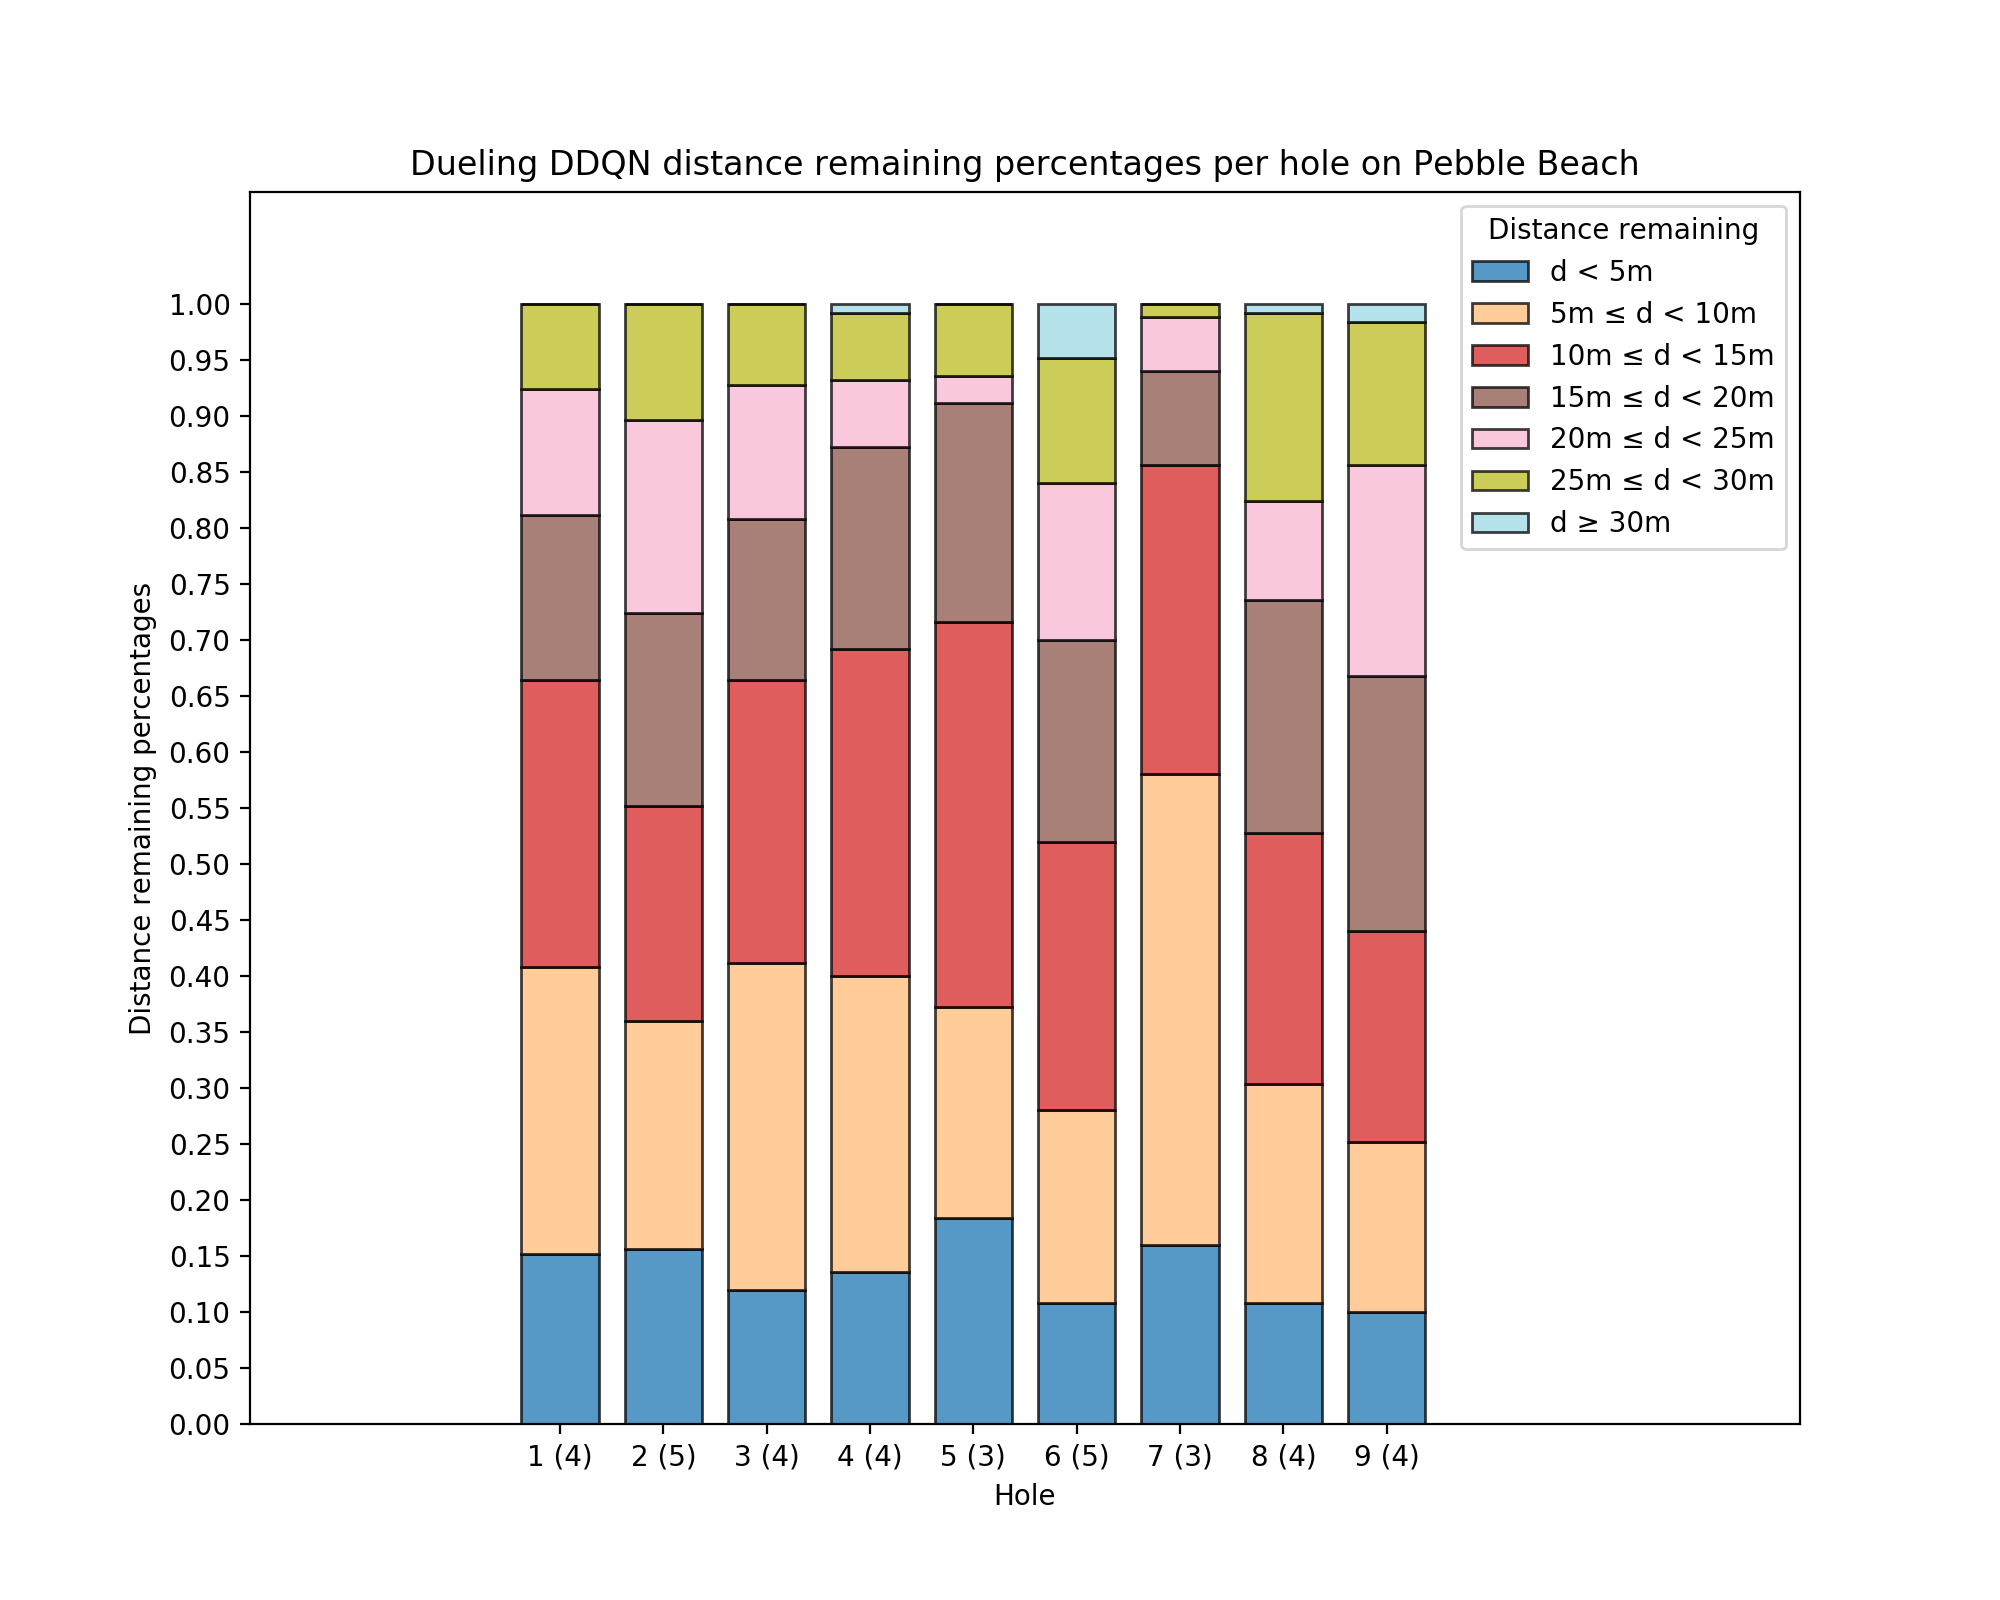
\includegraphics[height=0.3\textheight]{AgentPercentages/DDDQN_Distance_Percentages_Pebble.png} 
    \end{subfigure}
    \begin{subfigure}{\textwidth}
    \centering
    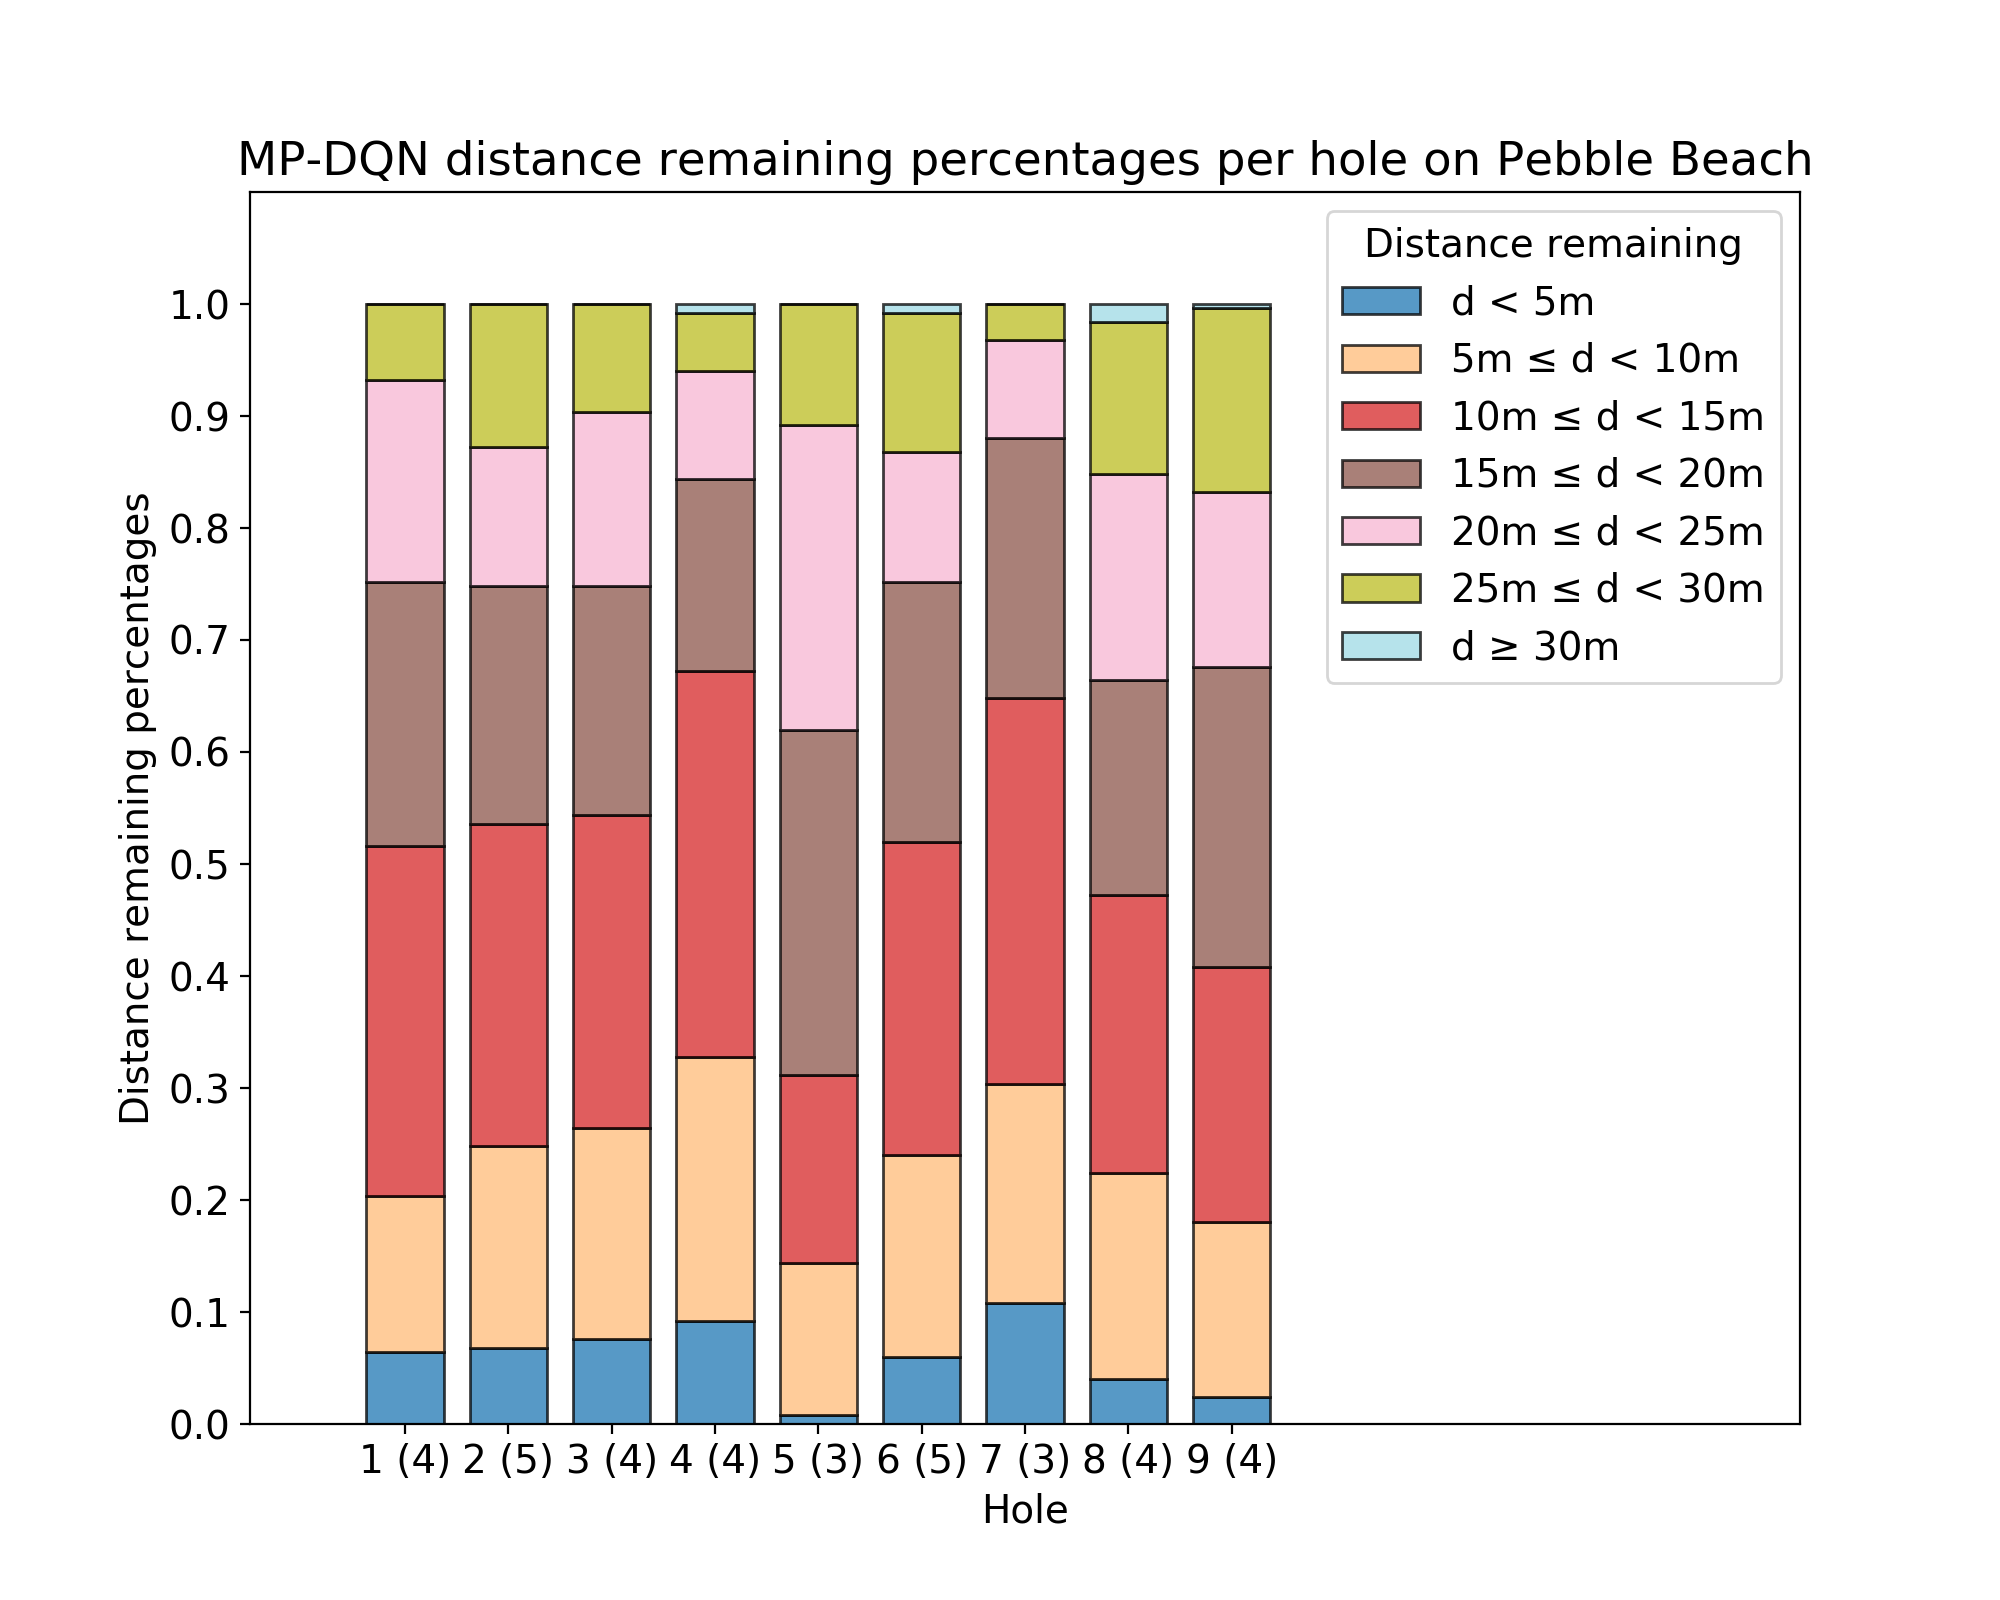
\includegraphics[height=0.3\textheight]{AgentPercentages/MPDQN_Distance_Percentages_Pebble.png} 
    \end{subfigure}
    \caption{Histograms showcasing how often different distances remaining were achieved on Pebble Beach by the golfer, Dueling DDQN agent and MP-DQN agent, respectively.}
    \label{fig:pebble_distance_histograms}
\end{figure}

\chapter{Pebble Beach Club Choices}
\label{app:pebble_club_choices}
\begin{figure}
    \centering
    \begin{subfigure}{\textwidth}
    \centering
    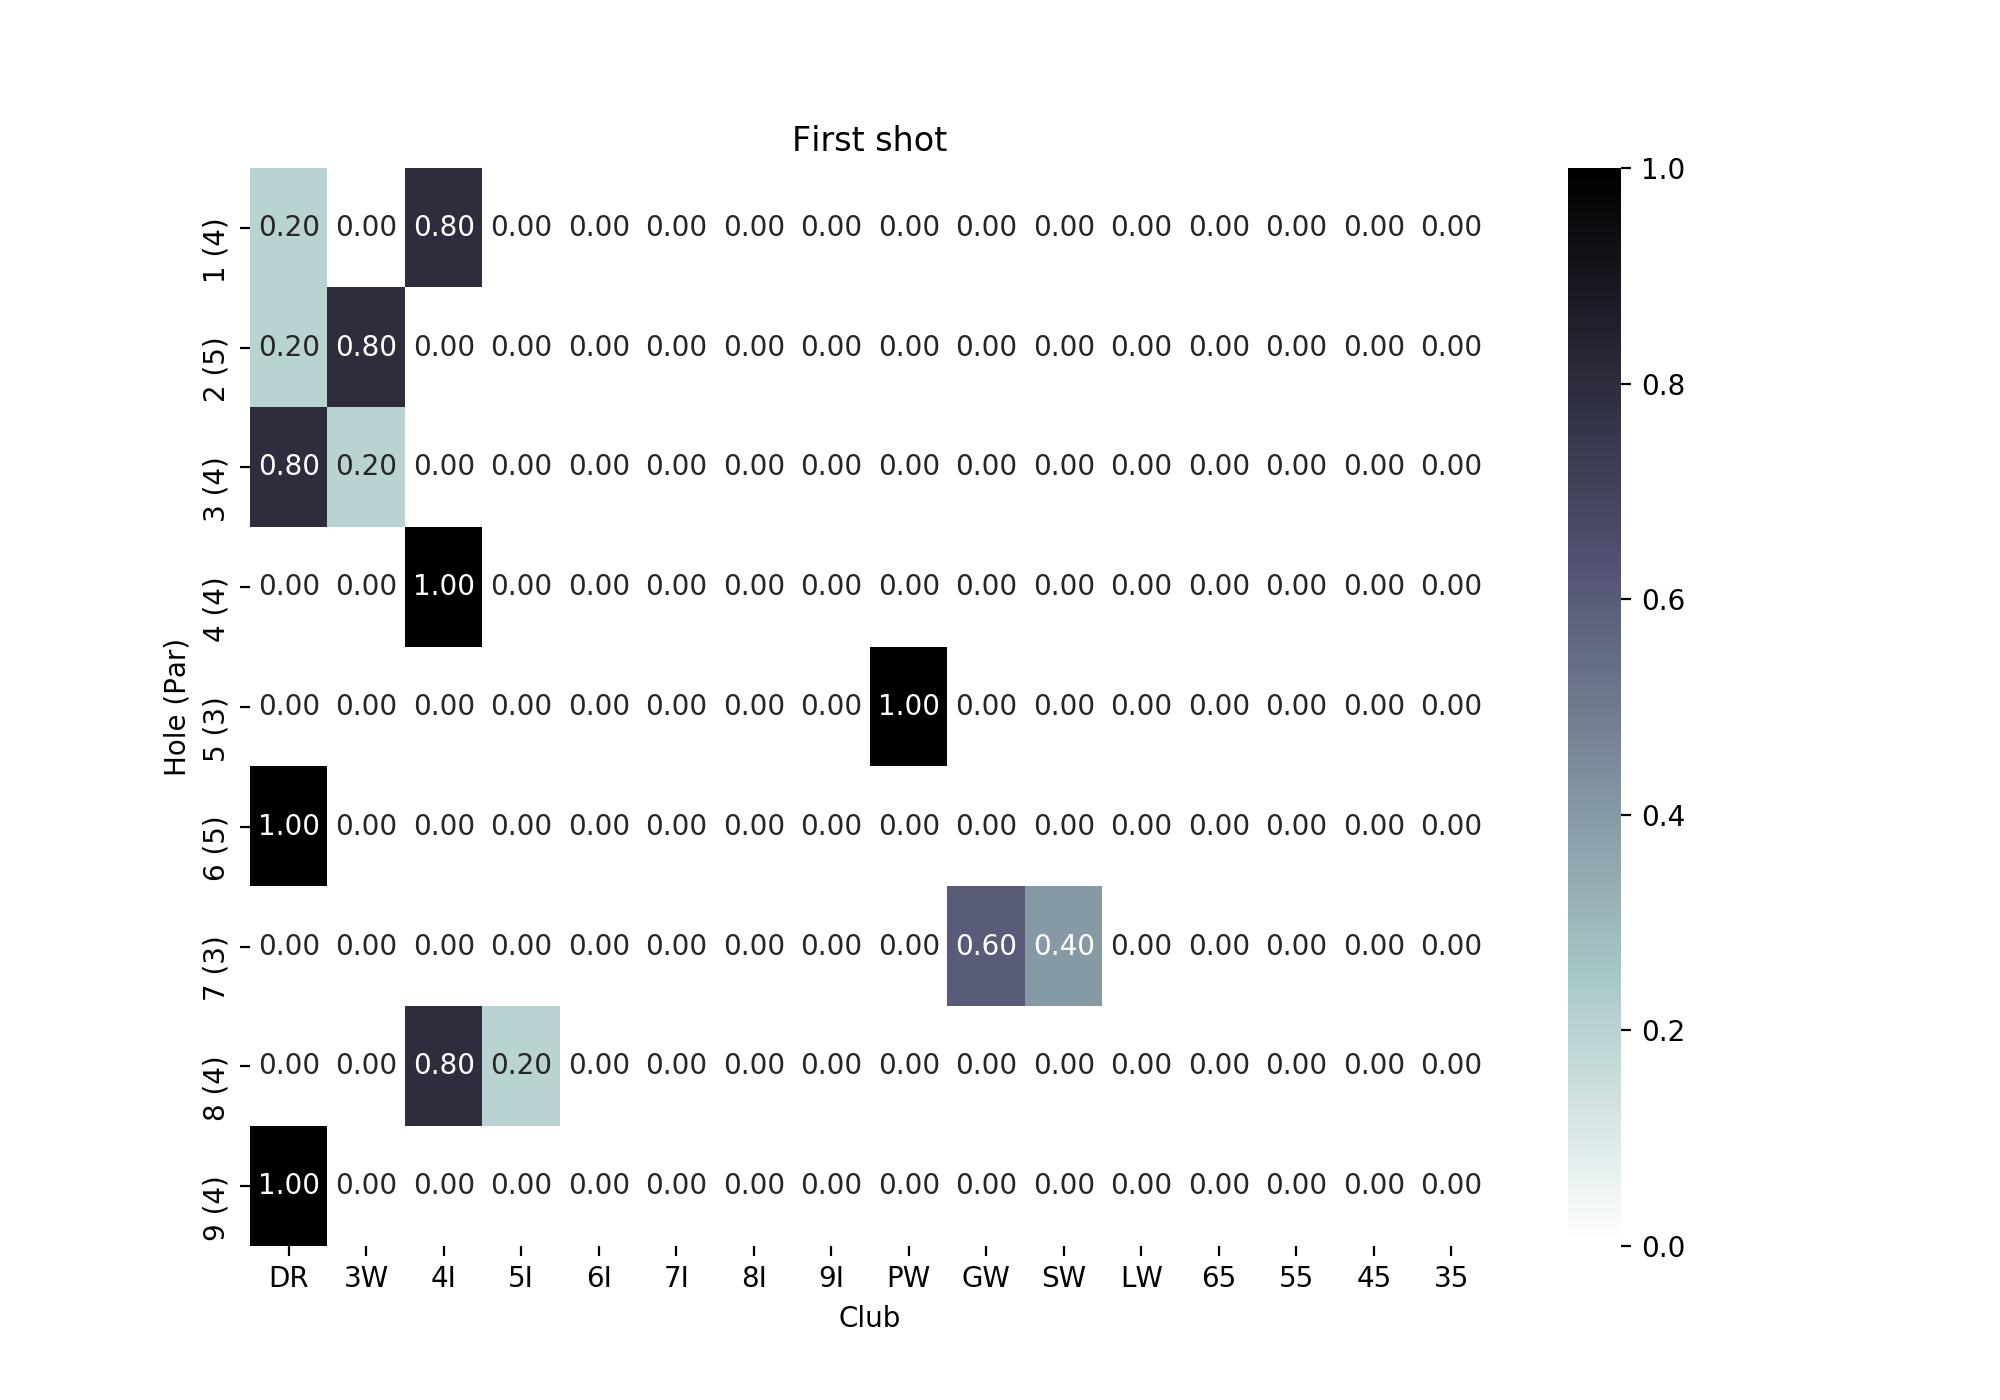
\includegraphics[height=0.3\textheight]{L2ClubChoices/Ludvig_Pebble_Club_Choices_First_Shot.png} 
    \end{subfigure}
    \begin{subfigure}{\textwidth}
    \centering
    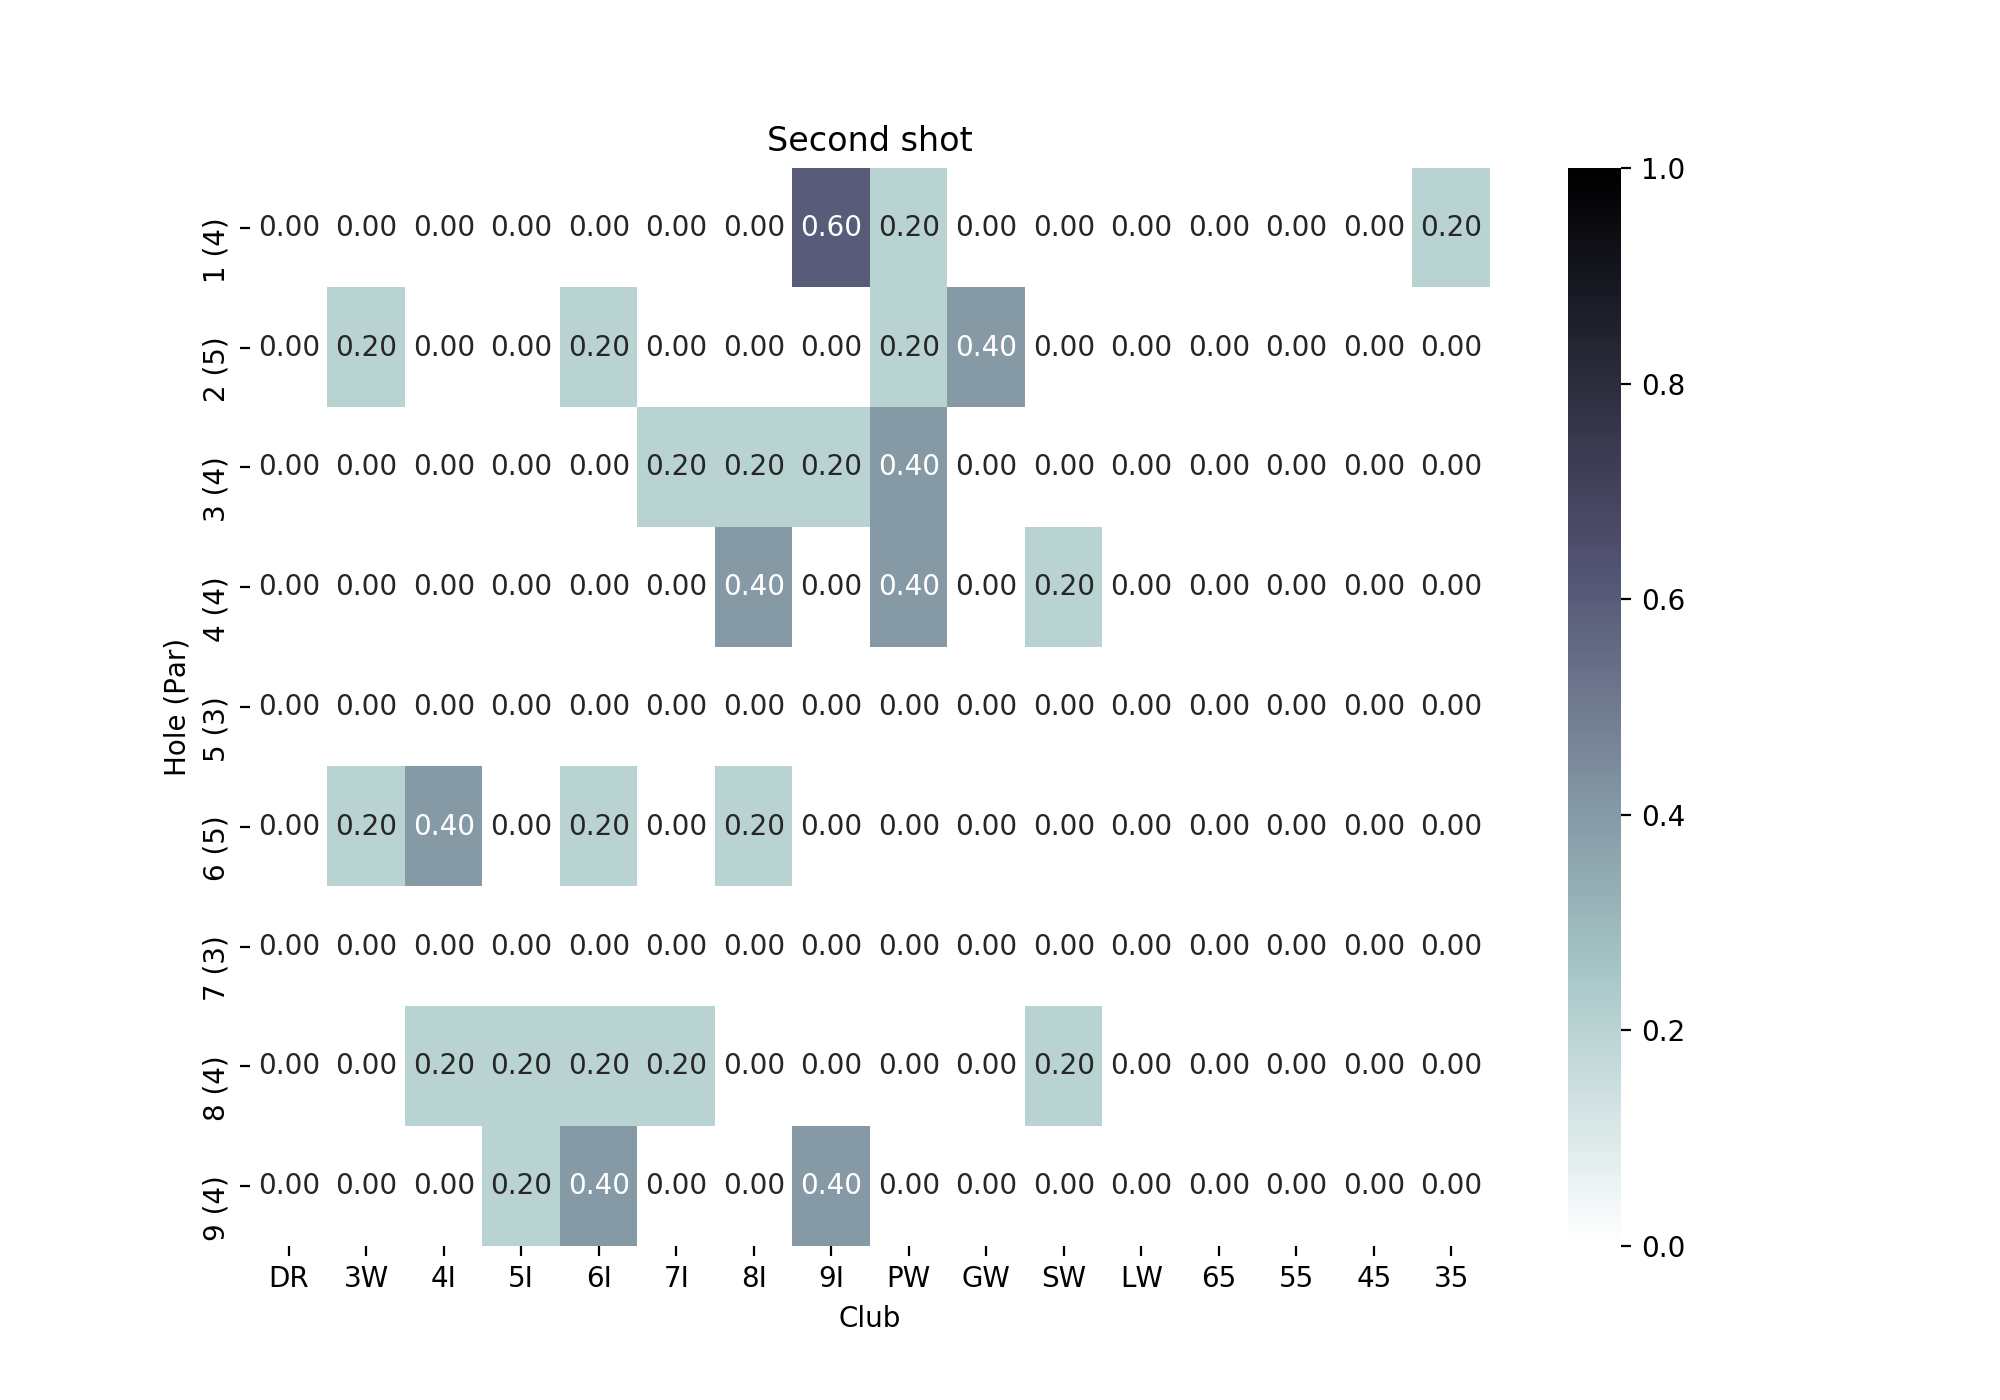
\includegraphics[height=0.3\textheight]{L2ClubChoices/Ludvig_Pebble_Club_Choices_Second_Shot.png} 
    \end{subfigure}
    \begin{subfigure}{\textwidth}
    \centering
    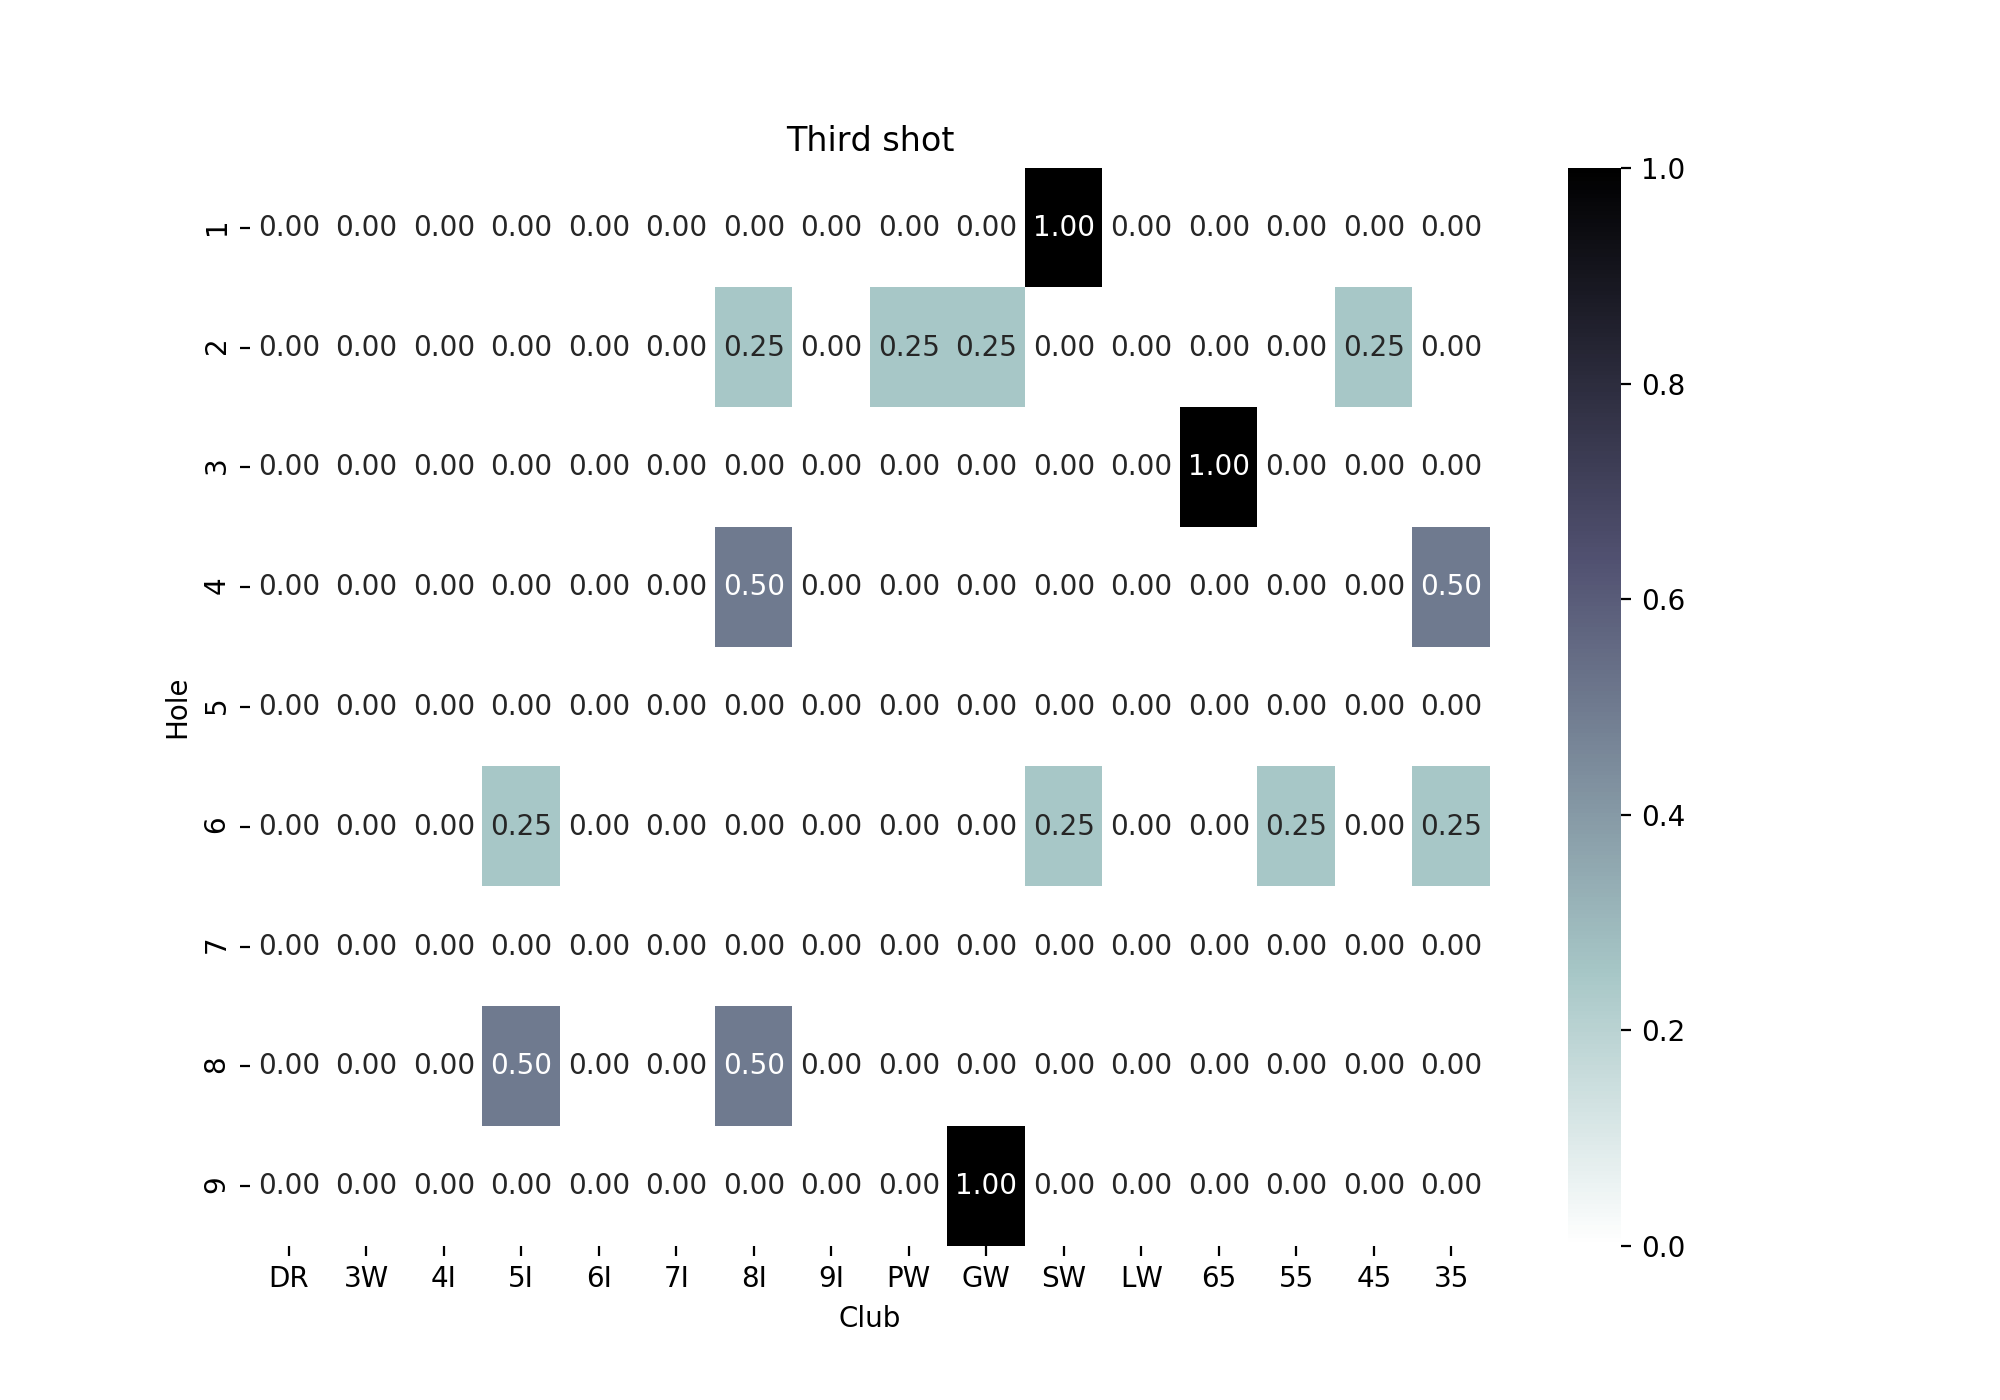
\includegraphics[height=0.3\textheight]{L2ClubChoices/Ludvig_Pebble_Club_Choices_Third_Shot.png} 
    \end{subfigure}
    \caption{Confusion matrices indicating how often clubs were chosen by the golfer for the first, second and third shot on a given hole at Pebble Beach. Only the first three shots are shown because most of the holes played were completed within this shot range.}
    \label{fig:L2_pebble_club_choice_confusion}
\end{figure}

\begin{figure}
    \centering
    \begin{subfigure}{\textwidth}
    \centering
    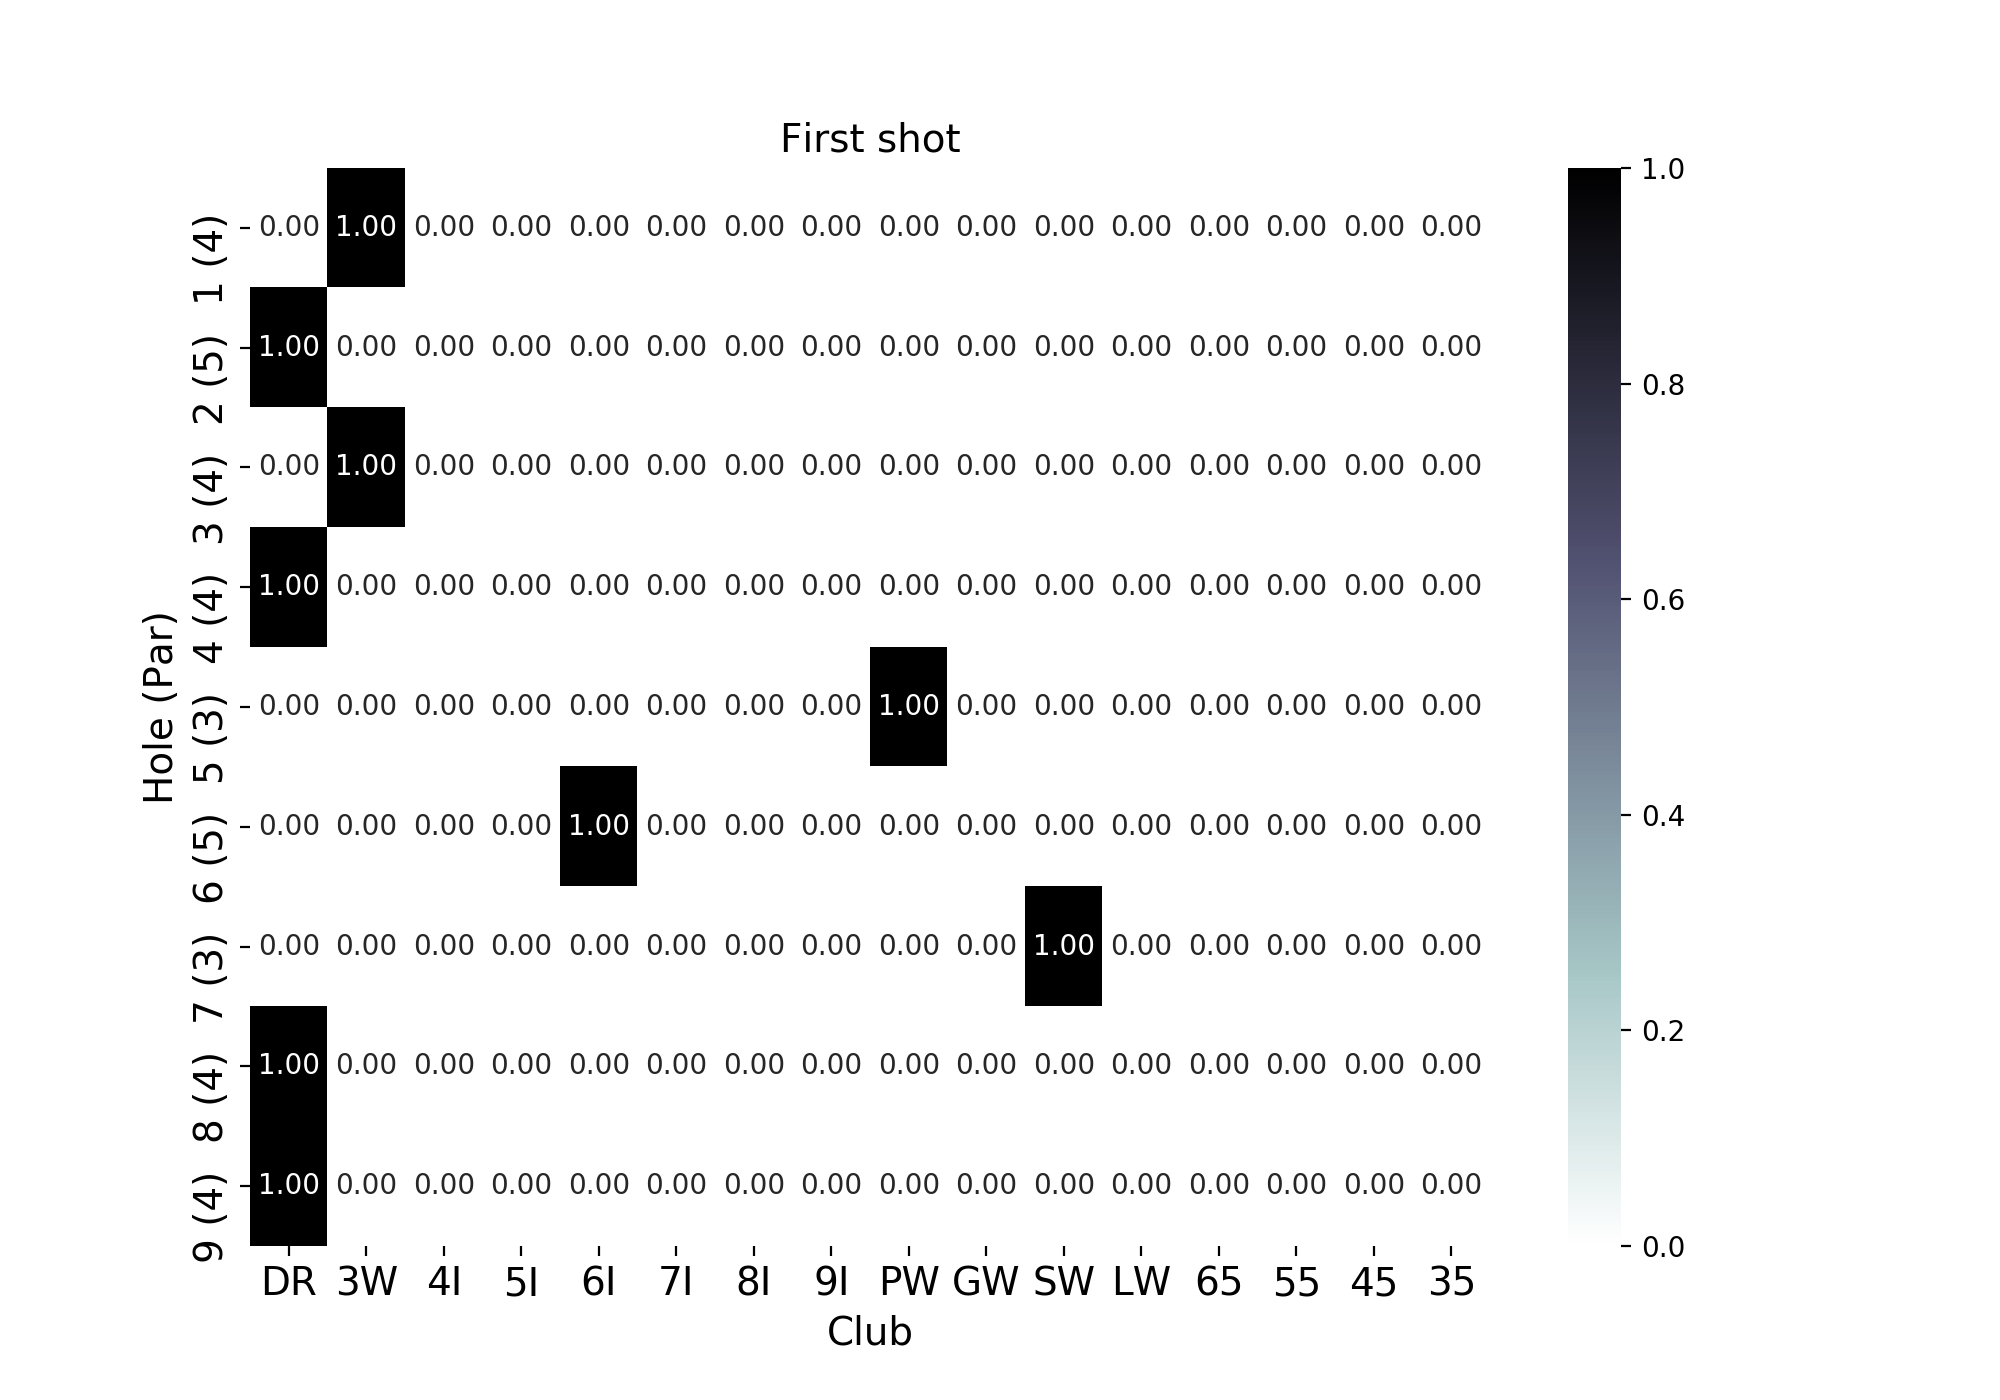
\includegraphics[height=0.3\textheight]{AgentClubChoices/DDDQN_Pebble_Club_Choices_First_Shot.png} 
    \end{subfigure}
    \begin{subfigure}{\textwidth}
    \centering
    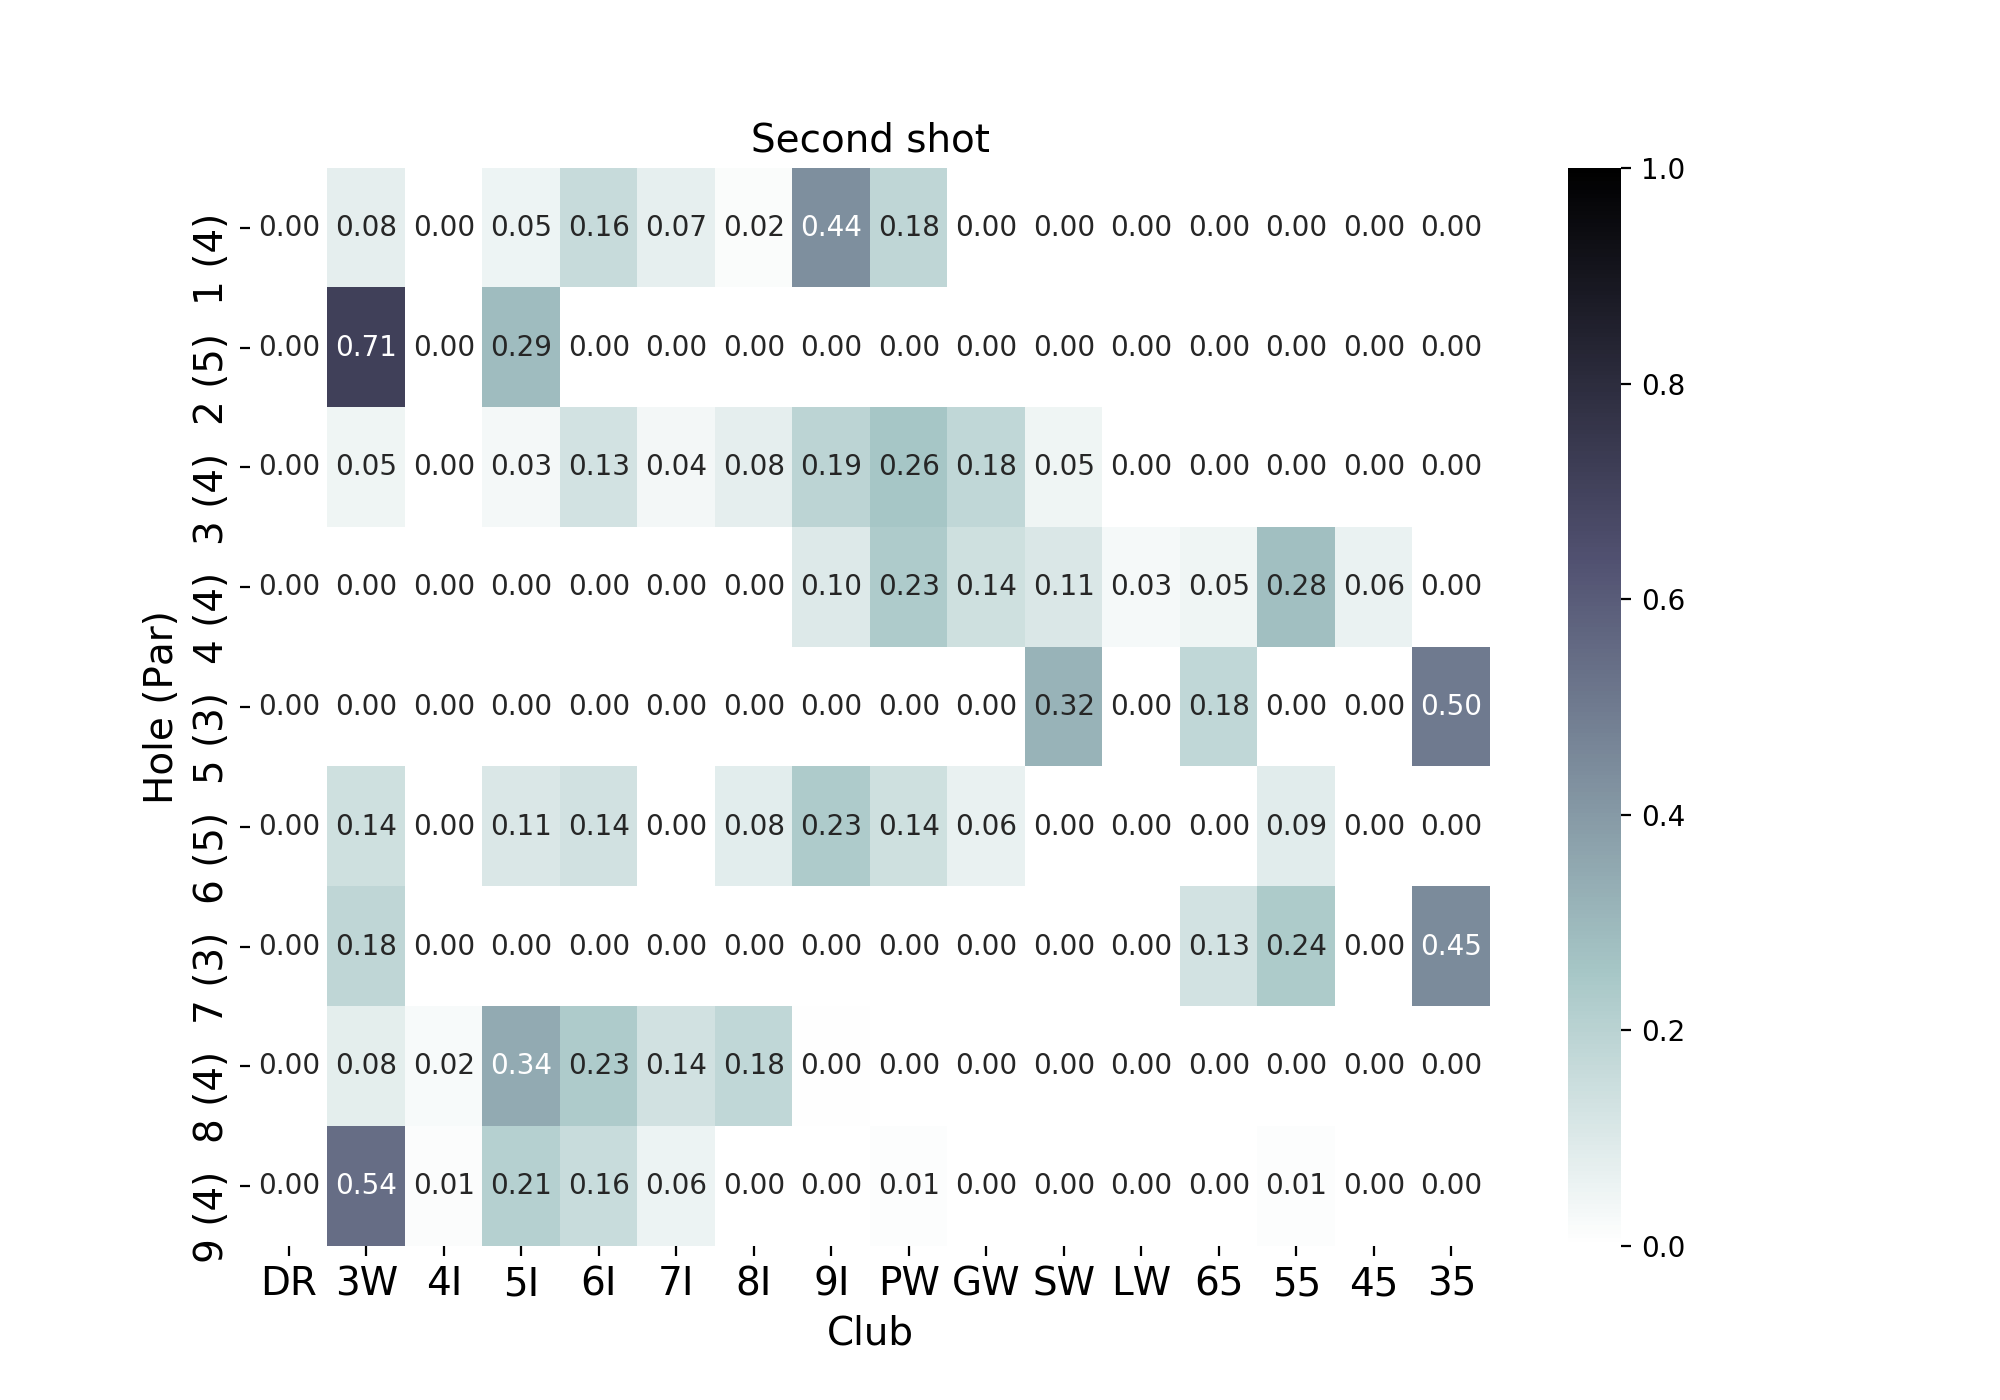
\includegraphics[height=0.3\textheight]{AgentClubChoices/DDDQN_Pebble_Club_Choices_Second_Shot.png} 
    \end{subfigure}
    \begin{subfigure}{\textwidth}
    \centering
    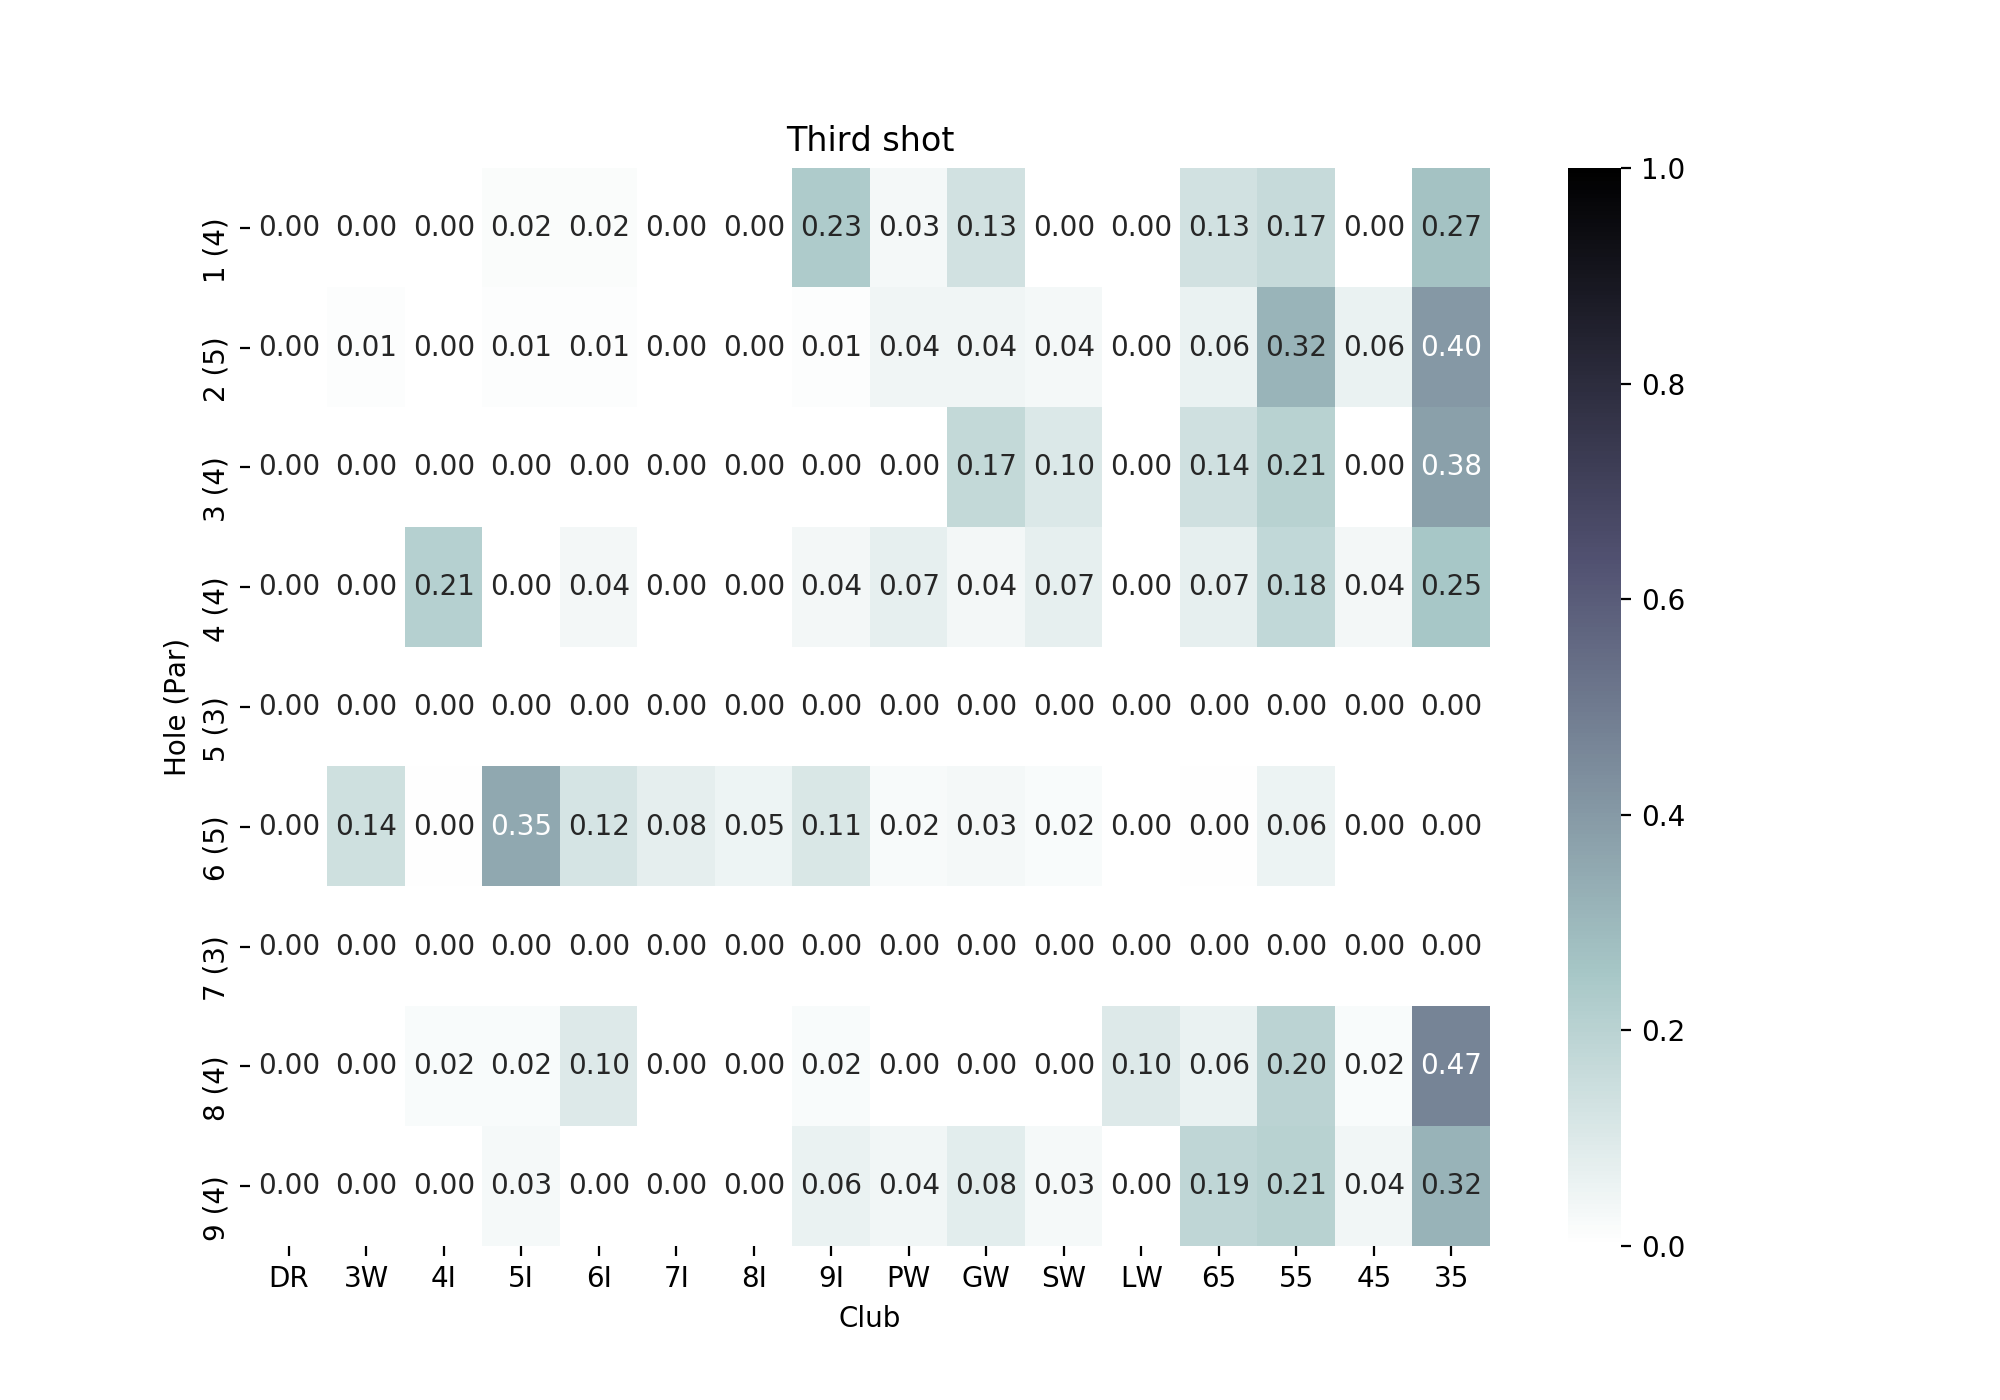
\includegraphics[height=0.3\textheight]{AgentClubChoices/DDDQN_Pebble_Club_Choices_Third_Shot.png} 
    \end{subfigure}
    \caption{Confusion matrices indicating how often clubs were chosen by the Dueling DDQN agent for the first, second and third shot on a given hole at Pebble Beach. Only the first three shots are shown because most of the holes played were completed within this shot range.}
    \label{fig:DDDQN_pebble_club_choice_confusion}
\end{figure}

\begin{figure}
    \centering
    \begin{subfigure}{\textwidth}
    \centering
    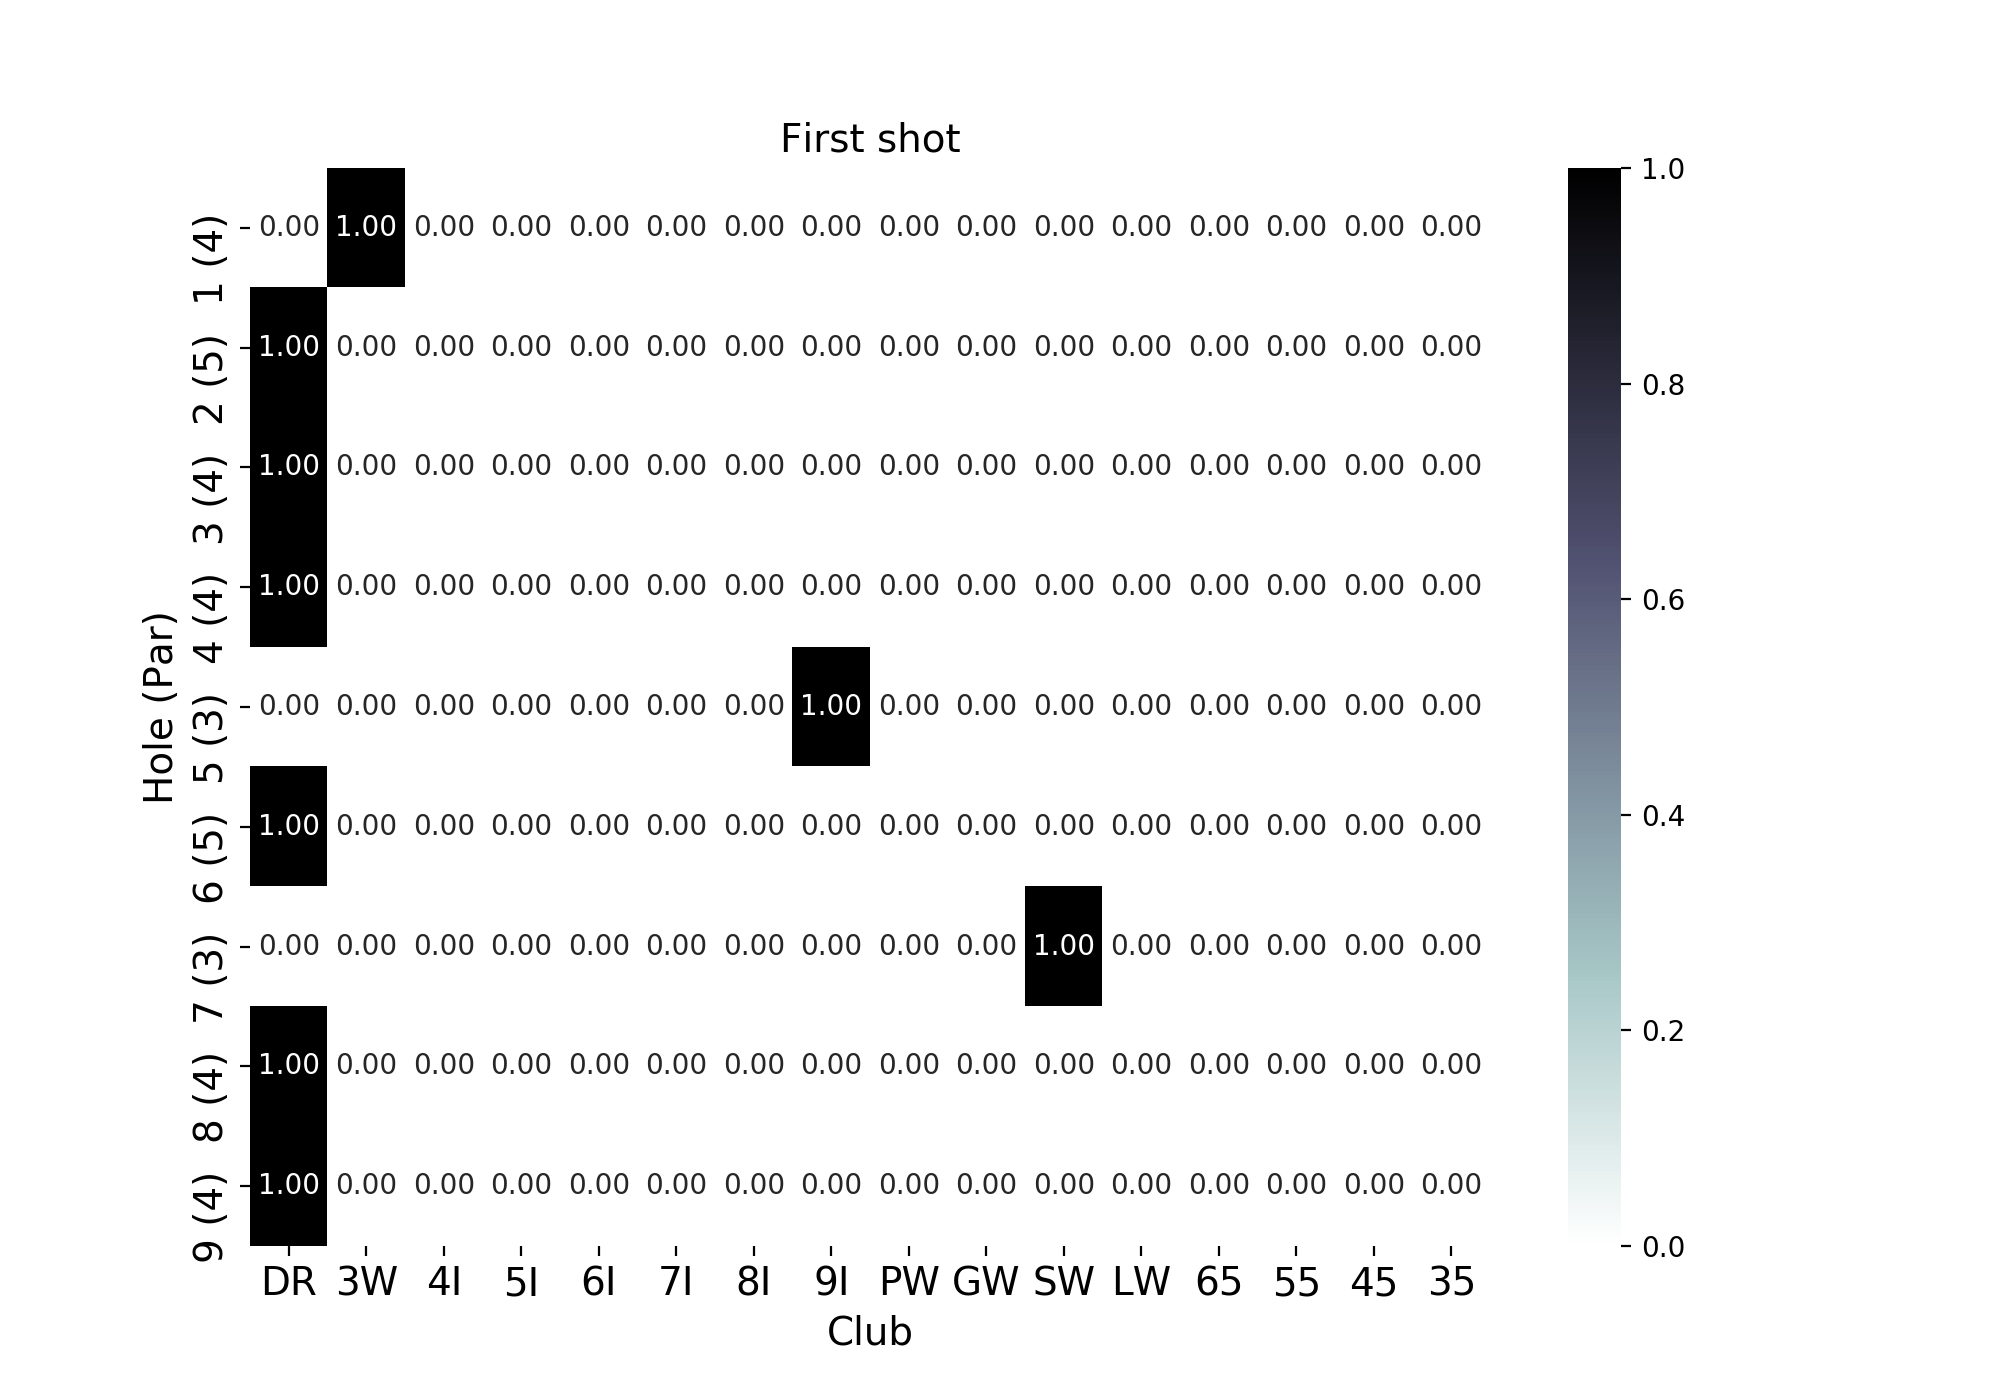
\includegraphics[height=0.3\textheight]{AgentClubChoices/MPDQN_Pebble_Club_Choices_First_Shot.png} 
    \end{subfigure}
    \begin{subfigure}{\textwidth}
    \centering
    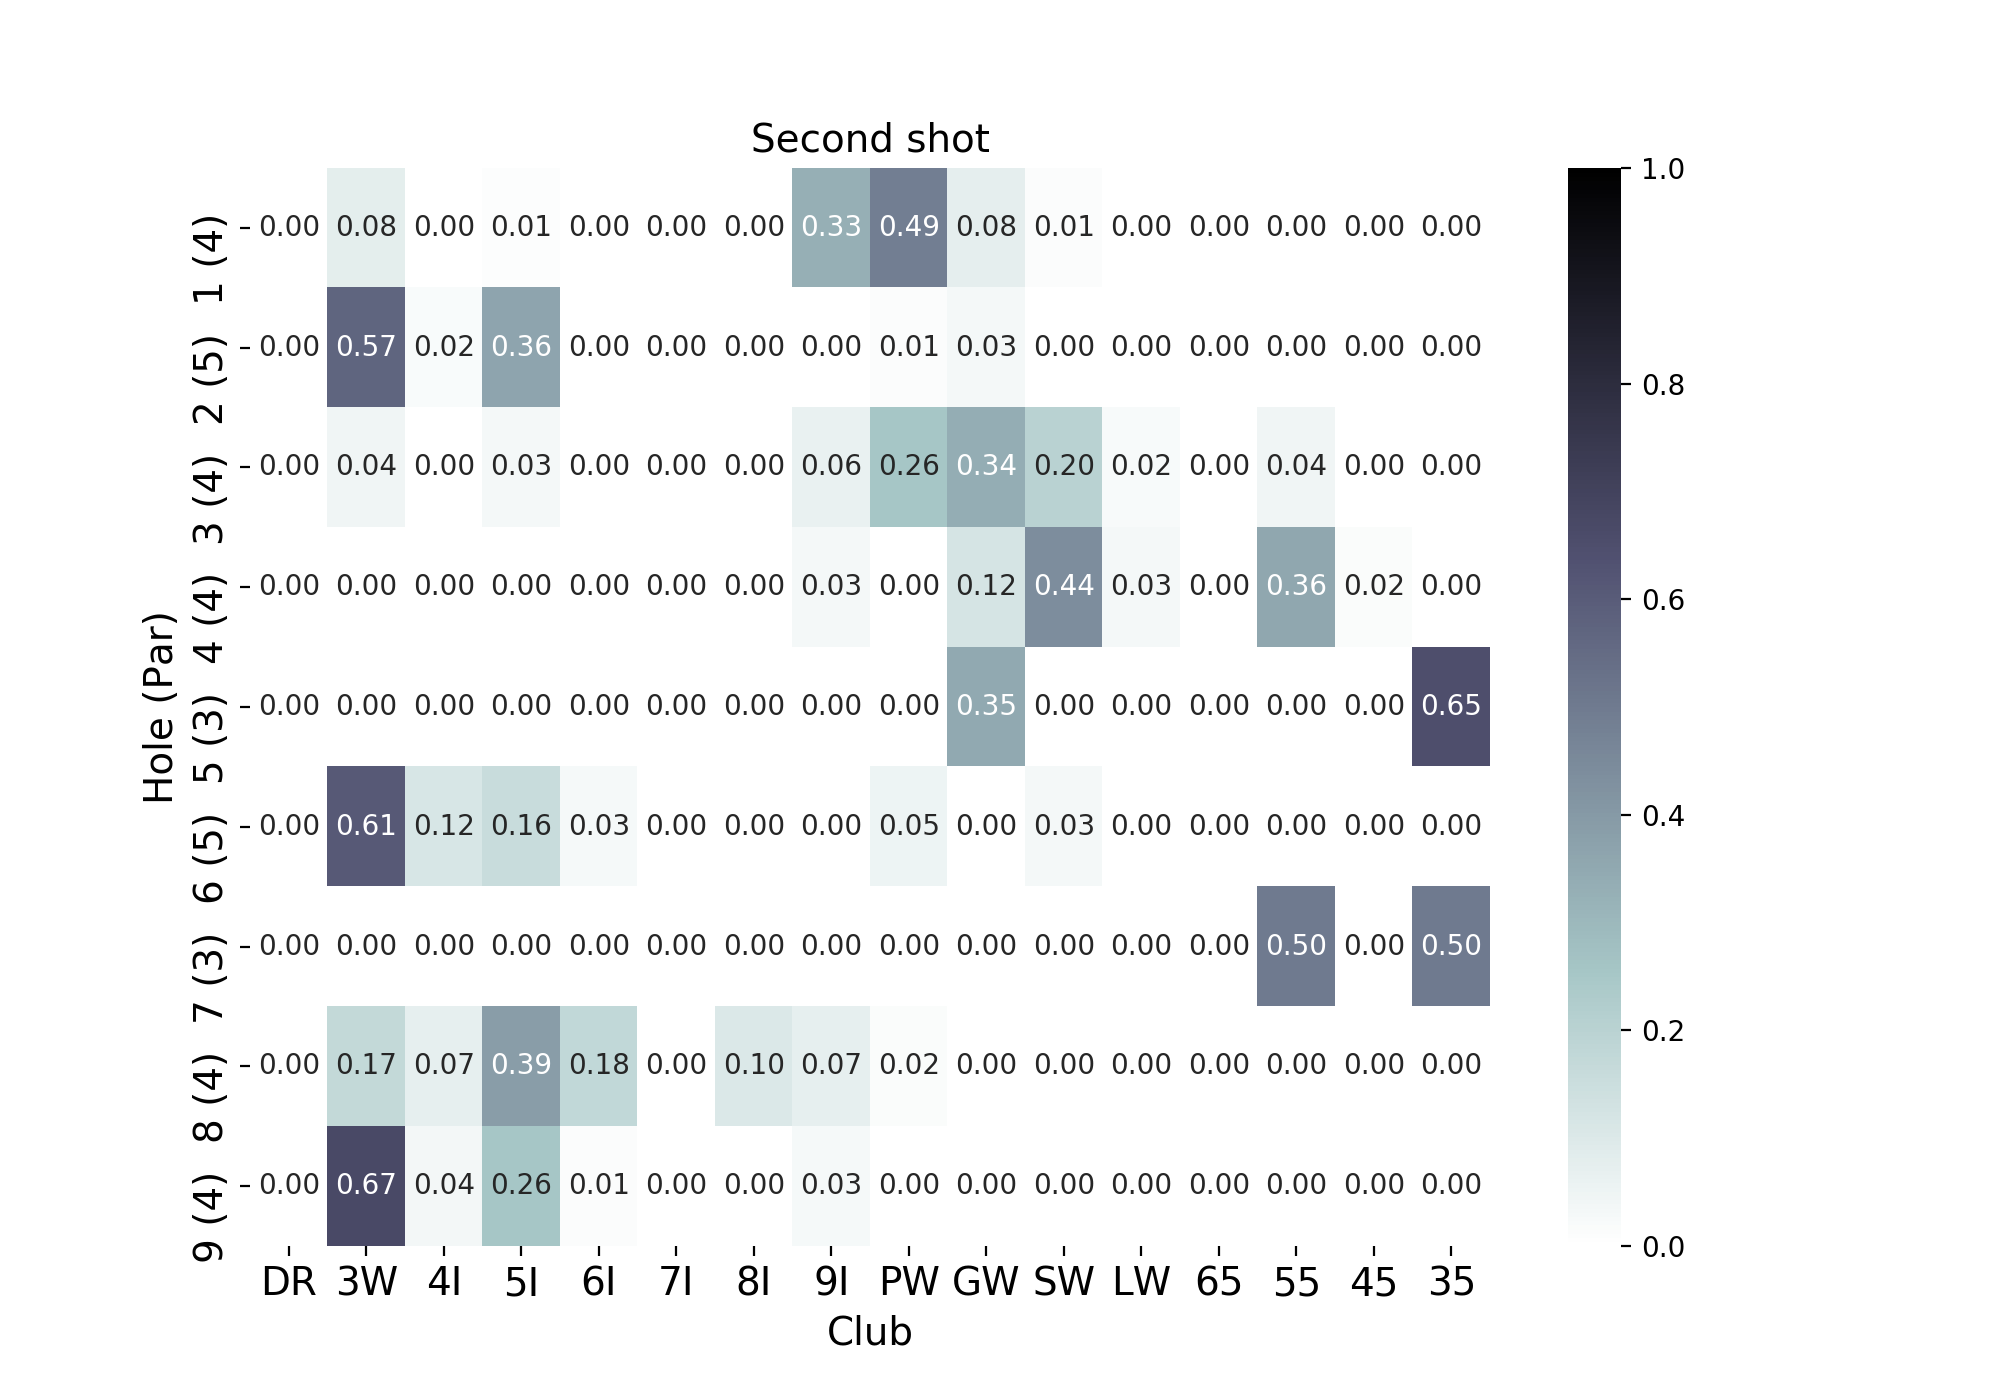
\includegraphics[height=0.3\textheight]{AgentClubChoices/MPDQN_Pebble_Club_Choices_Second_Shot.png} 
    \end{subfigure}
    \begin{subfigure}{\textwidth}
    \centering
    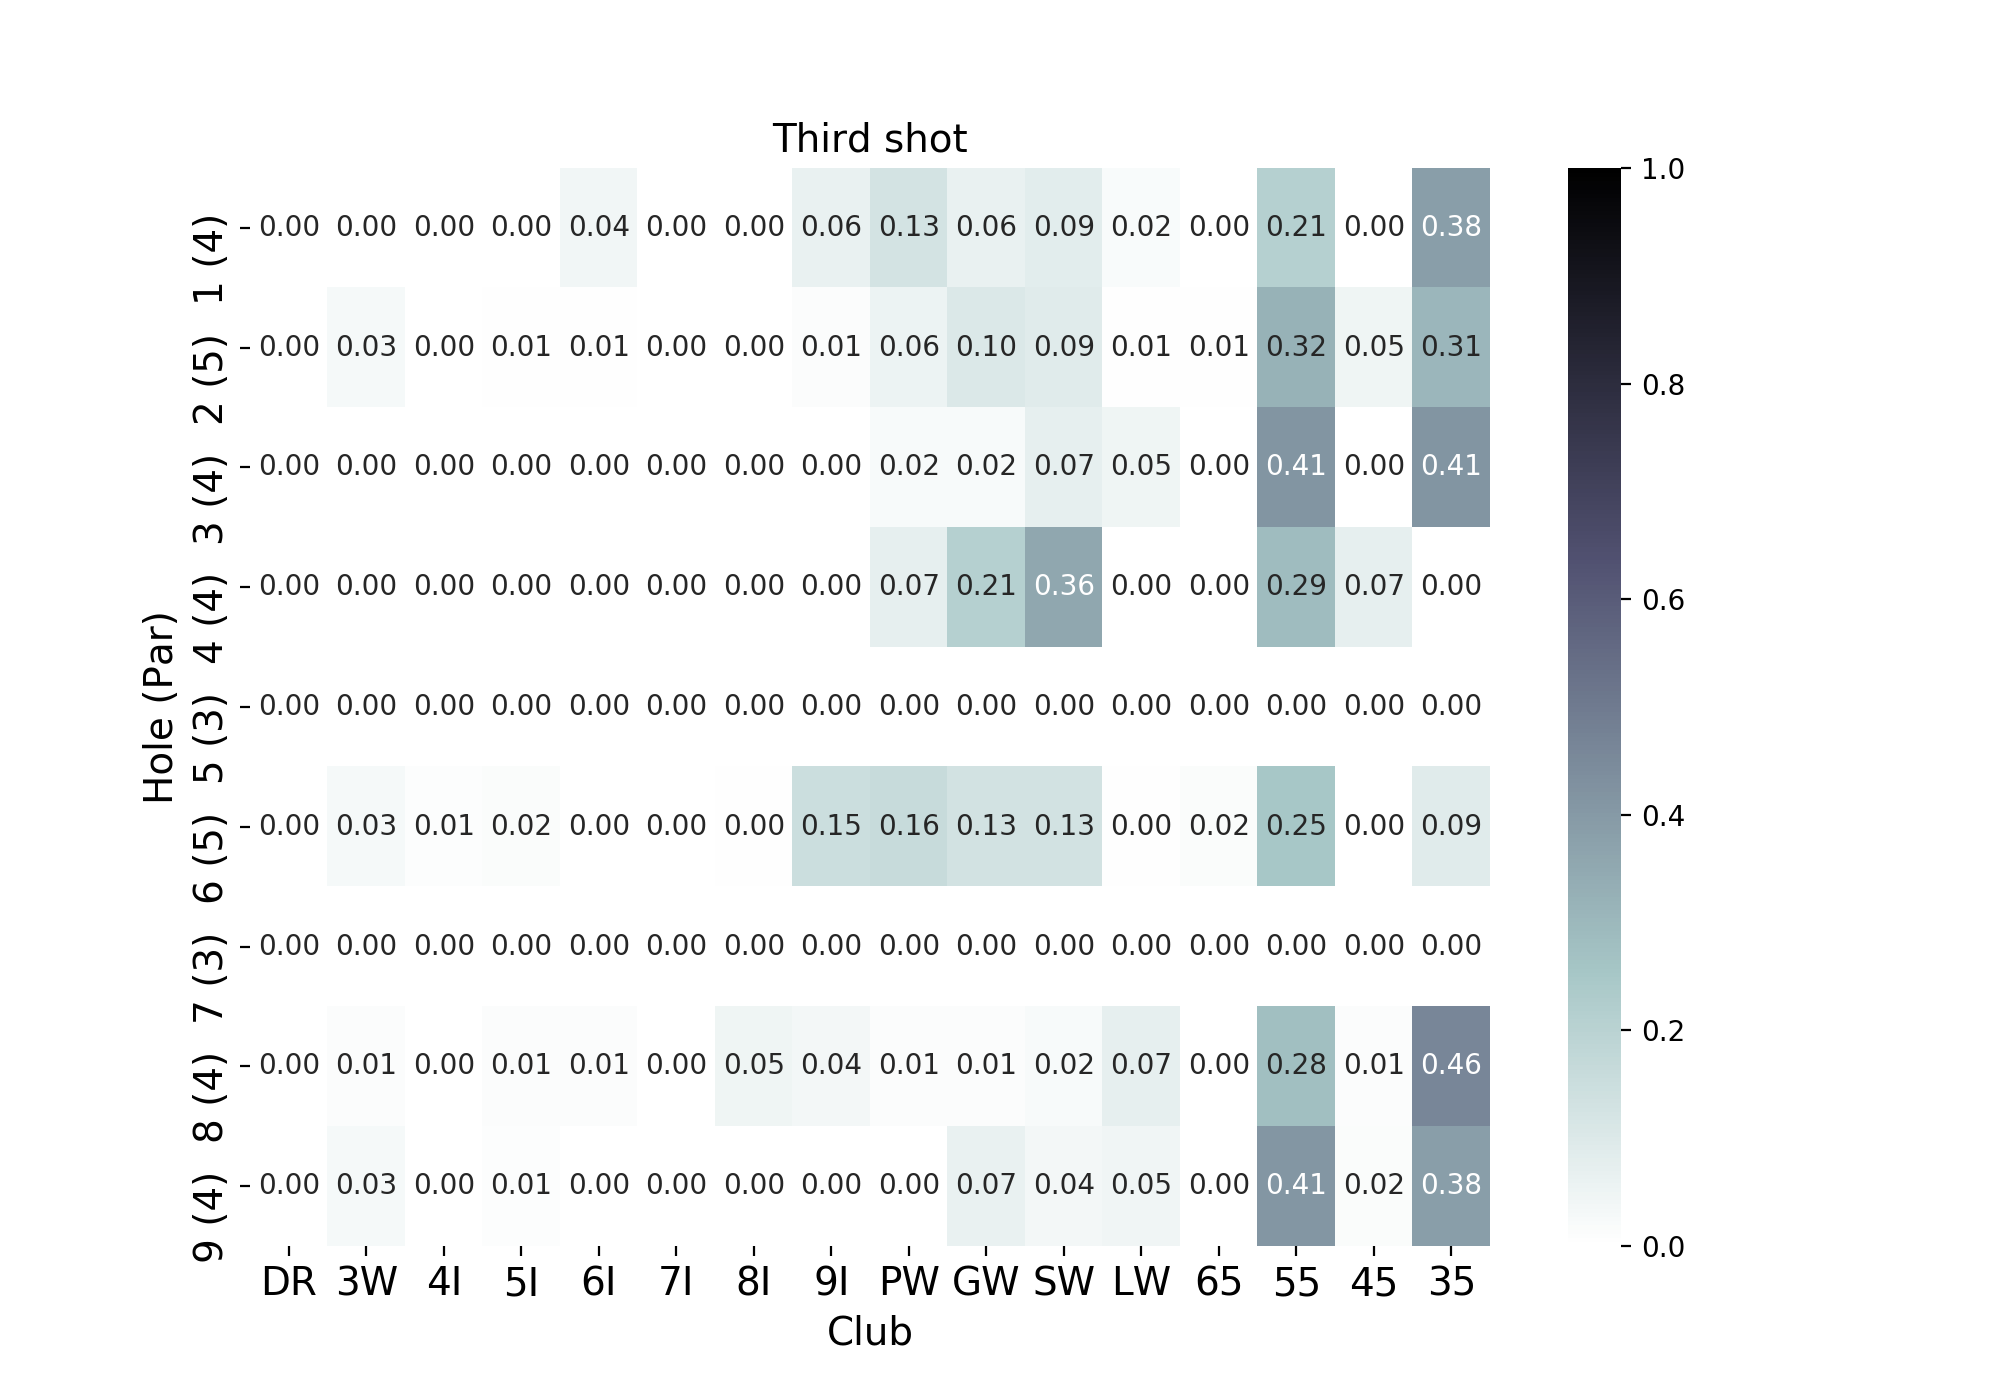
\includegraphics[height=0.3\textheight]{AgentClubChoices/MPDQN_Pebble_Club_Choices_Third_Shot.png} 
    \end{subfigure}
    \caption{Confusion matrices indicating how often clubs were chosen by the MP-DQN agent for the first, second and third shot on a given hole at Pebble Beach. Only the first three shots are shown because most of the holes played were completed within this shot range.}
    \label{fig:MPDQN_pebble_club_choice_confusion}
\end{figure}

\chapter{Ullna GC Histograms}
\label{app:ullna_histograms}
\begin{figure}
    \centering
    \begin{subfigure}{\textwidth}
    \centering
    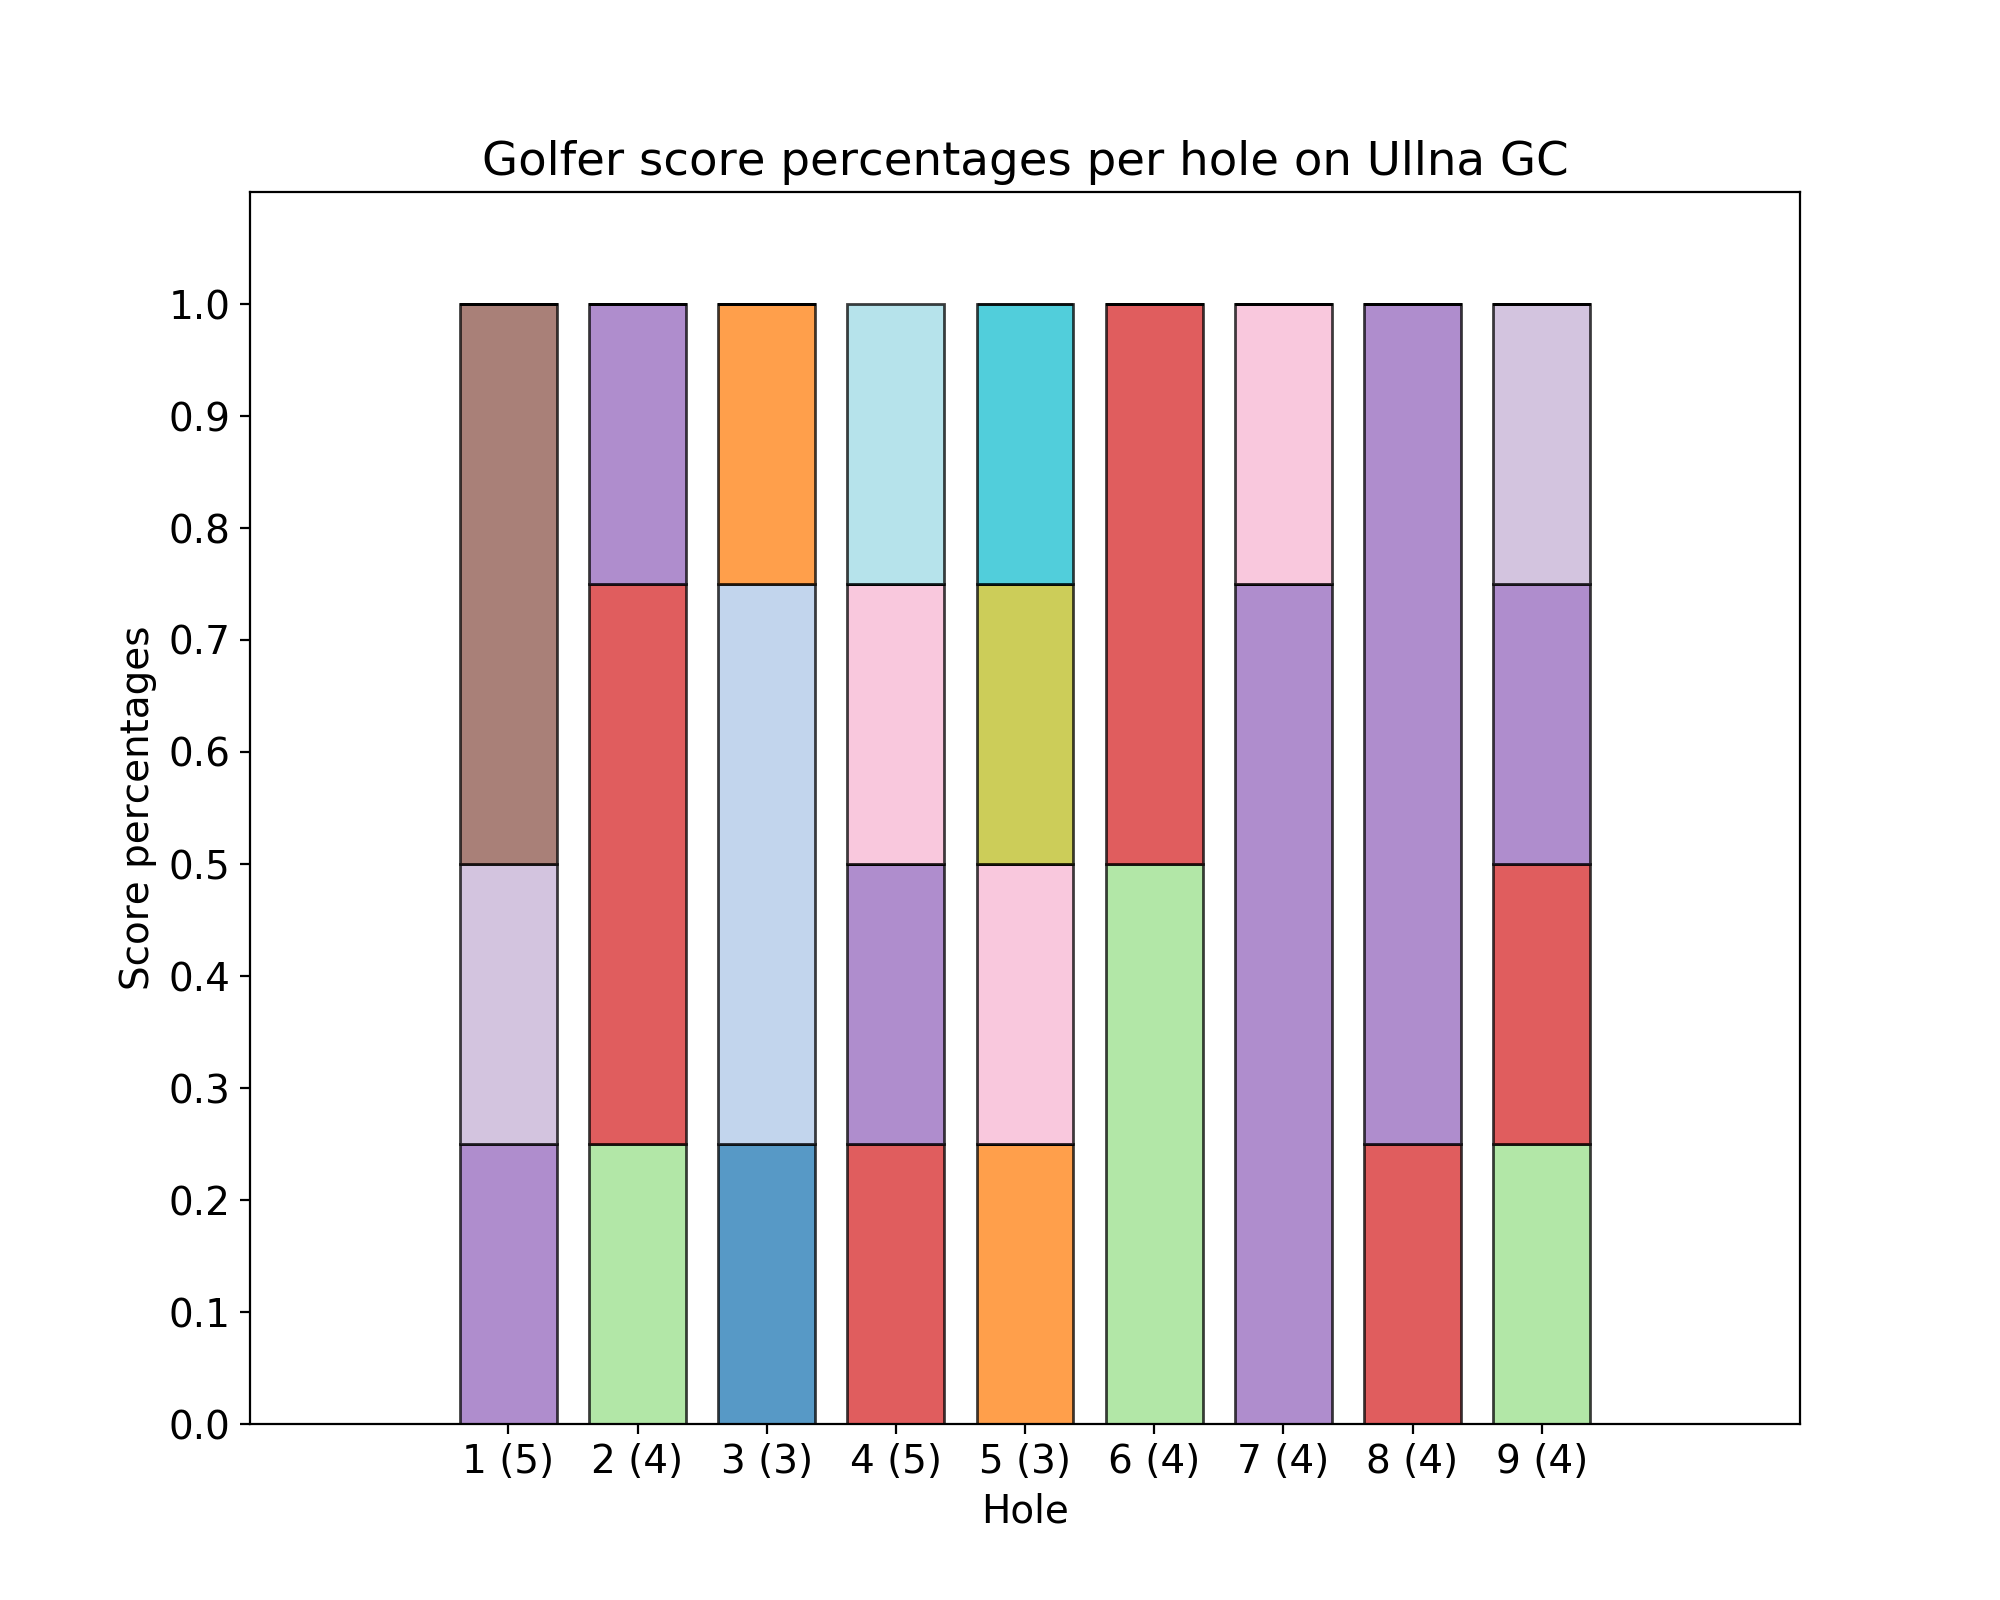
\includegraphics[height=0.3\textheight]{L2Percentages/L2_Score_Percentages_Ullna.png} 
    \end{subfigure}
    \begin{subfigure}{\textwidth}
    \centering
    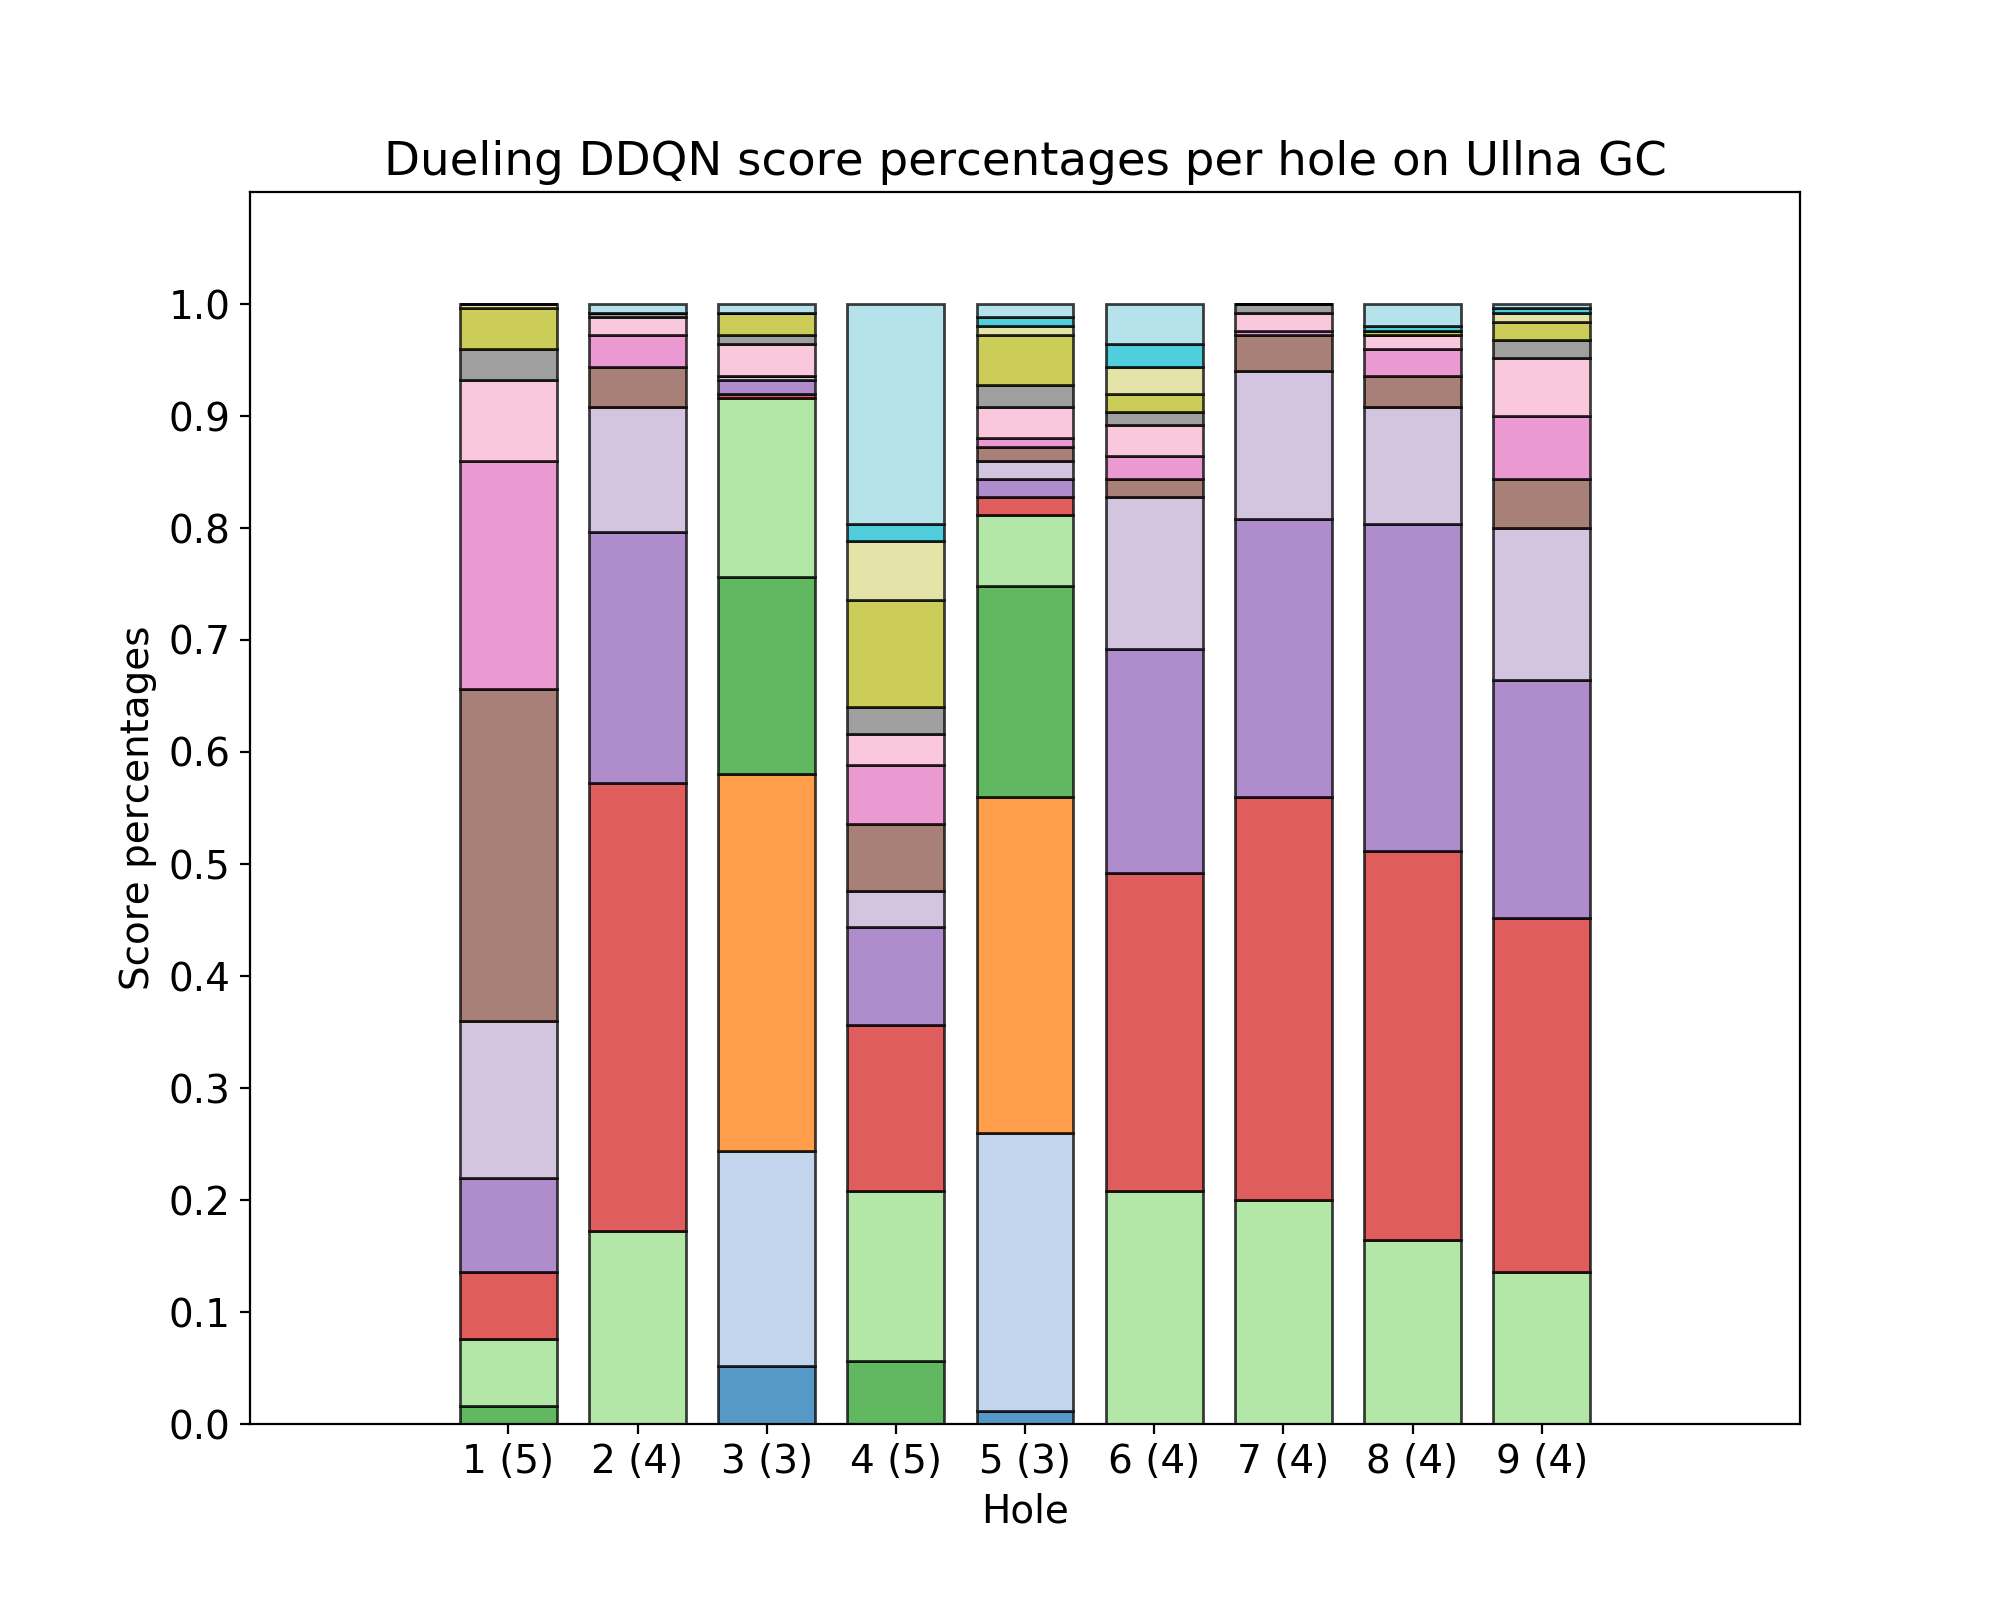
\includegraphics[height=0.3\textheight]{AgentPercentages/DDDQN_Score_Percentages_Ullna.png} 
    \end{subfigure}
    \begin{subfigure}{\textwidth}
    \centering
    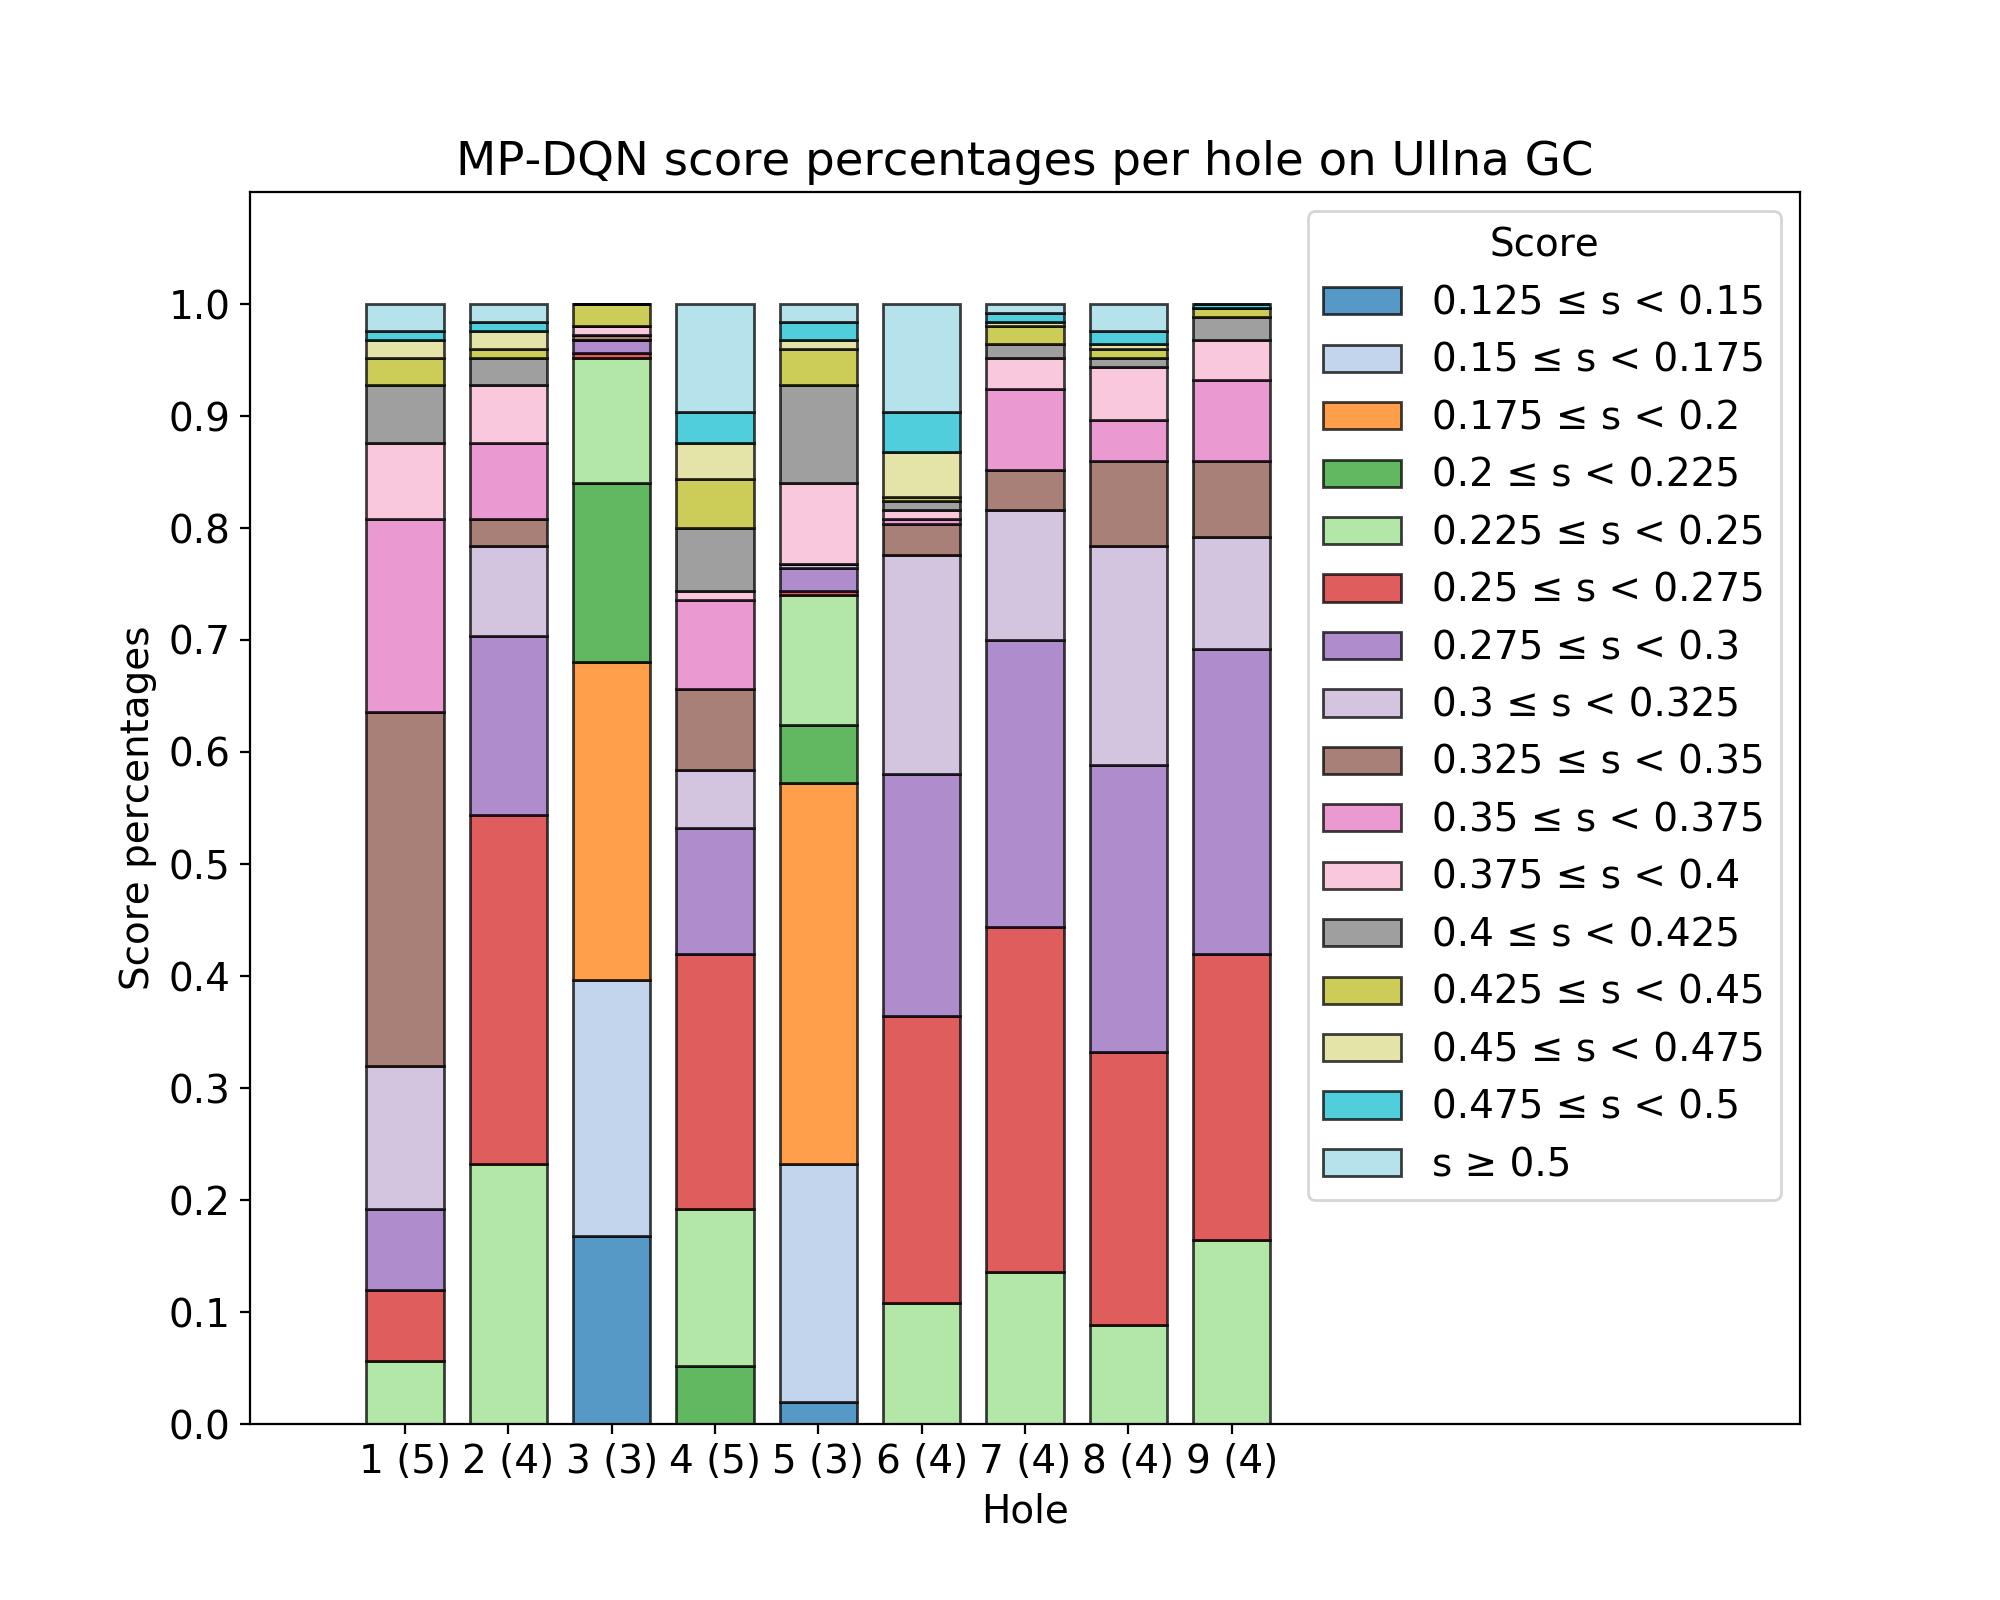
\includegraphics[height=0.3\textheight]{AgentPercentages/MPDQN_Score_Percentages_Ullna.png} 
    \end{subfigure}
    \caption{Histograms showcasing how often different scores were achieved on Ullna GC by the golfer, Dueling DDQN agent and MP-DQN agent, respectively.}
    \label{fig:ullna_score_histograms}
\end{figure}

\begin{figure}
    \centering
    \begin{subfigure}{\textwidth}
    \centering
    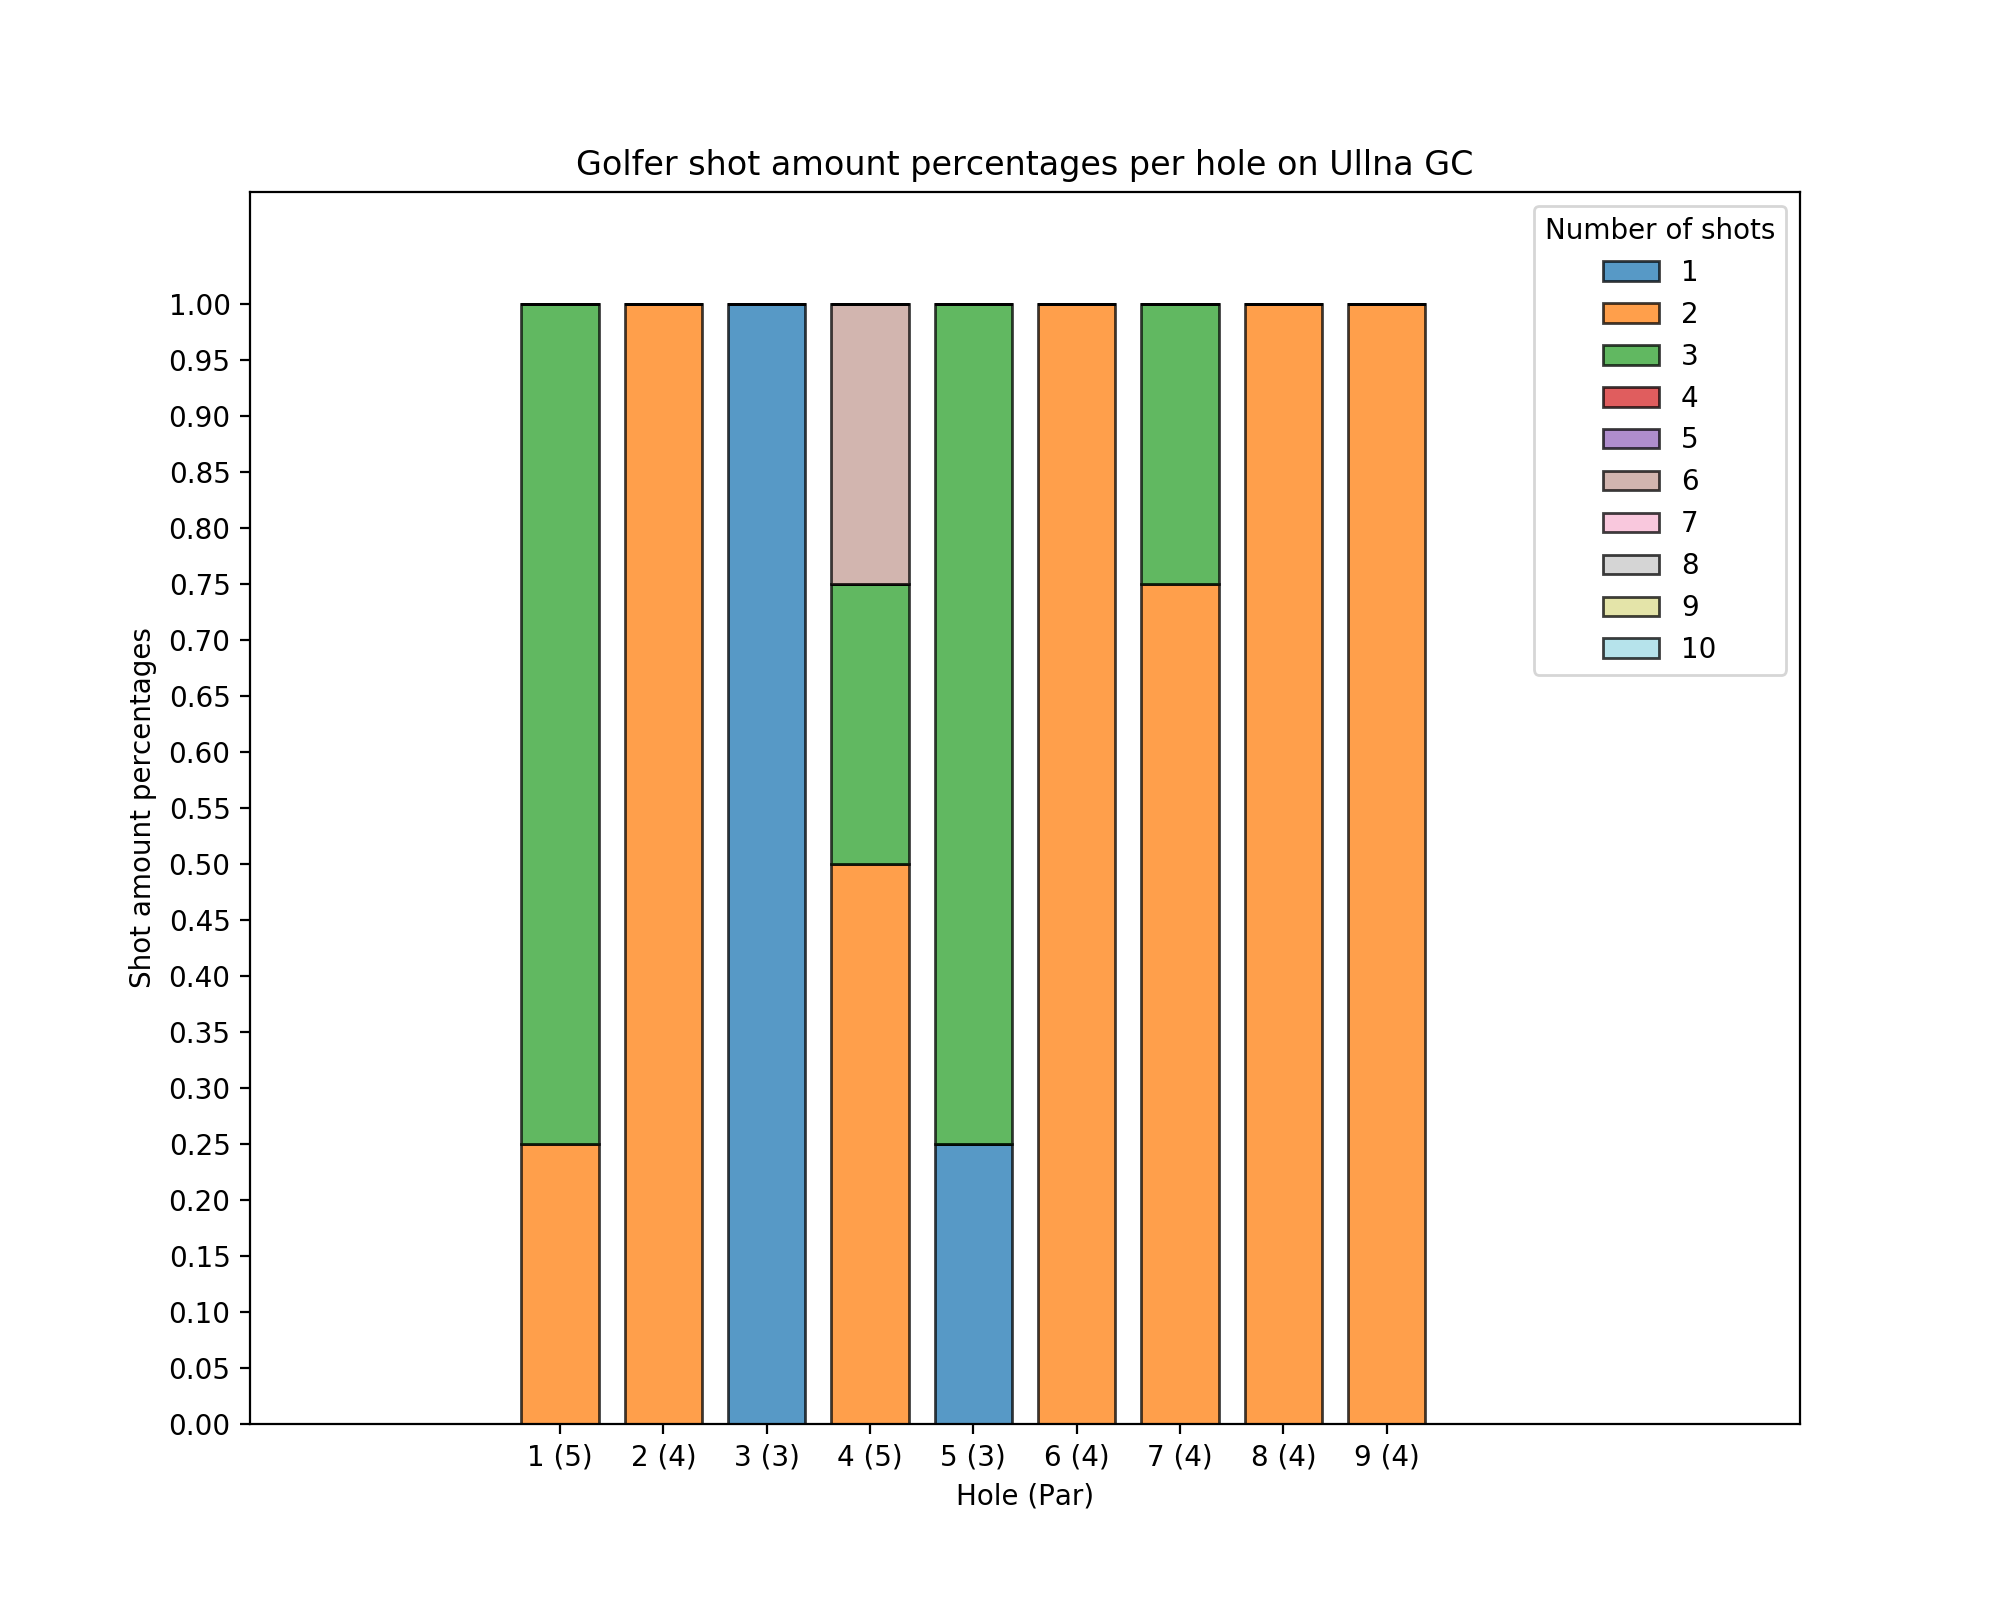
\includegraphics[height=0.3\textheight]{L2Percentages/L2_Shot_Percentages_Ullna.png} 
    \end{subfigure}
    \begin{subfigure}{\textwidth}
    \centering
    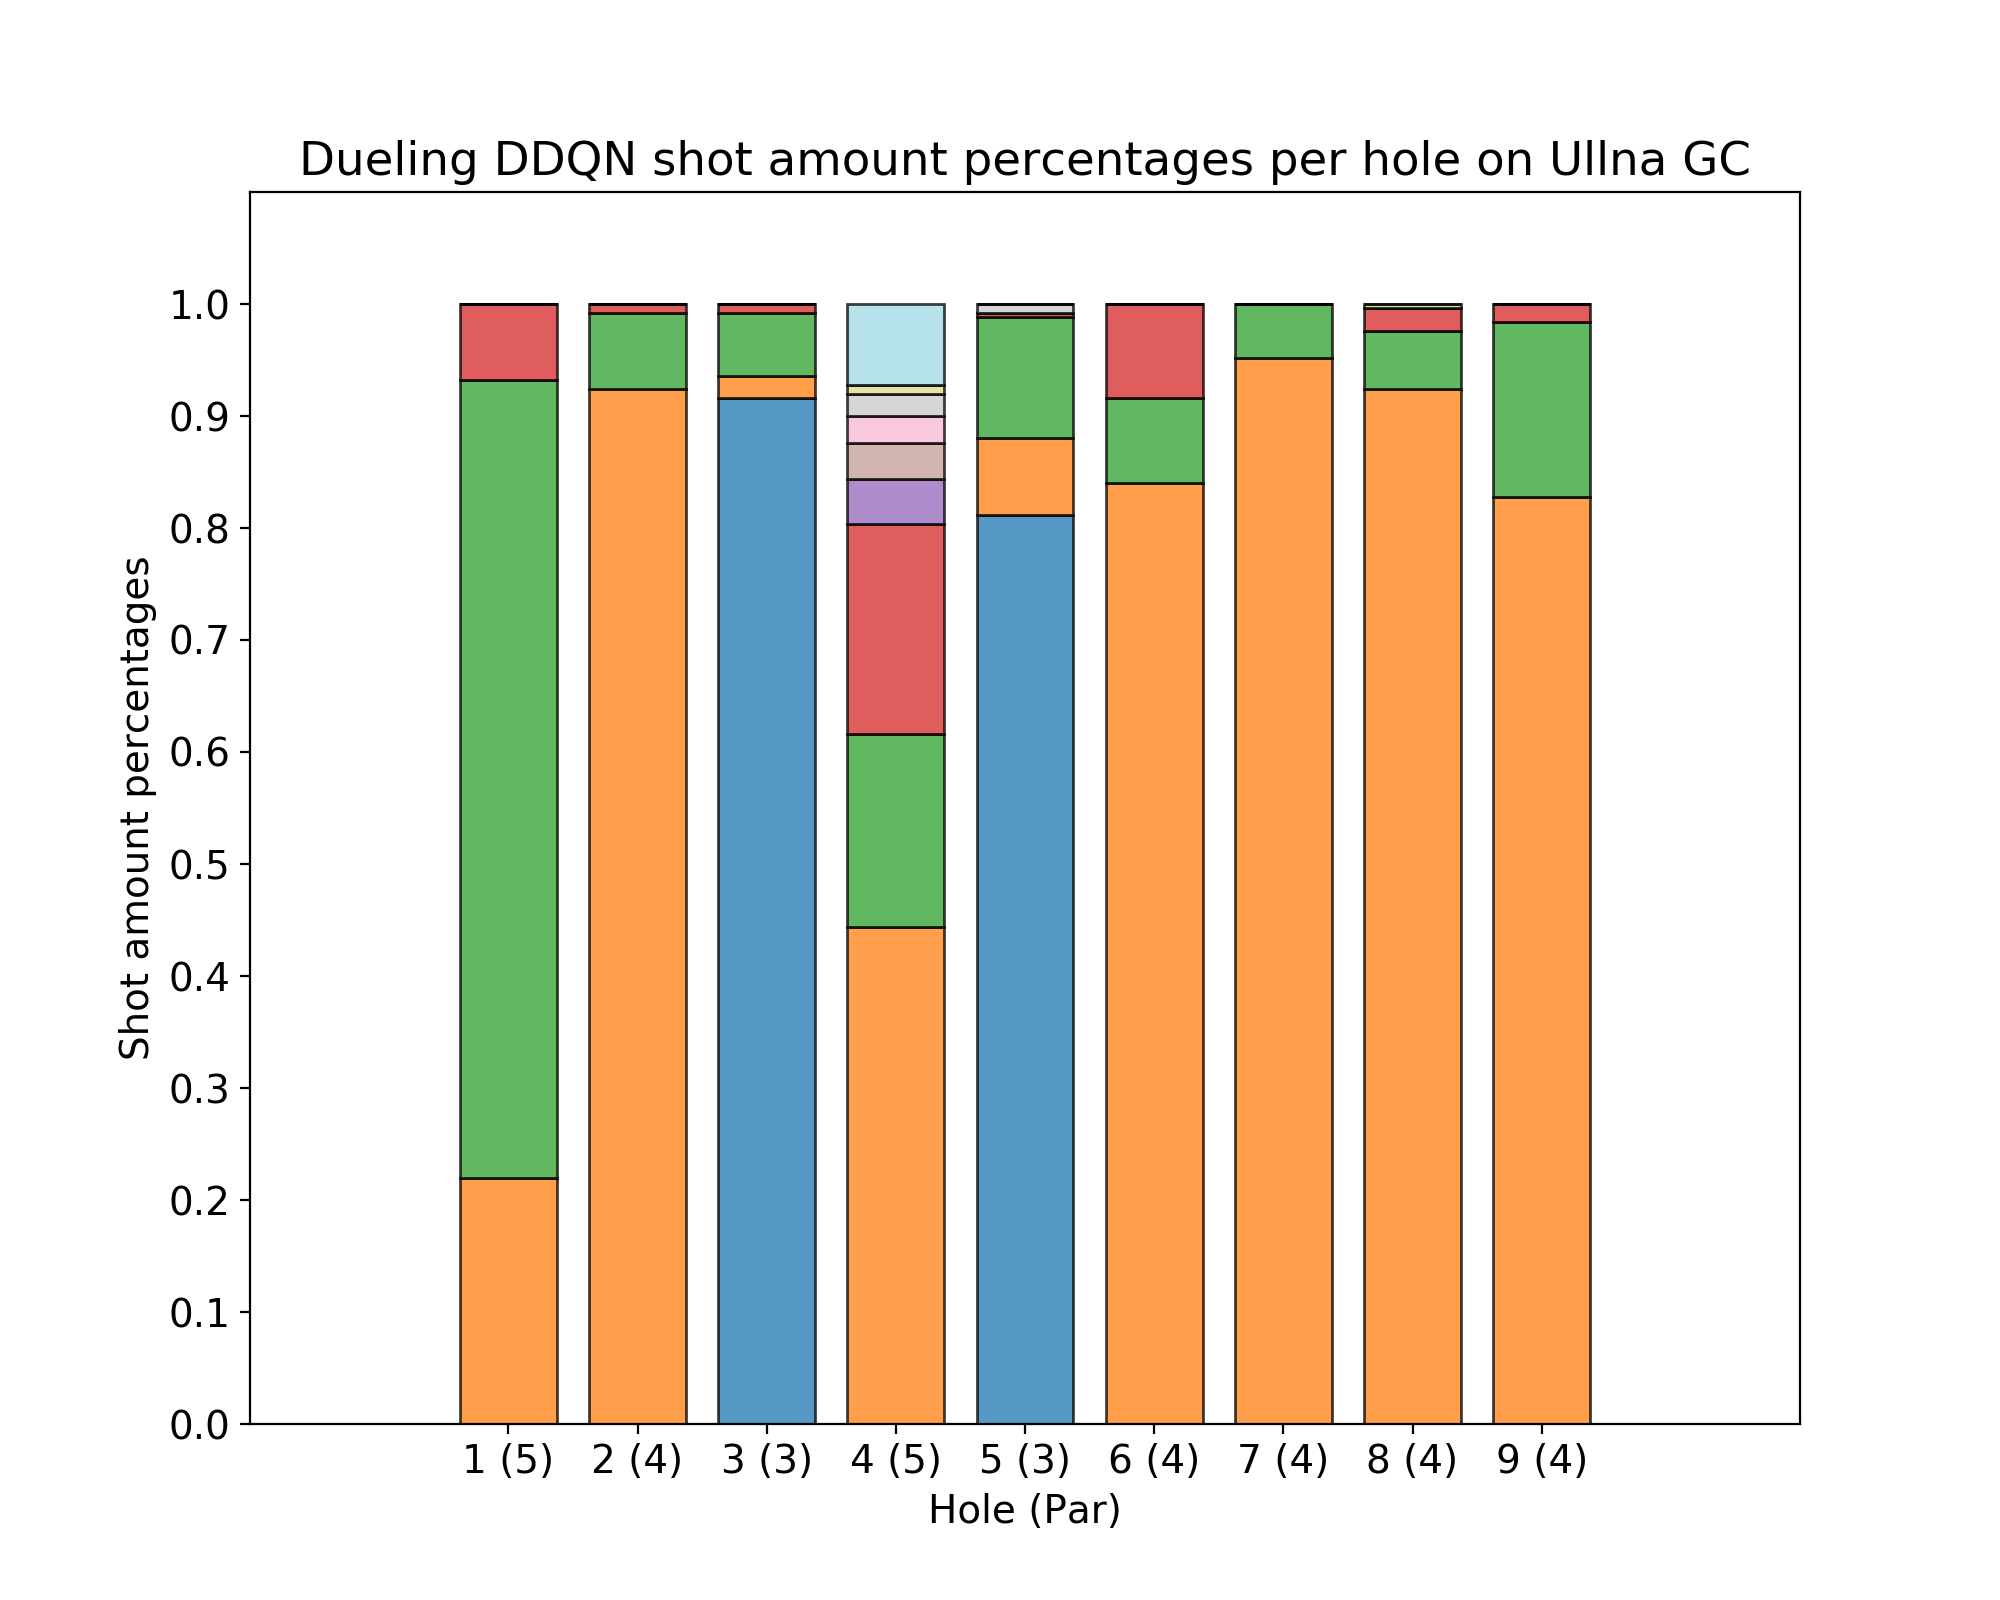
\includegraphics[height=0.3\textheight]{AgentPercentages/DDDQN_Shot_Percentages_Ullna.png} 
    \end{subfigure}
    \begin{subfigure}{\textwidth}
    \centering
    \includegraphics[height=0.3\textheight]{AgentPercentages/MPDQN_Shot_Percentages_Ullna.png} 
    \end{subfigure}
    \caption{Histograms showcasing how often different shot amounts were achieved on Ullna GC by the golfer, Dueling DDQN agent and MP-DQN agent, respectively.}
    \label{fig:ullna_shot_histograms}
\end{figure}

\begin{figure}
    \centering
    \begin{subfigure}{\textwidth}
    \centering
    \includegraphics[height=0.3\textheight]{L2Percentages/L2_Distance_Percentages_Ullna.png} 
    \end{subfigure}
    \begin{subfigure}{\textwidth}
    \centering
    \includegraphics[height=0.3\textheight]{AgentPercentages/DDDQN_Distance_Percentages_Ullna.png} 
    \end{subfigure}
    \begin{subfigure}{\textwidth}
    \centering
    \includegraphics[height=0.3\textheight]{AgentPercentages/MPDQN_Distance_Percentages_Ullna.png} 
    \end{subfigure}
    \caption{Histograms showcasing how often different distances remaining were achieved on Ullna GC by the golfer, Dueling DDQN agent and MP-DQN agent, respectively.}
    \label{fig:ullna_distance_histograms}
\end{figure}

\chapter{Ullna GC Club Choices}
\label{app:ullna_club_choices}
\begin{figure}
    \centering
    \begin{subfigure}{\textwidth}
    \centering
    \includegraphics[height=0.3\textheight]{L2ClubChoices/Ludvig_Ullna_Club_Choices_First_Shot.png} 
    \end{subfigure}
    \begin{subfigure}{\textwidth}
    \centering
    \includegraphics[height=0.3\textheight]{L2ClubChoices/Ludvig_Ullna_Club_Choices_Second_Shot.png} 
    \end{subfigure}
    \begin{subfigure}{\textwidth}
    \centering
    \includegraphics[height=0.3\textheight]{L2ClubChoices/Ludvig_Ullna_Club_Choices_Third_Shot.png} 
    \end{subfigure}
    \caption{Confusion matrices indicating how often clubs were chosen by the golfer for the first, second and third shot on a given hole at Ullna GC. Only the first three shots are shown because most of the holes played were completed within this shot range.}
    \label{fig:L2_ullna_club_choice_confusion}
\end{figure}

\begin{figure}
    \centering
    \begin{subfigure}{\textwidth}
    \centering
    \includegraphics[height=0.3\textheight]{AgentClubChoices/DDDQN_Ullna_Club_Choices_First_Shot.png} 
    \end{subfigure}
    \begin{subfigure}{\textwidth}
    \centering
    \includegraphics[height=0.3\textheight]{AgentClubChoices/DDDQN_Ullna_Club_Choices_Second_Shot.png} 
    \end{subfigure}
    \begin{subfigure}{\textwidth}
    \centering
    \includegraphics[height=0.3\textheight]{AgentClubChoices/DDDQN_Ullna_Club_Choices_Third_Shot.png} 
    \end{subfigure}
    \caption{Confusion matrices indicating how often clubs were chosen by the Dueling DDQN agent for the first, second and third shot on a given hole at Ullna GC. Only the first three shots are shown because most of the holes played were completed within this shot range.}
    \label{fig:DDDQN_ullna_club_choice_confusion}
\end{figure}

\begin{figure}
    \centering
    \begin{subfigure}{\textwidth}
    \centering
    \includegraphics[height=0.3\textheight]{AgentClubChoices/MPDQN_Ullna_Club_Choices_First_Shot.png} 
    \end{subfigure}
    \begin{subfigure}{\textwidth}
    \centering
    \includegraphics[height=0.3\textheight]{AgentClubChoices/MPDQN_Ullna_Club_Choices_Second_Shot.png} 
    \end{subfigure}
    \begin{subfigure}{\textwidth}
    \centering
    \includegraphics[height=0.3\textheight]{AgentClubChoices/MPDQN_Ullna_Club_Choices_Third_Shot.png} 
    \end{subfigure}
    \caption{Confusion matrices indicating how often clubs were chosen by the MP-DQN agent for the first, second and third shot on a given hole at Ullna GC. Only the first three shots are shown because most of the holes played were completed within this shot range.}
    \label{fig:MPDQN_ullna_club_choice_confusion}
\end{figure}

\chapter{Miscellaneous}
\begin{table}
    \centering
    \begin{tabular}{c|c}
        \textbf{Area} & \textbf{Integer} \\ \hline
        Fairway & 0 \\ 
        Rough & 1 \\ 
        Green & 2 \\ 
        Tee box & 3 \\ 
        Pathway & 4 \\ 
        Tree & 5 \\ 
        Out of bounds & 6 \\ 
        Water & 7 \\ 
        Ball & 8 \\ 
        Hole & 9 \\ 
        Bunker & 10 \\ 
        Waste area & 11 \\ 
        Native area & 12 \\ 
        Penalty area & 13 \\ 
    \end{tabular}
    \caption{A table indicating the mapping between golf areas and integers. These integers were stored in the observations from the golf simulation application and used by the agent to learn how to play golf.}
    \label{app:tab:areamapping}
\end{table}

\tailmatter

\end{document}
